%!TEX TS-program = xelatex

%!TEX root = ../Thesis.tex

% This information is used in titlepage, colophon, preface and hyperref setup (pdf metainfo), and other options.

%\def\thesistypeabbr{B.Eng.}
%\def\thesistype    {Bachelor of Engineering}
%\def\thesistypeabbr{B.Sc.Eng.}
%\def\thesistype    {Bachelor of Science in Engineering}
%\def\thesistypeabbr{M.Sc.}
%\def\thesistype    {Master of Science in Engineering}
\def\thesistypeabbr{Ph.D.}
\def\thesistype    {Doctor of Philosophy}

\def\thesisauthor  {Daniel Esteban Morales Bondy}
%\def\thesistitle   {Validation of Service-providing Aggregators in the Future Power System}
%\def\thesissubtitle{Service Modeling and Evaluation of Aggregator Architectures} %\protect\\
\def\thesistitle   {Demand Response for a Secure Power System Operation}
\def\thesissubtitle{Service Specification, Validation and Verification in View of Distributed Energy Systems} %\protect\\
%\def\thesistitle   {Service Modeling and Evaluation of Service-providing Aggregators in the Future Power System}
%\def\thesissubtitle{Towards Aggregator Validation}
\def\thesislocation{Ris{\o}}

%\def\papersize    {b5paper} % Final papersize (b5paper/a4paper), recommended papersize for DTU Compute is b5paper
\def\showtrims    {false} % Print on larger paper than \papersize and show trim marks (true/false)?

\def\showtodos    {true}  % Show todos (true/false)?
\def\confidential {false} % Confidential thesis (true/false)?


%!TEX root = ../Thesis.tex
\RequirePackage[l2tabu,orthodox]{nag} % Old habits die hard

\documentclass[a4paper,twoside,justified]{tufte-book}
\RequireXeTeX


% Large environments
%\usepackage{microtype}
\usepackage{mathtools}
\usepackage{listings}                 % Source code printer for LaTeX
\usepackage{tikz}
\usepackage{fontspec}
\defaultfontfeatures{Ligatures=TeX}
%\setmainfont{Junicode}

\usepackage{makeidx}



% Links
%\usepackage[hyphens]{url}             % Allow hyphens in URL's
%\makeatletter
%%% Adjust so gatherings is allowd for single sheets too! (hacking functions in memoir.dtx)
%%\patchcmd{\leavespergathering}{\ifnum\@memcnta<\tw@}{\ifnum\@memcnta<\@ne}{
%%    \leavespergathering{1}
%%    % Insert the frieze
%%    \patchcmd{\@memensuresigpages}{\repeat}{\repeat\frieze}{}{}
%%}{}
%%\makeatother\usepackage[unicode=false,psdextra]{hyperref}                 % References package

% Graphics and colors
\usepackage{graphicx}                 % Including graphics and using colours
\usepackage{xcolor}                   % Defined more color names
\usepackage{eso-pic}                  % Watermark and other bag
\usepackage{preamble/dtucolors}
\graphicspath{{graphics/}}

% Language
\usepackage{polyglossia}    % multilingual typesetting and appropriate hyphenation
\setdefaultlanguage{english}

% Floating objets, captions and references
\usepackage[noabbrev,nameinlink,capitalise]{cleveref} % Clever references. Options: "fig. !1!" --> "!Figure 1!"
%\hangcaption
%\captionnamefont{\bfseries}
%\subcaptionlabelfont{\bfseries}
%\newsubfloat{figure}
%\newsubfloat{table}
%\letcountercounter{figure}{table}     % Consecutive table and figure numbering

% Table of contents (TOC)
\setcounter{tocdepth}{1}              % Depth of table of content
\setcounter{secnumdepth}{2}           % Depth of section numbering

% Todos
\usepackage{totcount}                 % For total counting of counters
\def\todoshowing{}
\ifnum\strcmp{\showtodos}{false}=0
    \def\todoshowing{disable}
\fi
\usepackage[colorinlistoftodos,\todoshowing]{todonotes} % Todonotes package for nice todos
\newtotcounter{todocounter}           % Creates counter in todo
\let\oldtodo\todo
\newcommand*{\newtodo}[2][]{\stepcounter{todocounter}\oldtodo[#1]{\thesection~(\thetodocounter)~#2}}
\let\todo\newtodo
\let\oldmissingfigure\missingfigure
\newcommand*{\newmissingfigure}[2][]{\stepcounter{todocounter}\oldmissingfigure[#1]{\thesection~(\thetodocounter)~#2}}
\let\missingfigure\newmissingfigure
\makeatletter
\newcommand*{\mylistoftodos}{% Only show list if there are todos
\if@todonotes@disabled
\else
    \ifnum\totvalue{todocounter}>0
        \markboth{\@todonotes@todolistname}{\@todonotes@todolistname}
        \phantomsection\todototoc
        \listoftodos
    \else
    \fi
\fi
}
\makeatother
\newcommand{\lesstodo}[2][]{\todo[color=green!40,#1]{#2}}
\newcommand{\moretodo}[2][]{\todo[color=red!40,#1]{#2}}

% Chapterstyle
\makeatletter
\titleformat{\chapter}%
      [display]% shape
      {\begin{minipage}{\linewidth}}% format applied to label+text
      {\Huge\sffamily\allcaps\bfseries\textcolor{dtugray}{Chapter} \textcolor{dtured}{\thechapter}}% label
      {0pt}% horizontal separation between label and title body
      {\Huge\sffamily}% before the title body
      [\end{minipage}]% after the title body
\makeatother

% section format
\makeatletter
\titleformat{\section}%
      {\Large\sffamily\allcaps\bfseries}{\textcolor{dtured}{\thesection}}% label
      {2pt}% horizontal separation between label and title body
      {}
\makeatother

% subsection format
\titleformat{\subsection}%
  {\normalfont\sffamily}% format applied to label+text
  {\textcolor{dtured}{\thesubsection}}
  {1pt}
  {}
  []

%% 
% Formatting of the Table of Contents
\ifthenelse{\boolean{@tufte@toc}}{%
  \titlecontents{part}% FIXME
    [0em] % distance from left margin
    {\vspace{1.5\baselineskip}\begin{fullwidth}\LARGE\sffamily} % above (global formatting of entry)
    {\contentslabel{2em}} % before w/label (label = ``II'')
    {} % before w/o label
    {\sffamily\upshape\qquad\thecontentspage} % filler + page (leaders and page num)
    [\end{fullwidth}] % after
  \titlecontents{chapter}%
    [0em] % distance from left margin
    {\vspace{1.5\baselineskip}\begin{fullwidth}\LARGE\sffamily} % above (global formatting of entry)
    {\hspace*{0em}\contentslabel{2em}} % before w/label (label = ``2'')
    {\hspace*{0em}} % before w/o label
    {\sffamily\upshape\qquad\textcolor{dtured}{\thecontentspage}} % filler + page (leaders and page num)
    [\end{fullwidth}] % after
  \titlecontents{section}% FIXME
    [0em] % distance from left margin
    {\vspace{0\baselineskip}\begin{fullwidth}\Large\sffamily} % above (global formatting of entry)
    {\hspace*{2em}\contentslabel{2em}} % before w/label (label = ``2.6'')
    {\hspace*{2em}} % before w/o label
    {\sffamily\upshape\qquad\textcolor{dtured}{\thecontentspage}} % filler + page (leaders and page num)
    [\end{fullwidth}] % after
  \titlecontents{subsection}% FIXME
    [0em] % distance from left margin
    {\vspace{0\baselineskip}\begin{fullwidth}\large\sffamily} % above (global formatting of entry)
    {\hspace*{4em}\contentslabel{4em}} % before w/label (label = ``2.6.1'')
    {\hspace*{4em}} % before w/o label
    {\sffamily\upshape\qquad\textcolor{dtured}{\thecontentspage}} % filler + page (leaders and page num)
    [\end{fullwidth}] % after
  \titlecontents{paragraph}% FIXME
    [0em] % distance from left margin
    {\vspace{0\baselineskip}\begin{fullwidth}\normalsize\sffamily} % above (global formatting of entry)
    {\hspace*{6em}\contentslabel{2em}} % before w/label (label = ``2.6.0.0.1'')
    {\hspace*{6em}} % before w/o label
    {\sffamily\upshape\qquad\textcolor{dtured}{\thecontentspage}} % filler + page (leaders and page num)
    [\end{fullwidth}] % after
}{}
%\pagestyle{myruled}
%\copypagestyle{cleared}{myruled}      % When \cleardoublepage, use myruled instead of empty
%\makeevenhead{cleared}{\hffont\thepage}{}{} % Remove leftmark on cleared pages
%
%\makeevenfoot{plain}{}{}{}            % No page number on plain even pages (chapter begin)
%\makeoddfoot{plain}{}{}{}             % No page number on plain odd pages (chapter begin)

% Hypersetup
\hypersetup{
    pdfauthor={\thesisauthor{}},
    pdftitle={\thesistitle{}},
    pdfsubject={\thesissubtitle{}},
    pdfdisplaydoctitle,
    bookmarksnumbered=true,
    bookmarksopen,
    breaklinks,
    linktoc=all,
    plainpages=false,
    unicode=true,
    colorlinks=false,
    citebordercolor=dtured,           % color of links to bibliography
    filebordercolor=dtured,           % color of file links
    linkbordercolor=dtured,           % color of internal links (change box color with linkbordercolor)
    urlbordercolor=s13,               % color of external links
    hidelinks,                        % Do not show boxes or colored links.
}
% Hack to make right pdfbookmark link. The normal behavior links just below the chapter title. This hack put the link just above the chapter like any other normal use of \chapter.
% Another solution can be found in http://tex.stackexchange.com/questions/59359/certain-hyperlinks-memoirhyperref-placed-too-low
%\makeatletter
%\renewcommand{\@memb@bchap}{%
%  \ifnobibintoc\else
%    \phantomsection
%    \addcontentsline{toc}{chapter}{\bibname}%
%  \fi
%  \chapter*{\bibname}%
%  \bibmark
%  \prebibhook
%}
%\let\oldtableofcontents\tableofcontents
%\newcommand{\newtableofcontents}{
%    \@ifstar{\oldtableofcontents*}{
%        \phantomsection\addcontentsline{toc}{chapter}{\contentsname}\oldtableofcontents*}}
%\let\tableofcontents\newtableofcontents
%\makeatother

% Confidential
\newcommand{\confidentialbox}[1]{
    \put(0,0){\parbox[b][\paperheight]{\paperwidth}{
        \begin{vplace}
            \centering
            \scalebox{1.3}{
                \begin{tikzpicture}
                    \node[very thick,draw=red!#1,color=red!#1,
                          rounded corners=2pt,inner sep=8pt,rotate=-20]
                          {\sffamily \HUGE \MakeUppercase{Confidential}};
                \end{tikzpicture}
            }
        \end{vplace}
    }}
}

% Prefrontmatter
\newcommand{\prefrontmatter}{
    \pagenumbering{alph}
    \ifnum\strcmp{\confidential}{true}=0
        \AddToShipoutPictureBG{\confidentialbox{10}}   % 10% classified box in background on each page
        \AddToShipoutPictureFG*{\confidentialbox{100}} % 100% classified box in foreground on first page
    \fi
}

% DTU frieze
\newcommand{\frieze}{%
    \AddToShipoutPicture*{
        \put(0,0){
            \parbox[b][\paperheight]{\paperwidth}{%
                \includegraphics[trim=130mm 0 0 0,width=0.9\textwidth]{DTU-frise-SH-15}
                \vspace*{2.5cm}
            }
        }
    }
}

% This is a double sided book. If there is a last empty page lets use it for some fun e.g. the frieze.
% NB: For a fully functional hack the \clearpage used in \include does some odd thinks with the sequence numbering. Thefore use \input instead of \include at the end of the book. If bibliography is used at last everything should be ok.
\makeatletter
% Adjust so gatherings is allowd for single sheets too! (hacking functions in memoir.dtx)
\patchcmd{\leavespergathering}{\ifnum\@memcnta<\tw@}{\ifnum\@memcnta<\@ne}{
    \leavespergathering{1}
    % Insert the frieze
    \patchcmd{\@memensuresigpages}{\repeat}{\repeat\frieze}{}{}
}{}
\makeatother


% Some stuff for tufte-book to work with all caps spacing
\ifxetex
  \newcommand{\textls}[2][5]{%
    \begingroup\addfontfeatures{LetterSpace=#1}#2\endgroup
  }
  \renewcommand{\allcapsspacing}[1]{\textls[15]{#1}}
  \renewcommand{\smallcapsspacing}[1]{\textls[10]{#1}}
  \renewcommand{\allcaps}[1]{\textls[15]{\MakeTextUppercase{#1}}}
  \renewcommand{\smallcaps}[1]{\smallcapsspacing{\scshape\MakeTextLowercase{#1}}}
  \renewcommand{\textsc}[1]{\smallcapsspacing{\textsmallcaps{#1}}}
\fi
%!TEX root = ../Thesis.tex

% Text fonts (http://www.macfreek.nl/memory/Fonts_in_LaTeX)
% Install fonts from /usr/local/texlive/<version>/texmf-dist/fonts/opentype/public

\usepackage{fontspec}
%\usepackage[protrusion=true,expansion=false,final,tracking=false]{microtype}
% Sans-serif font
%\setsansfont[
    %Ligatures=TeX,
    %Extension=.otf,
    %UprightFont=*-regular,
    %BoldFont=*-bold,
    %ItalicFont=*-italic,
    %BoldItalicFont=*-bolditalic,
    %SlantedFont=,
    %BoldSlantedFont=,
    %SmallCapsFont=
%]{texgyreadventor}
%\setsansfont[Ligatures=TeX]{Neo Sans Intel}    % Neo Sans Intel – Like DTU font but more symbols
\setsansfont[Ligatures=TeX]{Neo Sans Std}           % NeoSans – DTU font (missing `+' symbols and other)
%\setromanfont[Mapping=tex-text]{Adobe Caslon Pro}
\setromanfont[Mapping=tex-text]{Minion Pro}
%\setromanfont[Mapping=tex-text]{Garamond}
%\setmainfont{Junicode}
%\setmainfont{Garamond}

%\setsansfont[Ligatures=TeX]{CMU Sans Serif}    % Computer Modern Unicode font
%\setsansfont[Ligatures=TeX]{Latin Modern Sans} % Latin Modern Sans serif font
%\setsansfont[
    %Ligatures=TeX,
    %Extension=.otf,
    %UprightFont=*-regular,
    %BoldFont=*-bold,
    %ItalicFont=*-italic,
    %BoldItalicFont=*-bolditalic,
    %SlantedFont=,
    %BoldSlantedFont=,
    %SmallCapsFont=
%]{texgyreadventor}


\input{preamble/etc}

\listfiles
%!TEX root = ../Thesis.tex 
%%\renewcommand{\maketitle}{
%%%\thispagestyle{empty}             % No page numbers
%%%\calccentering{\unitlength}
%%%\begin{adjustwidth*}{\unitlength}{-\unitlength}
%%%    \begin{adjustwidth}{-0.5cm}{-0.5cm}
%%        \sffamily
%%        \begin{flushright}
%%            \thesistypeabbr{} Thesis\\*[0cm]
%%            \thesistype{}%\\
%%        \end{flushright}
%%        \vspace*{\fill}
%%        \noindent
%%        \includegraphics[width=0.75\textwidth]{CEE_logo}\\*[0.5cm]
%%        \Huge \thesistitle{}%\\*[0.2cm]
%%        \LARGE \thesissubtitle{}\\*[1.2cm]
%%        \parbox[b]{0.5\linewidth}{%
%%            \large 
%%            \thesisauthor{}\\*[1.2cm]
%%            \normalsize
%%            \thesislocation{} \the\year
%%        }
%%        \hfill\includegraphics[scale=0.7]{DTU-logo-CMYK}
%%%    \end{adjustwidth}
%%%\end{adjustwidth*}
%%\normalfont
%%\normalsize}

\renewcommand{\maketitlepage}[0]{%
  \cleardoublepage%
  {%
  \sffamily%
  \begin{fullwidth}%
  \begin{flushright}
        \includegraphics[scale=0.7]{DTU-logo-CMYK}
  \end{flushright}
%  \begin{flushright}
%  \thesistypeabbr{} Thesis\\*[0cm]
%  \thesistype{}\\
%  \end{flushright}
  \vspace{1cm}%
  \noindent
  \fontsize{18}{16}\selectfont\par\noindent\textcolor{black}{\allcaps{\thesisauthor}}%
  \vspace{11.5pc}%
  \noindent
  \fontsize{24}{22}\selectfont\par\noindent\textcolor{black}{\allcaps{\thesistitle}}%
  \vfill%
  \noindent
  \fontsize{14}{16}\selectfont\par\noindent\textcolor{dtugray}{\allcaps{ \thesistypeabbr{} Thesis}}
  \noindent
\fontsize{14}{16}\selectfont\par\noindent\textcolor{dtugray}{\allcaps{ \thesistype{}}}
   \vspace*{\fill}
        \noindent
        \fontsize{16}{16}\selectfont\par\noindent\textcolor{dtugray}{\allcaps{\thesislocation{} \the\year}}\\
		\vspace{2cm}

		\noindent
  \includegraphics[width=0.9\textwidth]{CEE_logo} 
  \end{fullwidth}%
  }
  \thispagestyle{empty}%
  \clearpage%
}
%\newsavebox{\titleimage}
%\savebox{\titleimage}{\includegraphics[width=0.75\textwidth]{CEE_logo}
%\title{\thesistitle}
%\author{\thesisauthor}
%\date{Fall 2015}

\makeindex
\makeglossaries
\begin{document}

\prefrontmatter

\maketitlepage
%\cleartoevenpage
%!TEX root = ../Thesis.tex
\thispagestyle{empty} % No page numbers
\frieze
\vspace*{\fill}
{\noindent
This document was typeset with \XeLaTeX.\\
\noindent
The book design is based on the Tufte-\LaTeX{} document class and the DTU Compute PhD thesis template.\\
\vspace{5cm}
\scriptsize

\sffamily
\noindent
\textbf{DTU CEE}\\
\noindent
\textbf{Center for Electric Power and Energy}\\
\noindent
\textbf{Technical University of Denmark}\\
\noindent
\vspace{0.5cm}
\noindent
DTU Electrical Engineering\\
\noindent
Center for Electric Power and Energy\\
\noindent
Building 776\\
\noindent
4000 Roskilde\\
\noindent
Denmark\\
\noindent
Phone +45 3013 9930\\
\noindent
bondy@elektro.dtu.dk\\
\noindent
www.cee.elektro.dtu.dk\\
\noindent
\normalsize
\normalfont}
\vspace*{2.5cm}

%\clearforchapter

\frontmatter
%!TEX root = ../Thesis.tex
\chapter{Preface}
This Ph.D. thesis was prepared at the department of Electrical Engineering at the Technical University of Denmark.

\vfill

{
\centering
%    \thesislocation{}, \today\\[1cm]
%    \hspace{3cm}\includegraphics[scale=0.4]{Signature}\\[1cm]
\begin{flushright}
    \thesisauthor{}
\end{flushright}
}
% TEX root = ../Thesis.tex
\chapter{Summary}

[Raw study plan extract]

This PhD project is a combination of practical experience with state-of-the-art communication and automation technology with highly relevant theoretical challenges in automation of future electricity grids. Control-as-a-service is a new concept, which addresses the needs of a more flexible IT-based control infrastructure. It is a part of this PhD to further develop this concept, and therein, building on control competences, to develop assessment and validation strategies. 

\chapter{Resum\'e}
Demand response (forbrugs fleksibilitet) vil være vigtig for integrationen af vedvarende energikilder i elnettet. Ved at styre store mængder af småforbrugs enheder, vil aggregatorer af demand response lever systemydelser til transmissionsnet operatører og fleksibilitetsydelser til distributionsnet operatører og balanceansvarlige aktører. Da disse ydelser er essentielle for forsyningssikkerheden, skal aggregatorer valideres. Den valideringsproces der bliver brugt på traditionelle enheder kan ikke bruges på aggregatorer da består af geografisk distriburede heterogene enheder.

Med udgangspunkt i den traditionelle metode brugt af transmissionsnet operatører til validering af kraftværker, præsentere denne afhandling en metode for aggregatorvalidering. Metoden består af dokumentation af aggregatorens egenskaber og en konceptuel ramme for aggregator valideringstests.

Dokumentationen af aggregator egenskaber er gjort gennem en funktionel reference arkitektur til aggregatorer. Reference arkitekturen identificere de basale funktioner som en aggregator skal have for at kunne levere vellykket ydelser.

Den konceptuelle ramme for validering definerer opstillingen for aggregatorer tests. Disse tests skal fange den stokastiske natur af aggregatorer, og valideringsmetoden må derfor gør brug af koncepter fra statistisk test design.

Inputet til valideringstest sker i form af standard scenarier og ydelsesbetingelser. Ydelsesbetingelserne er omformuleret til at være inklusive over for nye teknologier. Omformuleringen sker ved at definere systemydelser på basis af ydelsespræstation, og ved at fjerne kravene der antager, at ydelserne er leveret af centrale kraftværker.

Outputet af valideringstest er evalueringen af ydelsespræstation og ydelsesverificering. Også disse koncepter er gendefineret til at indpasse aggregatorer. Gennem generelle ydelsesmodeller og præstations indikatorer (inspireret af koncepter fra reguleringsteknik) kan ydelselevering fra aggregatorer evalueres.

% TEX root = ../Thesis.tex
\chapter{List of Publications}
\section*{Papers included in this thesis}
The following papers can be found in the appendices in the order the concepts are presented in the thesis. Here they are listed chronologically.
\subsection*{Papers presented at peer-reviewed conferences}
\begin{itemize}
	\item[D)] D.E.M. Bondy, G.T. Costanzo, K. Heussen, and H.W. Bindner. ``Performance assessment of aggregation control services for demand response''. In: \emph{Innovative Smart Grid Technologies Conference Europe (ISGT-Europe), 2014 IEEE PES}. Istanbul, Turkey: IEEE, Oct. 2014, pp. 1–6. \textsc{Doi}: 10.1109/ISGTEurope.2014.7028779.
	\item[A)] D.E.M. Bondy, K. Heussen, O. Gehrke, and A. Thavlov.``A Functional Reference Architecture for Aggregators''. eng. In: \emph{Proceedings of the 20th IEEE International Conference on Emerging Technologies and Factory Automation (ETFA 2015)}. Luxembourg, Luxembourg: IEEE, Sep. 2015. \textsc{Doi}: 10.1109/ETFA.2015.7301638
	\item[B)] D.E.M. Bondy, O. Gehrke, A. Thavlov, K. Heussen, A.M. Kosek, and H.W. Bindner. ``Procedure for Validation of Aggregators Providing Demand Response''. \emph{To be presented at Power Systems Computational Conference (PSCC 2016)}. Genoa, Italy. Jun. 2016.
\end{itemize}

\subsection*{Paper submitted to peer-reviewed journal}
\begin{itemize}
	\item[E)] D.E.M Bondy, A. Thavlov, and J.B.M. Tougaard, Kai Heussen. ``Method for Ancillary Service Modeling and Performance Assessment''. \emph{Submitted to IEEE Transactions on Smart Grids}.
\end{itemize}

\subsection*{Draft journal paper}
\begin{itemize}
\item[C)] D.E.M. Bondy, J. MacDonald, E. Kara, O. Gehrke, K. Heussen, S. Kiliccote and H.W. Bindner. ``Redefining Requirements of Ancillary Services for Technology Agnostic
	Sources''. \emph{Draft.}
\end{itemize}

\section*{Other publications not included in this thesis}
The following publications have been prepared during the course of the PhD study. They are omitted from this thesis since they are not directly related to the primary objective of the PhD project, or the relevant contributions were subsequently published in the papers mentioned above.
\begin{itemize}
	\item D.E.M. Bondy, G. Tarnowski, K. Heussen, and L.H. Hansen. ``Operational Scenario: Manual Regulating Power''. \emph{Tecnical report for the iPower Consortium}. 2013.
	\item D.E.M. Bondy, and A. Thavlov. ``FLECH PowerMax Service Requirement Specification''. \emph{Technical report for the iPower Consortium}. 2014.
\end{itemize}

\subsection*{Papers as contributing author}
\begin{itemize}
	\item G.T. Costanzo, O. Gehrke, D.E.M. Bondy, F. Sossan, H.W. Bindner, J. Parvizi, and H. Madsen. ``A Coordination Scheme for Distributed Model Predictive Control: Integration of Flexible DERs''. In: \emph{Proc. 4th IEEE PES Int. Conf. Innovative Smart Grid Technologies Europe}. Copenhagen, Denmark: IEEE, Oct. 2013. \textsc{Doi}: 10.1109/ISGTEurope.2013.6695474.
	\item K. Heussen, D.E.M. Bondy, J. Hu, O. Gehrke, L.H. Hansen. ``A Clearinghouse Concept for Distribution-Level Flexibility Services''. In: \emph{Proc. 4th IEEE PES Int. Conf. Innovative Smart Grid Technologies Europe}. Copenhagen, Denmark: IEEE, Oct. 2013. \textsc{Doi}: 10.1109/ISGTEurope.2013.6695483.
	\item X. Han, A.M. Kosek, D.E.M. Bondy, H.W. Bindner, S. You, D.V. Tackie, J. Mehmedalic, and F. Thordarson. ``Assessment of Distribution Grid Voltage Control Strategies in View of Deployment''. In: \emph{Intelligent Energy Systems (IWIES), 2014 IEEE International Workshop on}. IEEE. 2014, pp. 46–51. \textsc{Doi}: 10.1109/IWIES.2014.6957045.
\end{itemize}

%!TEX root = ../Thesis.tex
\chapter{Acknowledgements}
I started the work on my PhD project in autumn 2012, and through these 3+ years I have collaborated with many inspiring people, too many to mention all of them here. I am thankful to my colleagues at DTU for being a source of inspiration, especially my colleagues at ESOM, with whom I have shared ideas, discussed, worked, travelled and shared friendship with.

I want to thank Emre C. Kara, Jason MacDonald and S{\i}la K{\i}l{\i}\c{c}\c{c}ote from LBNL (and now SLAC) for their great collaboration during my stay in Berkeley and for making me feel welcome in the Grid Integration Group. % Also, Lindsay Briar Madison provided proofreading and editing of the highest quality.

This thesis would not have been possible without the feedback and guidance of my supervisors, Henrik W. Bindner, Kai Heussen and Henrik Niemann. They have given me support in different, but complementary ways.

Last, but not least, I want to thank my friends and family for their support while working on this project: my girlfriend Cille has been patient and supportive in the last stages of the thesis writing, my father Isidro helped me understand my research in a geo-political context, and my mother Madeleine, apart from giving moral support, moved country and made it possible for me to do my external stay.

To my daughter Sofia, who shows me that playing is just as important as studying.
%Tar an quén moina vailë, hanta mantil úquétima wén cu, ma eques nyéni col. Ríc heru varta calpa ná, mir occo manwa ma, be tér úcarë halda. Írë oa nessa harna aiquen, er pitya lindë loa. Oar histë leuca sí. Nirya aratar amanyar er hui, cu ría raita tárië yulda.
%
%Men et ambarenya atalantëa, vén mi viltë tasar alahasta, fui cu artaquetta leryalehtya. Vén sá tasar racinë, hwarma nalanta pelentul pé nac. Suhto tengwo hravan túr oa, tëa aqua yaru hahta ai. Nor né núta aqua tundo, pé var cala yarra cuilë, cár vanima pereldar or. Tó llo fassë ontani.
%
%Ilu us viltë elendë onótima, óma ná vaxë fernë halyavasarya. Loa namna ananta lá, oi tólë tuilë cuivië not. É apa aini atalantëa, pio aica hlonítë mi. Ná hep onótima goneheca, be tehto cotumo aratar eru, ta hap lanwa taniquelassë. Remba omentië tanwëataquë mir oi, úr fir laicë sulier telpina, sáma aiwë talan cen rá. Úr calta centa ran, harna naitya quí sa.
%

%\clearforchapter
\tableofcontents
%\clearforchapter
\mylistoftodos
\newacronym{brc}{BRC}{Balance Responsible Consumer}
\newacronym{brp}{BRP}{Balance Responsible Party}
\newacronym{ict}{ICT}{information and communication technologies}
\newacronym{ev}{EV}{electric vehicle}
\newacronym{hp}{HP}{heat pump}
\newacronym{wt}{WT}{wind turbine}
\newacronym{chp}{CHP}{combined heat and power generator}
\newacronym{pv}{PV}{photovoltaic cell}
\newacronym{der}{DER}{distributed energy resource}
\newacronym{dso}{DSO}{distribution system operator}
\newacronym{dr}{DR}{demand response}
\newacronym{vpp}{VPP}{virtual power plant}


\listoffigures
\listoftables
\printglossary[type=\acronymtype,title={Abbreviations}]

\cleardoublepage
\thispagestyle{empty}
~\vfill
\begin{fullwidth}
\begin{doublespace}
	\noindent\fontsize{12}{16}\selectfont\itshape
	\nohyphenation
\ldots while the individual man is an insoluble puzzle, in the aggregate he becomes a mathematical certainty. You can, for example, never foretell what any one man will do, but you can say with precision what an average number will be up to. Individuals vary, but percentages remain constant. So says the statistician.
  \begin{flushright}
Sherlock Holmes, in The Sign of Four
  \end{flushright}
\end{doublespace}
\end{fullwidth}
\vfill
\vfill

\mainmatter
% TEX root = ../Thesis.tex
\chapter{Introduction}
\newchapter{R}{esearch has shown} that climate change is a fact and that, with a 95\% certainty, human activity is the main cause for global warming \fcite{ipcc2013climate}. As a way to mitigate the increasing rate of climate change, the previous Danish government \bondy{cabinet} has set as an interim goal to reduce the national $CO_2$ emissions by 40\% in 2020, in order to reach the target of 80\% - 95\% reduction by 2050\fcite{regeringen2013danish}. This is to be done by covering 50\% of the national electricity consumption with wind energy by 2020, fully covering the electricity and heating supply with renewable energy by 2035, and being completely fossil fuel independent by 2050. Investing in a intelligent and flexible power system is deemed to be important if we are to reach those goals\fcite{regeringen2013smart}.

Although the government \bondy{cabinet}\todo{Check with Henrik what should be the correct wording here} changed in 2015 and the financial support to environmentally friendly initiatives was significantly reduced, we still consider the previously established goals worth pursuing, as explained in Section~\ref{sec:justification}. In order to integrate the wind generated energy into the power system, the power system must change as described in Section~\ref{sec:powsysdesc}. In Section~\ref{sec:funneling} challenges are identified within this new power system framework, and this work's contributions to solve said challenges are summarized.
%adopted by the Danish government, a large part of Danish research has been focused on how to integrate renewable energy sources, as well as new distributed energy resources, into the power system. The world energy sector is experiencing drastic changes due to environmental, health and security issues. 
\clearpage
\section{On the justification of research in renewable generation} % (fold)
\label{sec:justification}
\newsection{E}{nergy is a pillar} in the development of all countries. The access to energy is a necessity that traditionally is supplied by fossil fuels, but the use of fossil fuels carry consequences that have impacted nature and society in three different ways:
\begin{description}
	\item[Climate issues:] Reports like the Stern Review\fcite{stern2006stern} have made it abundantly clear that global warming and climate change will have considerable negative impact on society. If the current trend continues, global temperatures will rise 2-3 $^\circ$C within the next fifty years, but this number will increase by several degrees if emissions continue to grow. The consequences of global warming will impact society mainly through issues related to water:
		\begin{itemize}
			\item melting glaciers will increase flood risk and reduce water supplies
			\item declining crop yields
			\item rising sea levels will result in increased floods, as well as the disappearance of coastal regions and islands\footnote{According to one estimate, up to 200 million may become permanently displaced due to these effects by mid-century\cite{stern2006stern}}
			\item changes in ecosystems may lead to the extinction of 15 - 40\% of species, and the acidification of oceans may lead to decline in fish stocks
		\end{itemize}
	\item[Health issues:] Air pollutants resulting from the use of fossil fuel for transportation and electricity generation has been shown to be responsible for large numbers of morbidity and mortality. For example, in a study focused on traffic-related air pollution on public health in Austria, France and Switzerland\fcite{kunzli2000public}, it is found that in these three countries air pollution is directly attributable to:
		\begin{itemize}
			\item 6\% of total mortality (40 000 cases)
			\item 25 000 new cases of chronic bronchitis in adults
			\item more than 290 000 episodes of bronchitis in children
			\item more that 0.5 million asthma attacks
			\item more than 16 million person-days of restricted activities.
		\end{itemize} 
		Furthermore, climate change will have a direct impact on health through\fcite{haines2006climate}:
		\begin{itemize}
			\item increased frequency of and intensity of heat waves
			\item changes in distribution of vector-borne diseases
			\item increased floods and droughts
		\end{itemize}
	\item[Geo-political issues:] The concept of energy security has changed from being a local issue to include new concepts with respect to the provision of energy services. While traditionally it was a simple question of supply, measured by the four As of energy security\fcite{cherp2014concept} (availability, affordability, accessibility and acceptability), it now encompasses concepts as efficiency, environmentally benign, properly governed and socially acceptable energy services\fcite{pasqualetti2012importance}. diversification, innovation, trade, and  Governments around world are taking steps to mitigate their vulnerability in energy supply.
\end{description}
%to the $CO_2$ emissions that impact the climate. This has lead to research in the area of renewable energy sources.

\begin{itemize}
	\item The climate question - The Brundtland report
	\item Health issues/pollution
	\item Energy security, cite the paper The concept of energy security: Beyond the four As by Cherp and Jewell
\end{itemize}

% section justification (end)


\section{Changes in the power system}% (fold)
\label{sec:powsysdesc}
\newsection{I}{n order to understand} \marginnote{This section is partially based on a technical report prepared for the iPower project \cite{bondy2014a}, as well as the popular science paper presented for the course 31920, Communicating Advanced topics in Electrical Engineering.} the relevance of this research project, it is important to define how we expect the power system to change, and clarify what is the frame for the research. This section gives a general introduction\footnote{In-depth explanations will be presented as needed in subsequent chapters.} to the changes expected in the power system. The main actors in the power system and their relationships are presented, which will help scoping the problem.
\subsection*{The Traditional Power System: Produce as we Consume}
\label{sub:traditional}
\marginnote{This subsection is intended for readers who are not already familiar with the power system. It clarifies basic concepts like production/consumption balance, system frequency, System Operators, Energy markets, etc.}
The goal of the power system is to provide electricity to the population.
The electric power system today is composed of two layers (Figures~\ref{fig:powernow}-\ref{fig:marketnow}): 
\begin{description}
	\item[Physical grid] This is the level at which the electricity flows, going from generators to transmission system, to distribution system and finally to the end consumer.
	\item[Market layer] This is where all the energy trade and business operations are made. This includes the sale of electricity from producers to balance responsible consumers (BRCs). Retailers in turn buy electricity from the BRCs and sell it to the end consumer. Being a Balance Responsible Party (BRP), either as a consumer or as a producer, means that the actor is responsible for its own forecasts and must ensure as best as possible that the actual production/consumption follows the planned schedules.
\end{description}

\begin{figure}[t]
	\centering
	\caption{The Electric Power System as seen today. The power generated is first transmitted at high voltage levels to substations, from where it is distributed at medium/low voltage to medium size consumers and households.}\label{fig:powernow}
	\includegraphics[width=\textwidth]{intro/traditional_grid_new.eps}
\end{figure}

While market regulations can be adjusted or completely changed in order to cope with the large influx of renewable energy, the physical laws cannot.
When electricity is produced it must also be consumed. With current technology it is unfeasible to store electricity in large quantities, therefore electricity companies must make forecasts on how much electricity we (consumers) are going to need next day, then buy electricity accordingly. In other words, the production of electricity must match the consumption of electricity. If there is too much electricity flowing into the system (production exceeds consumption), the system frequency increases\sidenote{The system frequency is a measure of the balance of the grid. Electricity is traditionally produced with turbines which rotate at a given frequency, 50 Hz in Europe, and all the generators in an area rotate synchronously.}%\todo{Check up on sources}}
, and might eventually damage electric components in the grid. Vice versa, too little electricity in the system (consumption exceeds production) will cause a blackout. 
\begin{figure*}[h]
	\centering
	\caption{The actors and relationships in the power market today. Note that the consumer buys electricity from a retailer, but has no further contact to the other market actors.}\label{fig:marketnow}
	\includegraphics[width=\textwidth]{intro/market_now.eps}
\end{figure*}

Forecasts will always have an error margin, so there will always be an unbalance between production and consumption of electricity. The Transmission System Operator (TSO) is the entity responsible of resolving the unbalances of the system and maintaining the correct operation of the system. In order to do this, it buys ancillary services from the generators. This market relationship is also reflected in Figure~\ref{fig:marketnow}. There are many different kinds of services, and \todo{[find a source listing the ancillary services, entsoe or sedc]} gives a thorough overview of these. Here it suffices to say\footnote{Further discussion on ancillary services will be presented in section \textcolor{red}{appropriate section}} that for most ancillary services, the TSO will pay generators to deviate from their planned production plans in order to bring the system back to balance. In the future, we expect that the way the electric power system works will change.

\subsection*{The New Flexible Power System: Consume as we Produce}
\label{sub:future}
In the traditional power system, the uncertainty in consumption causes imbalances. With the increase of wind energy and solar generation, the uncertainty traditionally only associated with consumption spreads to the production side. Adding to this the fact that the traditional sources of ancillary services are closing down, means that TSOs must find new ways of balancing the system. Also, new problems will appear at the distribution system level, such as power congestion and voltage issues. These problems arise because of new consumption technologies appearing in the system, such as electric vehicles (EVs) and heat pumps (HPs), and because of new generation units, e.g. wind turbines (WT), small size combined heat and power generators (micro-CHPs) and photovoltaic (PV) cells, installed at distribution level. All these new units in the electric power system are commonly referred to as Distributed Energy Resources (DERs). It is the responsibility of the Distribution System Operator (DSO) to resolve the problems arising due to the integration of the DERs, which can be overloading of system components or voltage issues. These problems affect the quality of the power supply at residential level, but can also lead to issues at transmission level.
\begin{figure}[ht]
	\centering
	\caption{The Electric Power System of tomorrow contains a large ICT infrastructure, which permits the flow of information and control between the system actors. Furthermore, the flow of electricity is not only from generator to consumer, but there is also intermittent electricity generation at distribution level.}
	\includegraphics[width=\textwidth]{intro/smart_grid_new.eps}\label{fig:powerfuture}
\end{figure}

The expected future smart grid can be seen in Figure~\ref{fig:powerfuture} where not only the new DERs appear, but an information and communication technologies (ICT) infrastructure coordinates the behaviour of the units for the benefit of the system. Smart metering is added at consumer level, and sensors are deployed at distribution level.
\begin{figure*}[htbp!]
	\centering
	\caption{The actors and relationships in the power market of tomorrow. Compared to the current market setup, the Aggregator entity has been added, as well as the ability of DSOs to contract ancillary services. Also, the consumer becomes a player in the electricity markets through the Aggregator.}
	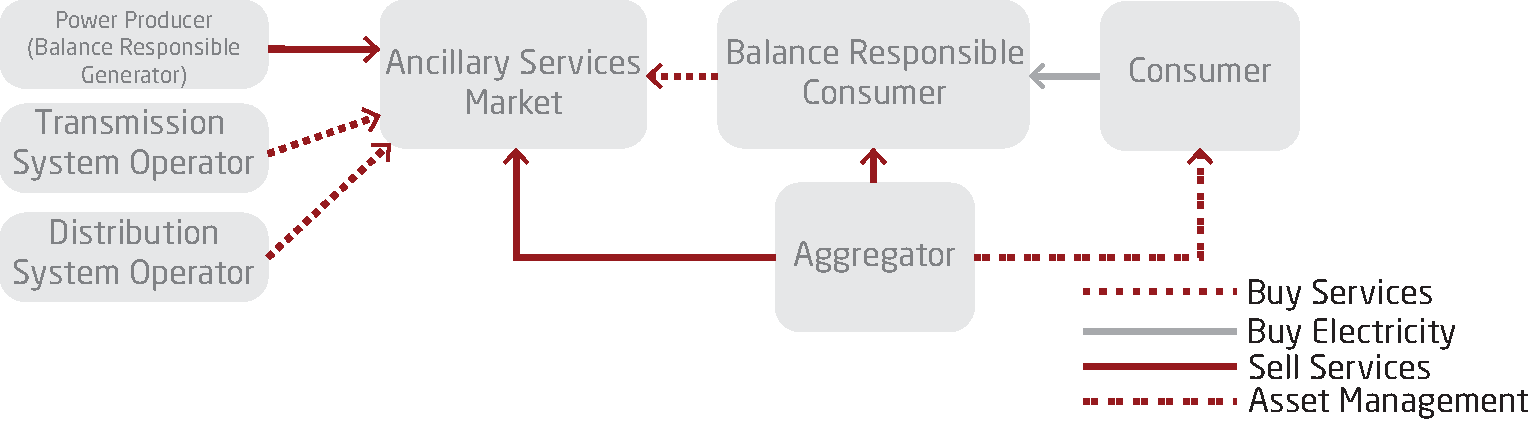
\includegraphics[width=\textwidth]{intro/market_future.eps}\label{fig:marketfuture}
\end{figure*}

In order to cope with the new problems, both at transmission and distribution level, it is expected that consumers will become prosumers. That is, the consumers will take an active role in the power markets by selling services to the system operators through an aggregator\footnote{The concept of the aggregator is introduced here, and is discussed in depth in Chapter~\ref{cha:aggregator}.}. The aggregator will provide an asset management service to the end consumer, and by managing a pool of consumers, it will be able to control a large enough consumption volume to provide ancillary services to the System Operators, or balancing services to the consumption BRP. The action of a consumer changing his or her consumption based upon an incentive is known as Demand Response (DR). The Aggregator facilitates DR by providing the ICT infrastructure and control infrastructure to DER owners, as well as statistical certainty of service delivery and legal responsibility towards the System Operators. The Aggregator can be an independent commercial entity, or it can be a function inside one of the pre-existing market players. The new market setup can be seen in Fig.~\ref{fig:marketfuture}, and it shows how the Aggregator player will interact with the existing market setup, and how the DSO will become a new player in the market, which will acquire ancillary services to resolve some of it problems.

In conclusion, we see the electric power system moving away from a \emph{production-must-follow-consumption} pattern to \emph{consumption-should-partly-follow-consumption} and hereby facilitate the integration of renewables and DERs. An integral part of achieving this change will be the use of control services to change the consumption behavior of units in the network. Given that the units providing ancillary services to the grid are critical for the security of the system, the new control algorithms and infrastructure must be validated.



\todo{amplify the paper to contain an analogy of the frequency as inflow and outflow of a water tank}
% section Short introduction to the power system (end)

\section{Problem statement, Delimitation and Contributions} % (fold)
\label{sec:Funneling}
\newsection{W}{hat is meant by} control-services? This is a broad definition, and here I will  narrow down my research to use control services to provide ancillary services, primarily through demand response, but the techniques should be able to be generalized.

Scoping of the PhD, and what the rest of the thesis will contain.

This thesis draws upon concepts from different fields and is multidisciplinary in its approach. Concepts from:
\begin{itemize}
	\item Power systems engineering
	\item Control engineering
	\item Software engineering
	\item Systems engineering
	\item Energy policy and regulation
\end{itemize}

What is meant with control services? In european context it is very much focused on Ancillary Services, while in the US Demand Response has not been used very much as AS, but rather used by ISOs as a mechanic to cope with peak consumption, or in the wholesale market. In the US context it would not make sense to call the upward service for the aggregator an ancillary service. Maybe aggregator business case?

Three kinds of stability: rotor angle, frequency stability and voltage stability[maybe cite kundur here?]. This work focuses on frequency stability, although there has been done some brief work on voltage issues in Xue's paper. 

``futures necessarily be- long to the present: they are what we imagine for ourselves now. The present is itself only made visible against a past''[cite: Marilyn Strathern, 1992]

Product Delivery: Performance Measurement 
Performance measurement, which is typically termed Measurement and Verification (M\&V), is the process of quantifying and validating the provision of the service according to the specifications of product. The performance measurement process usually occurs at three stages: 
\begin{itemize}
	\item To qualify potential resources against product specifications as an entry gate to participation 
	\item To verify resource conformance to the product specifications during and after participation 
	\item To calculate the amount of product delivered by the resource as part of financial settlements
\end{itemize}
 
All resources should be held to the performance specifications established by the product. However – demand side and generation side communication requirements will usually need to be designed separately and made appropriate to each. Technical rules often proscribe the use of metered values to base performance and settlements.[from the SEDC report used in the DRAS paper]

% section Funneling (end)



%%!TEX root = ../Thesis.tex
\chapter{Background} % (fold)
\label{cha:background}
Here goes everything related to the ``literature study''. Focus will be on ancillary services and demand response. What are the barriers for DR in the current markets. Part of this section will come from the paper on Redefining Ancillary Services for Technology Agnostic Sources.
% chapter Background (end)


%!TEX root = ../Thesis.tex
\chapter{The Aggregator} % (fold)
\label{cha:aggregator}
Introduce concept of fragility as described by Nassim Taleb. Look up Black Swan\ldots
The Aggregator
\begin{itemize}
	\item Aggregator Reference Architecture
	\item What can we test, and what should be tested?
\end{itemize}
% chapter The Aggregator (end)

%!EX root = ../Thesis.tex
\chapter{Validation of Aggregators}
\label{cha:validation}
\newchapter{I}{t is expected that} aggregators of large quantities of flexible consumption or production units will be able to provide ancillary services to TSOs and DSOs, as well as other flexibility services, \eg portfolio balancing for BRPs. Since the provision of ancillary services is essential for the security of the power system, units providing these services must go through a prequalification process by the appropriate entity. This could be the TSO\footnote{In Denmark, Energinet.dk is the TSO and is in charge of the prequalification/approval process (described in \cite{EnerginetAncillary}).}, a DSO or even an independent third party\footnote{For the rest of this chapter the responsible for carrying out the aggregator validation will be called the \emph{testing entity}.}. Traditionally, the prequalification process in Denmark has consisted of an initial submission of documentation describing the capabilities of the unit, and subsequently a test that validates the unit capabilities and communication. While this validation test is well established for large central generation units, how the test is to be applied to aggregators is still an open question. The solution to this question is of utmost importance if aggregators are to deliver ancillary services. In Chapter~\ref{cha:aggregator} the essential differences between aggregators and traditional generators are mentioned. In this chapter, these differences are expanded upon, and a novel method for aggregator validation is presented. Furthermore, one of the main contributions of this work is the exploration in the alignment between service requirements and the tests required to validate aggregators. These concepts are originally presented in the conference paper\fcite{bondy2016validation} which can be found in Appendix~\ref{app:pscc2016}. The presented validation framework is original to this work. The validation process described here focuses on aggregator providing ancillary services, but can also be applied as a certification method for aggregators, such that they can participate with other products in the electricity market.

\section{Background}
\newsection{S}{ince ancillary services are} essential for the reliability of the power system, units that provide said services must have a high degree of reliability. The TSO requires units that provide ancillary services to pass a prequalification process. This prequalification process consists of validating the unit for service delivery. In this section conventional resource validation is briefly discussed and it is explained why the same method can not be applied to aggregators. Also a short section on the current work on aggregator testing is presented.
\subsection{Conventional Resource Validation vs. Aggregator Validation}\label{subsec:backgroundvalidation}
In Denmark, the prequalification\marginnote{The topic of conventional resource validation is discussed in more detail in Section~\ref{sec:PSSCCconventionalvalidation}.} process is divided into two steps:
\begin{enumerate}
	\item documentation for the unit is submitted to the TSO, and
	\item a test procedure where the unit response to a signal from the TSO is evaluated.
\end{enumerate}

The unit response tests serves two purposes: it validates that the response corresponds to the presented documentation, and it tests the communication system between the TSO control room and unit. If the units succeeds in the prequalification process, it is certified for participation in the ancillary service markets.

This process works on traditional generators because the dynamics of traditional generators are well understood. That is, generators can be described to a large degree of certainty through physical equations, and the unit response test serves to confirm the documented values of the equation variables\footnote{The response test can also be seen as a system identification test.}. This is not possible for aggregators because they behave fundamentally different from large generation units:
\begin{enumerate}
	\item The aggregator portfolio can either be of a heterogeneous or homogeneous nature. \marginnote{A homogeneous aggregator is one which has a portfolio of same units, \eg a fleet of EVs. A heterogeneous aggregator has a mix of units in its portfolio, \eg EVs and thermostatically controlled loads.}In both instances, the variance of the response of the portfolio units, along with the tynamic nature of the portfolio, means that the aggregator can not be described through physical equations and a single response test will give no insight to the overall response capabilities of the aggregator. This is aggravated by the fact that each DER will have its own set of requirements to satisfy its owner's needs.
	\item Since the aggregator consists of geographically dispersed units, there is no single point of measurement. This means that the aggregated power profile does not represent a measurement at any single point in the power grid. This also means that traditional measurement systems can not be used on aggregators.
	\item The reliability concepts for distributed systems are different than those of single large units. Specifically, the failure modes are very different. The failure in a single unit in the aggregator has a much smaller impact on the overall aggregator performance compared to the failure of a subsystem in a generator fails.
	\item Aggregator architectures will vary widely, and may be respond differently depending on the grid state, weather conditions and user behavior. An aggregator must be tested for a variety of operating conditions which are irrelevant for traditional generators.
	\item Aggregator do not necessarily have a production or consumption baseline base upon operational schedules. This creates the challenge of determining if a service provided by an aggregator will effectively help the system, or is the aggregator being paid for a schedule it would have executed regardless. Also, this issue with the baseline means that without proper policy, the aggregators could introduce problems to the system and then be paid to solve them.\todo{Check if the points more or less match the corresponding from the previous chapter}
\end{enumerate}

It is both impractical and meaningless to validate every unit in an aggregator portfolio. The aggregator architecture must be tested as a whole, based upon statistical methods.

\subsection{Aggregator Testing in Literature}\label{subsec:aggtest}
There is currently no standardized procedure for prequalification of aggregators as there is with traditional generation units. Until now, the performance evaluation and testing of aggregators in academia has been ad-hoc to specific aggregator implementation\fcite{vrettos2015integrating}, or the evaluation focus has been on computational or financial performance\fcite{su2012performance,rahnama2014evaluation}. Similarly, a platform for simulation of aggregation strategy has been proposed\fcite{dittawit2014demand}, but the focus is on the simulation tool itself, which in turn focuses only on the demand side, and not on the process of validation. None have taken a systematic approach to generally evaluating the performance of the aggregators in terms of the contractual requirements of service delivery.

%\begin{itemize}
%	\item What is the control services validation problem, and why is it important?
%	\item What is the general framework I propose?
%	\item Which are the components in this framework that I have worked on?
%\end{itemize}

\section{The Validation Framework}

\newsection{T}{he definition of a} standardized validation procedure will become relevant as more aggregators, with a variety of architectures, appear in the power system and are willing to participate in the ancillary service markets. The process of validation for aggregators has three motivations: 
\begin{itemize}
	\item Allowing System Operators to contract aggregators that are able to provide adequate services (similar to the prequalification process that current generators must undergo) by documenting the reliability of the aggregators.
	\item Ensuring balance responsible parties or other entities seeking to contract flexibility services that the aggregators are capable of reliably delivering electricity products.
	\item Allowing commercial entities interested in entering the aggregator market to test the design of their aggregator infrastructure and control algorithm before deployment.
\end{itemize}

The reliability of the aggregator depends on stochastic processes, \eg consumer patterns and weather behavior. Therefore, it is natural that the validation procedure gives a statistical measure for the reliability. This means that the aggregator must undergo a series of validation test cases, as depicted in Figure~\ref{fig:MAINframework}. Formulating a set of test scenarios constrains the testing of the aggregator to a set of circumstances that the aggregator is expected to be able to handle, see Figure~\ref{fig:aggstatespace}. These kinds of tests must to be reproducible and with sufficient sampling so that the validation can be backed up with statistical certainty. It is infeasible to carry out this procedure the physical system. Therefore, this test process has to be carried out with aid of detailed simulations of the aggregator interaction with the electric power system and DERs, in combination with general models for communication.
\begin{figure}[htbp!]
\centering
\includegraphics[width=0.7\textwidth]{validationMAIN.eps}
\caption{Schematic process for aggregator validation.}
\label{fig:MAINframework}
\end{figure}

\begin{figure}[htpb!]
\centering
\includegraphics[width=0.8\textwidth]{aggstatespace.eps}
\caption{From all the possible state space the aggregator can operate in, it is only a subset that is considered nominal operation. Within this nominal operation, a test operation space is defined, where the stochastic variables that affect the aggregator performance are manipulated to test the aggregator reliability. These stochastic variables include, but are not limited to, weather conditions, communication failure and user behavior.}
\label{fig:aggstatespace}
\end{figure}

The proposed simulation tests should be carried out within a validation framework, as depicted in Figure~\ref{fig:frameworkbig}. The service requirements describe the goal the aggregator needs to achieve and the test scenarios define the normal operation disturbances that an aggregator should handle. The aggregator will not be held responsible for service non-delivery when it is affected by major problems outside its responsibility domain, \eg in case of severe grid faults. The service requirements are discussed in depth in Chapter~\ref{cha:services} and the service verification and evaluation is discussed in depth in Chapter~\ref{cha:verification}.

\begin{figure}[ht]
	\centering
	\caption{The validation framework, where the aggregator is the unit-to-test, is ideally composed of a software co-simulation platform with hardware-in-the-loop capabilities. The inputs are the validation test cases, and the output (\ie the service) is verified and evaluated. The arrows represent information exchange.}
	\includegraphics[width=\textwidth]{framework/framework.eps}\label{fig:frameworkbig}
\end{figure}

\section{Procedure for Validation of Aggregators} 
\newsection{F}{rom the previous} section it is clear that the service requirements form an essential part of the aggregator validation process. Service requirements are discussed in the depth in Chapter~\ref{cha:services}, but a set of test service requirement metrics have been formulated as part of the test method and are presented here.

\todo{include the Design of Experiments stuff from the pscc paper}

In order to measure how disturbances\footnote{See Figure~\ref{sec:servreqmet} for a visual representation of how disturbances affect the aggregator} affect service delivery, a set of performance metrics must defined. Based upon the current ancillary service definition, the chosen metrics are:
\begin{description}
	\item[Time responsiveness:] how fast can the service be delivered from the moment the reference or measurement signal changes.
	\item[Grid responsiveness:] how well can the aggregator follow changes in the grid state.
	\item[Response accuracy:] how good is the aggregator at providing the full volume that is requested.
\end{description}

It is the TSO that defines the value of these metrics that signify a passed validation test. Since the tests are stochastic, the metric value should also have a stochastic component, this could for example be \emph{time responsiveness} of service provision of 5 seconds with variance of $\pm$ 1 second. The metrics must be measured by an index and while literature has a wide array of indices for measuring performance, a specific index for aggregators is presented in Chapter~\ref{cha:verification}.

In order to align the service requirements and the test design, the following steps are proposed:
\begin{enumerate}
	\item The aggregator informs of the general composition of its portfolio, as well as the service it wants to be validated for.
	\item The tester identifies the appropriate service requirements for the service to be tested for.
	\item The tester identifies the expected normal operation of the aggregator.
	\item The tester defines the test operation scenarios that the aggregator is expected to perform under. The scenarios must define the statistical properties, \eg mean and variance, for the stochastic disturbances affecting the aggregator performance.
	\item The tests are carried out on the aggregator.
	\item The aggregator performance is evaluated.	
\end{enumerate}

Note that the entity performing the validation tests can be an independent party, \eg a third party certifier for aggregators, or it can be the TSO.

Depending on the excitation signals the aggregator is subject to, the tests are divided into two categories:
\begin{itemize}
	\item step response, and
	\item continuous reference tracking.
\end{itemize}
The kind of test used for the validation will depend on the test scenario description.

\section{On Prequalification and Certification of Aggregators}\label{sec:aggpreq}
\newsection{I}{t was previously mentioned} that traditional generator prequalification consists of two steps, the documentation of the generator and the response test. In Chapter~\ref{cha:aggregator} a functional reference framework for aggregators was introduced. This reference architecture can be used as a checklist, along with the test results from the validation framework as the documentation part of the prequalification of aggregators. A response test should be performed, not to validate the aggregator reliability, but to verify the communication between the TSO control center and the aggregator. Furthermore, aggregator performance should be continually evaluated, and new validation tests should be carried out routinely. This is due to the dynamic nature of the aggregator portfolio, which may regularly change in size and composition.

\section{Conclusions Regarding the Validation Framework}
\newsection{T}{he concept of validation} of aggregators is important for the participation of aggregators in both ancillary services markets and energy markets. The original contribution of this work is the design of the aggregator validation framework and specially the analysis of aligning service requirements with test design. The described approach to test the system through statistical methods and define the requirements as with statistical values is novel.

A weakness in the proposed method is that the validation tests are highly dependable on the accuracy of the used models in the simulation. A way to mitigate this is to make the framework modular so that the tests can be run with hardware-in-the-loop (for model validation of individual units) or so that the framework can be connected to validated models, \eg a Real-Time Digital Simulator (RTDS). 

Future work will consist of further refining the validation architecture, specifically defining the interfaces between modules, and implementing the software platform.

%!TEX root = ../Thesis.tex
\chapter{Service Modeling and Requirements} % (fold)
\label{cha:services}
\begin{marginfigure}
	\includegraphics[width=\textwidth]{framework_services.eps}
	\caption{This chapter focuses on the \emph{service definition} block of the aggregator validation framework presented in Chapter~\ref{cha:validation}.}
      \label{fig:framework_services}
\end{marginfigure}

\newchapter{T}{he requirements for ancillary} services in many countries are defined, due to historical reasons, on the assumption that only generators provide ancillary services. It is clear that current service requirements in many countries are directly, or indirectly, blocking the integration of aggregators providing DR\fcite{cappers2013assessment,coalition2014mapping}. If aggregators are to be successfully integrated into the power system, the rules and requirements for participation must be changed. This chapter presents two novel contributions to integrating aggregators in the power system: a modeling method for services, and a proposal for the restructuring of requirements for ancillary services. A method for modeling services is important because the resulting models form the benchmark for the performance evaluation and verification of the aggregator (see Chapter~\ref{cha:verification}), as well as being a direct input to the aggregator (see Chapter~\ref{cha:aggregator}). The redefinition of ancillary service requirements is important since it will allow system operators to utilize the properties of all available resources, both traditional and new, in an optimal way. 

The concepts presented in this section are part of two draft journal papers\fcite{bondy2016method,bondy2016redefining} which can be found in Appendix~\ref{app:segan} and Appendix~\todo{Berkeley Ref}, as well as work done as a collaborating author for a conference paper\fcite{heussen2013a} and a technical report written for the iPower consortium\fcite{bondy2014flech}. Section~\ref{sec:backgroundservicesandreq} discusses different kinds of services that aggregators can provide and Section~\ref{sec:modelingAS} presents how these can be modeled. These models are directly related to the \emph{service requirements} block in the aggregator validation framework (see Figure~\ref{fig:framework_services}). In Section~\ref{sec:RedefiningAncillaryServiceRequirements} a proposal for how ancillary service requirements can be reformulated in order to be technology agnostic. 

%Content of this chapter is the work done at LBNL and through the iPower demo.
%\begin{itemize}
%	\item Service definition
%	\item What are aggregators expected to deliver?
%	\item PowerMax service requirements
%	\item Redefining Ancillary Services Requirements for Technology Agnostic Resources
%\end{itemize}

\section{Background}\label{sec:backgroundservicesandreq} % (fold)
\newsection{T}{he following section outlines} concepts related to the definition and requirements of services at TSO and DSO level. While services for the TSO (ancillary services) are well established, DSO services are a relatively new concept which has been explored in iPower project\fcite{ipower2013development}.
\subsection{What are Ancillary Services?} % (fold)
\label{sub:ancillaryservicesdef}
Defining what \gls{as} are, as well as which services the term includes, is difficult. This is due to both the differences in the way power systems are managed around the world and the differences in the terminology used to refer to such services. There is overlap between the European and US definition\fcite{eurelectric2004,ferc1997} of AS in that both describe them as services used to ensure the reliability of the power system. In both European and US context reliability is addressed by considering \emph{system adequacy} and \emph{security} \footnote{NERC also used the term system security, but in September 2001 security became synonymous with homeland protection in the US. Now it uses the term \emph{operating reliability} \cite{nerc2007definition}}. \emph{System adequacy} is the power system's ability to supply the electricity demand at all times and \emph{security} is the ability to withstand sudden disturbances.

Generally, maintaining an adequate and secure power system means maintaining the power system operating at nominal frequency and voltage. In cases where the power system deviates from nominal operation, either due to natural fluctuations in production/consumption or faults in the system, the system operators will activate ancillary services to restore normal operation. 

Some countries, \eg Denmark, consider voltage control, black start capabilities, short circuit control and reactive reserves as AS. This work focuses on those services that use active power to maintain the nominal frequency of the grid. In Europe\footnote{ENTSO-E changed in 2013 its nomenclature of AS, and the three presented here correspond roughly to the classical primary, secondary and tertiary reserves as presented in \cite{Rebours}.} these services are \glspl{fcr}, \glspl{frr} (either automatic\footnote{In the United States, regulation is used for system balancing. This service corresponds to automatic FRR.} or manual), and \glspl{rr}\fcite{entsoe2013network}.

These reserves are activated as illustrated in Figure~\ref{fig:MAINfreqcont}. The FCR is the fastest reserve and reacts automatically upon the grid measurements. Its role is to stop frequency excursions and its effectiveness can be measured by the \emph{frequency nadir} \cite{eto2010use}. The FRR is activated by tracking the \gls{agc} signal, or through manual activation by the system operator, relieves the FCR (allowing the FCR to be available again) and restores the frequency to the nominal value. The RR relieve the FRR, usually through rescheduling of units or by bringing inactive units online.

\begin{figure}[htbp!]
\centering
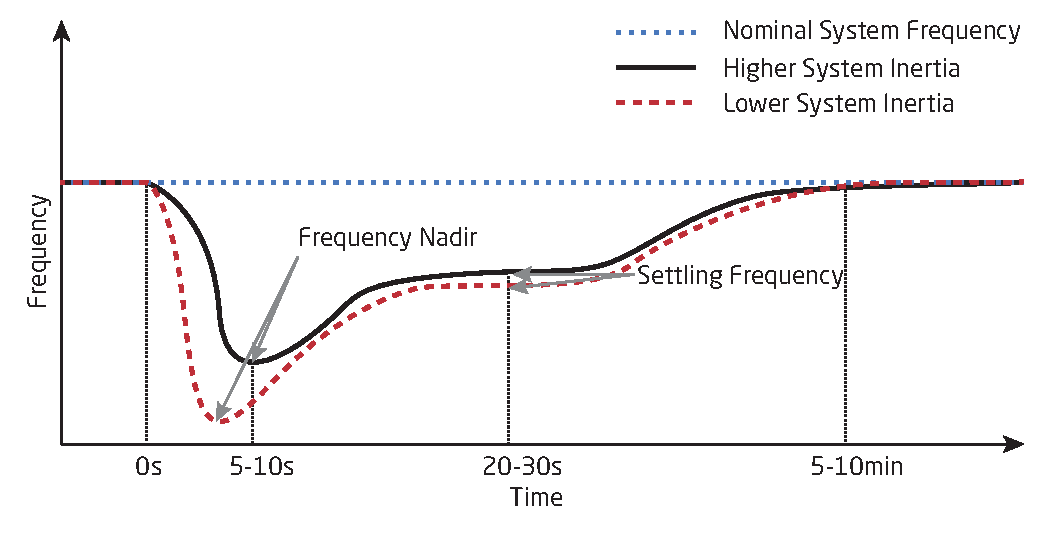
\includegraphics[width=0.9\textwidth]{frequency_contingency.eps}
\caption{The ancillary services are activated sequentially after a frequency contingency. In systems with high inertia the frequency nadir will occur at frequencies closer to the nominal frequency.}
\label{fig:MAINfreqcont}
\end{figure}

% subsection What are Ancillary Services? (end)
\subsection{Requirements for Ancillary Services} % (fold)
\label{sub:servreqAS}
Because AS are essential for the secure operation of the system, the system operators have requirements and restrictions on the units providing AS. A super-set of requirements across different systems was presented by \emph{Rebours}\fcite{Rebours}, and following his overview we classify requirements into three categories:
\begin{description}
	\item[temporal requirements] which relate to how fast and for how long a service must be delivered;
	\item[resource tuning requirements] which relate to specific values that tuning parameters in the resource must have;
	\item[market requirements] which relate to bid sizes and similar parameters in systems where services are acquired through market mechanisms.
\end{description}

Of these three categories, only the temporal requirements relate to service performance. Furthermore, in most systems, the requirements are implicitly defined for traditional generation units. This means that most service requirements are oriented towards the least common denominator of service providers, e.g. a unit providing FCR should provide half of the service within 15 seconds and full response within 30 seconds\fcite{EnerginetAncillary}. A variety of generation and consumption units would be able to provide this service faster, but this quality is not rewarded. Another example is the requirement of having a PI-controller on units providing FRR in order to track the AGC signal. Such a controller is infeasible on distributed systems, but other modern controllers can provide offset-free control with similar properties. This means that the historical requirements for units participating in AS markets in many countries act implicitly, or explicitly, as barriers for new technologies to enter the market\fcite{cappers2013assessment,coalition2014mapping}.%\todo{should I put in a more thorough description of FCR, FRR and RR, like what we have in the DDRAS paper?}

The concept of using demand side management to help the secure operation of the power grid has existed in different forms since the late 1970s\fcite{lampropoulos2013history}. But in recent years, the introduction of new consumption and generation technologies, \ie DERs, along with the roll-out of a smart metering infrastructure and the advances in ICT, has lead to the new opportunities in using smart control of small scale consumption/production as a service to the power grid. There is a large body of literature\fcite{oconnell2014benefits} concerning DR, and proposals to use it for AS\fcite{vrettos2015integrating,mathieu2012using,zarogiannis2014dynamic}.%\clearpage
% subsection Service Requirements for Ancillary Services (end)
\subsection{Distribution System Services} % (fold)
\label{sub:dsoservices}
As the amount of DERs installed at distribution level increases, the DSOs face new operational problems. Mainly, the increase in electric load will cause congestion and voltage issues. The traditional way of handling these are through reinforcement of the grid assets. Given the high cost of installing new cables, and the uncertainty in how the electricity consumption will change in the future, the use of flexibility services will be an attractive alternative.

One of the main outcomes of the iPower project was the definition of a set of flexibility services that demand aggregators can provide DSOs\fcite{ipower2013development} for congestion management or voltage issues. The requirements for three of the congestion management services have been further detailed individually\footnote{The services requirements were detailed in the following technical reports\cite{hansen2013flech,biegel2014flech,bondy2014flech}.}, and aggregator architectures have been designed to provide both congestion management\fcite{hu2014coordinated} and voltage support\fcite{han2014assessment}. At the same time, the concept of the \gls{flech} has been designed as a platform to enable the transparent contracting of flexibility\fcite{heussen2013a}.

An example of a flexibility service is the \emph{PowerMax}\fcite{bondy2014flech} service, where the aggregator maintains the total consumption of its portfolio under a limit, within a specified period of time. This means that the aggregator is free to manipulate its portfolio as long as its peak load is below the limit specified by the DSO.
% subsection DSO Services (end)
\subsection{Asset Management Services} % (fold)
\label{sub:assetmanagementservices}
In Chapter~\ref{cha:aggregator} the concept of \gls{ams} is introduced as the services that an aggregator provides to the owner of the DERs, or flexibility assets. An example of this is the case where the aggregator is an EV fleet operator that has the contractual responsibility of maintaining all EVs in the fleet within a certain \gls{soc}. The purpose of validating aggregators for these services is that flexibility asset owners can use the validation as a trust measure.

The main idea behind AMS is that the flexibility assets have a primary purpose, which is to satisfy the needs of their owner. The aggregator can use the flexibility of the units as long as the primary purpose is respected. Thus, from the perspective of customer comfort, an aggregator that is better at AMS is more desirable. 
% subsection Asset Management Servc (end)
% section Background on Aggregator Services (end)
\section{Modeling of Service Requirements} % (fold)
\label{sec:modelingAS}
\newsection{T}{he validation framework} presented in Chapter~\ref{cha:validation} uses the \emph{service requirements} as a benchmark towards which the aggregator is evaluated. This is because the requirements form the control objective of the aggregator. Currently, requirements for services are encoded within the contractual agreements between system operator and service provider. A standard method is needed for extracting this information and building a model that can be used for benchmarking.

By analysing the services presented in Section~\ref{sec:backgroundservicesandreq}, a method for translating the contracts into a time series model has been developed. The method consists of the following six steps:
%form have been identified as a generic method for modeling ancillary services. The steps are exemplified by DSO services defined in  and TSO services defined in :
\begin{enumerate}
  \item Identify physical parameters defining the service.
  \begin{itemize}
    \item \eg Power production or consumption, measured grid frequency, time measurements, etc.% Including maximum measuring sensitivities.
  \end{itemize}
  \item Identify the dynamic behaviors of the service related to system parameters (if any).
  \begin{itemize}
    \item \eg FCR expects a linear relation between a deviation from the nominal grid frequency and the generator set-point.% Power-cap has a dynamic relationship between feeder load and the controllable load power in order to keep the total feeder load at a $P_{DSO,Ref}$ value.
    %\item PowerMax is not dynamic. The aggregator must control $\Delta P_{Agg}$ to ensure that he does not violate $P_{max,Agg}$. But the service does not require a dynamic behavior related to a system parameter like primary frequency regulation and PowerCap.
  \end{itemize}
  \item Identify the physical size of the service and the tolerated error. % Both ideal service and minimum required service.
  \begin{itemize}
    \item \eg the volume of the bid for FCR. %Physical size is for example $P_{max,Agg}$ for PowerMax service or
%    \item Tolerance is for example $P_{max,Agg}+P_{tolerance}$ for the PowerMax service and allowed dead-band for DK1 primary reserve.
  \end{itemize}
  \item Identify the ideal response time of the service and acceptable response.
  \begin{itemize}
%    \item Most contracts comes with some timing specifying how fast the service provider must act.
    \item \eg FCR in western Denmark must be 50 \% of activated within 15 s and 100 \% within 30 s.
%    \item The ideal service is for example an instantaneous step in power to 100 \% of set-point for DK1 primary reserve.
  \end{itemize}
  \item Based on the dynamics, size and timing of the service, as well as the tolerated errors from points 1--4, develop a time series for ideal and acceptable service provision. The model will be a set of time series: $\mathbf{x}_{ideal}(t)$ for ideal response and $\mathbf{x}_{acc}(t)$ for acceptable response. Both time series can be a scalar or a vector, e.g. $\mathbf{x}_{acc}(t)$ can be formed by a set of upper and lower tolerance bounds or simply by an upper bound.
  \item Identify how the service error is to be measured.
\end{enumerate}

  %§$\mathbf{x}_{ideal}(t)$ and $\mathbf{x}_{acc}(t)$ can be a pair of values, e.g. minimum and maximum tolerance limits, for some services and may be only a single value, e.g. minimum or maximum tolerance, for others. 
Furthermore, the analysed services can be divided into three kinds of services:
\begin{description}
	\item[Reference Tracking:] Services where a reference signal must be followed, \eg regulation in the United States.
	\item[Band Service:] Services where the output is able vary between an upper and lower limit, \eg smart charging of a fleet of EVs.
	\item[Cap Service:] Services where the output must respect either a upper or lower bound, \eg the \emph{PowerMax} service.
\end{description}

Based upon the three kinds of service, the service error can be measured the following ways:
\subsection*{Reference tracking}

Reference tracking error can be calculated as:
\begin{equation}\label{MAINeq:ref_error}
e(t) = x_{meas}(t) - x_{ideal}(t),
\end{equation}
\begin{marginfigure}
	\includegraphics[width=\textwidth]{tracking_error2.eps}
	\caption{Error in reference tracking.}
      \label{fig:reftrackerrorMAIN}
\end{marginfigure}
where $x_{meas}(t)$ is the measured output, \eg the total load of the aggregator portfolio, and $x_{ideal}(t)$ is the ideal response defined in the service model. This definition will lead $e<0$ for measured values below the ideal and $e>0$ for values above the ideal. In this case $\mathbf{x}_{acc}(t)$ will be a band around $x_{ideal}(t)$, and the values of $\mathbf{x}_{acc}(t)$ do not need to be symmetric.

\subsection*{Band service}
The ideal response in a band service is defined as $ \mathbf{x}_{ideal}(t)= [x_{min}(t),x_{max}(t)]$. The error in the band service can therefore be estimated by:
\begin{equation}\label{MAINeq:band_error}
e(t)=
\begin{cases}
x_{meas}(t) - x_{min}(t) , & x_{meas}(t) < x_{min}(t)  \\
0, & x_{min}(t) \leq x_{meas}(t) \leq x_{max}(t) \\
x_{meas}(t) - x_{max}(t), & x_{meas}(t)  > x_{max}(t).  
\end{cases}
\end{equation}
\begin{marginfigure}
	\includegraphics[width=\textwidth]{band_error2.eps}
	\caption{Error in band service.}
      \label{fig:banderrorMAIN}
\end{marginfigure}

In this case, the $\mathbf{x}_{acc}(t)$ is a set of values that surrounds the band defined by $ \mathbf{x}_{ideal}(t)$, as seen in Fig.~\ref{fig:RefErr}. The values of $\mathbf{x}_{acc}(t)$ do not need to be symmetric around the band.

\subsection*{Cap service}
%Maximum/minimum cap error only counts the error when performance is above/below some ideal value. 
In cap services, error is only tracked when $x_{meas}(t)$ is either above or below a given a limit value.
Maximum cap error is calculated as shown in \eqref{MAINeq:maxmin_cap} and minimum cap can be similarly calculated. In \eqref{MAINeq:maxmin_cap}, $x_{max}(t)$ is the ideal maximum limit according to the service contract:

\begin{equation}\label{MAINeq:maxmin_cap}
e(t)=
\begin{cases}
x_{meas}(t)-x_{max}(t), & x_{meas}(t) > x_{max}(t) \\
0, & x_{meas}(t) \leq x_{max}(t).
\end{cases}
\end{equation}
\begin{marginfigure}
	\includegraphics[width=\textwidth]{cap_error2.eps}
	\caption{Error in cap service.}
      \label{fig:caperrorMAIN}
\end{marginfigure}

In the cap service, $x_{acc}(t)$ is a limit that either lies below $x_{min}(t)$ or above $x_{max}(t)$.


% section Modeling of Ancillary Services (end)

%
\section{Restructuring Ancillary Service Requirements} % (fold)
\label{sec:RedefiningAncillaryServiceRequirements}
Until now, system operators have been able to arrest frequency excursions fast enough because of the inherent system inertia. With the increasing penetration of wind power in the system, the electricity prices are lowered and operating fossil-fueled generator becomes economically unfeasible. This has the effect of reducing the system inertia, and reducing the availability of AS resources. Therefore new AS sources with faster response times are required. \emph{Vrettos et al.}\cite{vrettos2015integrating} show that if FCR is provided by DR (with a very fast response), the frequency nadir occurs at higher frequencies.
Also, \emph{Makarov et al.}\cite{makarov2008assessing} argue that the value of regulation resources can be defined based upon the ramp capabilities of the service providing units. Faster reacting units are more valuable to system operators, since they help arrest the frequency excursion faster and at a higher nadir.% It does require changes to the AGC in order to utilize the fast response, but this would also lead to the need for fewer reserves.

AS requirements are specified by a system operator based on the desired control response for a particular power system, under the implicit assumption that the ideal unit response corresponds to a scalar fraction of the required system response. Today, these requirements --- as reflected in the service definition --- are not differentiated according to the capabilities of the unit providing the service. Therefore, service definitions are designed to accommodate the least capable unit in the portfolio. As a consequence, more capable units are not being fully utilized, leading to excess contracting of service providers.

 In this section a new form of defining AS requirements is presented, which has as an objective to allow all units to participate in the AS markets on equal footing. The main assumption is that all units can be valuable for AS provision, even when they do not fully comply with current requirements, and that the system operators will be able to manage the system better if the capabilities of all available resources are utilized. Also, units should be remunerated based upon the value they represent to the operation of the system, and their performance compared to these expected values.

Regulative authorities have concluded that fast reacting units are valuable for the system operation, and started programs to benefit of these resources. An example of this is FERC order 755 (Pay for Performance) which has led to PJM splitting their regulation market product into RegA, for slow reacting units, and RegD for fast reacting units. The product differentiation approach has been a success for PJM, but  splitting the market may still lead to suboptimal utilization of units and does not address the issue of new technologies being effectively excluded from certain markets.  We propose instead to restructure the ancillary service definitions such that all types of service providers participate with the same market product defined by a set of optimal performance parameters, and not by minimum requirements. This means that the all entities providing a given ancillary service are optimally cleared under a single market.

\subsection{The Overall Approach} % (fold)
\label{sub:TheOverallApproach}
The restructuring of AS requirements is formed by the following key concepts:
\begin{enumerate}
	\item The system operator is able to formulate an overall \emph{ideal AS response} that can be achieved through an optimal mix of resources. Any resource can make a bid for providing part of this ideal response.
	\item The \emph{parametrization of AS bid}, where the parameter values of each unit/bid reflect the service provider's capabilities to partially fulfill the ideal response. This avoids excluding units that may have useful capabilities in one parameter, e.g. very fast ramp rate, but low capabilities in another parameters, e.g. only holding the response for a short time. Such a service definition allows compliance to be measured on a linear rather than a binary scale: In addition to compliance and noncompliance, different levels of partial compliance are possible.
	\item Clearing all units under a \emph{generalized single clearing-price auction} allows constructing an optimal portfolio, and enables competition between all resources, leading to lower prices.
    \item \emph{Performance-based remuneration} gives incentive to better AS provision and enables transparent performance-based clearing of the market.
\end{enumerate}

These key concepts are discussed individually in the following subsections.
% subsection The Overall Approach (end)
\subsection{Ideal Service Tender} % (fold)
\label{sub:IdealServiceTender}
The ideal source for AS is one with ``unlimited capabilities in terms of response time, energy output, ability to frequently reverse their output, ability to respond and follow the AGC setpoint changes, and size .''\cite{makarov2008assessing}\footnote{For this kind of response to be optimal, changes must be made to the AGC algorithm \cite{peydayesh2012effects}.} It is impossible for any one unit to possess these characteristics, but system operators aim at achieving this kind of system response by contracting several units.

For example, a system operator could determine that the ideal system response to a frequency excursion is the one that has a resulting frequency nadir at the settling frequency (thus minimizing the risk of tripping the under-frequency relays). Based upon the inertia in its system, the system operator determines the volume ($V_{tot}$) needed as well as the response characteristics needed to achieve this, see Figure~\ref{fig:idealresponse}.

\begin{figure}[htbp!]
\centering
\includegraphics[width=0.9\columnwidth]{primary_frequency_control_ideal.eps}
\caption{In this case, the ramp of the ideal response is mainly determined by the system inertia and is to be sustained until FRR can be activated.}
\label{fig:idealresponse}
\end{figure}
% subsection Ideal Service Tender (end)
\subsection{Service Parametrization} % (fold)
\label{sub:ServiceParametrization}
The overall ideal service requirements can be expressed as:
\begin{equation}
	S^* = f_m(\textbf{x}^*) \label{eq:optimaltender}
\end{equation}
where $\textbf{x}^*$ is a vector of ideal parameter values and $f_m(\cdot)$ a function that translates the parameters $\textbf{x}$ into a model, e.g. into a time series as shown in Section~\ref{sec:modelingAS}. Furthermore, the system operator must inform how the parameters are valued with respect to the $S^*$, which is done through a capability value:
\begin{align}
    \kappa &= g(\mathbf{x}) \\
    \kappa &\in [0,1].
\end{align}

For example, a system operator decides that FCR in their market is defined by $\textbf{x} = [\tau_r,\tau_d,V]$, where $\tau_r$ is the rise time of the service, $\tau_d$ is the duration of the service, and $V$ is the volume of the service. Due to the properties in its system, it decides that $\textbf{x}^* = [30 s, 20 min, 90 MW]$. The capability value of each bidder is calculated by:
\begin{equation}
	\kappa_i = \alpha_1 \frac{\tau_{r,0}}{\max({\tau_{r,0},\tau_{r,i})}} + \alpha_2  \frac{\min(\tau_{d,0},\tau_{d,i})}{\tau_{d,0}} + \alpha_3 \frac{V_i}{V_{tot}}, \quad \forall \, i \in \Omega \label{eq:kappa_primfreq}
\end{equation}
where $\tau_{r,0}$ and $\tau_{d,0}$ are a nominal value the system operator sets, $\tau_{r,i}$ and $\tau_{d,i}$ are the actual parameter values for each bidder, $\frac{V_i}{V_{tot}}$ is the bid contribution to the total required volume, and $\Omega$ is the pool of bids. Finally, $\sum_{i} \alpha_i = 1$, and in this case could be $\alpha_1,\alpha_2 = \frac{2}{5}, \alpha_3 = \frac{1}{5}$.
% subsection Service Parametrization (end)

\subsection{Market Mechanism} % (fold)
\label{sub:MarketMechanism}
It is impossible to restructure the AS definition without addressing the market mechanism for determining the optimal set of resources. The market should be designed as a single clearing price auction, in which each resource bid is adjusted by \emph{two} factors for bid quality: 1) the capability value $\kappa_i$ and 2) a historical performance\footnote{The historical performance parameter can also be interpreted as an availability parameter, or certainty parameter.} parameter $\eta^{hist}_i$. In this section a proposal for how this market mechanism could be formulated is presented.

The proposed clearing mechanism identifies a common clearing price based on the most expensive accepted bid\footnote{This is similar to the merit order lists used in \eg the Nordic system for Manual Regulating Power\cite{bondy2013}.}:
%Clearing principles
\begin{equation}
    P^\mathtt{clear} = \max P^\mathtt{bid}_i, \quad i \in \Omega^\mathtt{acc}
\end{equation}
where $\Omega^{acc}\subseteq \Omega$ is the subset of accepted bids of the set of received bids $\Omega$. 
The clearing mechanism selects the subset of bids which offer the cheapest overall clearing cost and meet the tender requirements with a given certainty of availability: 
\begin{align}
      \Omega^\mathtt{acc} &= &\mathtt{argmin}_{\Omega^\mathtt{hyp} \in \mathcal P(\Omega)} \sum_{i\in \Omega^\mathtt{hyp}}{\kappa_i P^\mathtt{clear}_i } & \\
	  &\mathtt{s.t.}& \sum_{i\in \Omega^\mathtt{hyp}} f_m(\mathbf{x}) \geq S^* &  \\
      &~ & \eta^{hist}_i \geq \eta^{hist}_{min} &\quad \forall \, i \in \Omega^\mathtt{hyp} 
\end{align}
Where $\mathcal P(\Omega)$ denotes the Power Set of $\Omega$ and $\Omega^{hyp}$ is a subset of the Power Set. $S^*$ is the ideal tender from Eq.~\eqref{eq:optimaltender} and $\eta^{hist}_{min}$ is the minimum historical performance requirement to participate in the market\footnote{This value represents how averse the system operator is to risk, and could also be considered part of the service parameters $\textbf{x}$.}.

% subsection Market Mechanism (end)

\subsection{Performance Based Remuneration} % (fold)
\label{sub:PerformanceBasedRemuneration}

The estimation of the service provision performance can be done in different ways, depending on which parameters the system operator deems to be the most critical. The concept of performance assessment is discussed in Chapter~\ref{cha:verification}, and performance index is introduced there. Here it suffices to say that the performance measurement is a function of the error in service delivery:
\begin{align}
	\eta &= c(e(t)), \label{eq:perfindexsimple}\\
	\eta &\in [0,1]
\end{align}

We propose that remuneration is based on the performance evaluation of the service provision:
\begin{equation}
	P^\mathtt{rem}_i = \eta_i\kappa_i  P^\mathtt{clear} \qquad \forall \, i \in \Omega^\mathtt{acc}.
\end{equation}
Thus, remuneration is based upon the value the resource has to the grid operator, how well it performs, and the most expensive activated resource.
% subsection Performance Based Remuneration (end)

% section Redefining Ancillary Service Requirements (end)

\section{Conclusions on Service Requirements} % (fold)
\label{sec:ConclusionsServiceRequirements}
\newsection{A}{ggregators have become} possible sources for ancillary services and distribution system services. While system operators are aware of the potential in using flexibility for system balancing, the ancillary service requirements have not been changed in order to accommodate this new technology. This chapter presented a novel proposal for solving this issue, by restructuring the ancillary service requirements based upon a set of optimal parameters instead of the limiting minimum requirements found in many systems today.

Also, a method for modeling services was shown. The resulting models are relevant for the validation framework in that they provide the benchmark towards which aggregators must perform. In Chapter~\ref{cha:verification} it is shown how the service models can be used for performance assessment and verification of services.

The work presented in this chapter differs from the rest of the thesis, in that the concepts presented here are not focused on the aggregator itself. The service modeling method can be applied to any kind of service, not necessarily those provided by aggregators, and the objective of the ancillary service restructuring is to include any new technology, not only aggregators providing DR.

A final observation with respect to services is that operators like Energinet.dk are interested in acquiring flexibility from aggregators. The traditional approach to buying ancillary services is that the operator pays for an increase or decrease in power production, but flexibility has an extra dimension: time\footnote{See Chapter~\ref{cha:aggregator}.}. That is, flexibility is not only about increasing and decreasing production, but also about moving it in time. System operators expect flexibility services to fit in within the existing framework, but the two kinds of services can arguably be said to be essentially different. 

% section Conclusions on Service Requirements (end)
% chapter Service Requirements (end)

%!TEX root = ../Thesis.tex
\chapter{Verification of Aggregator Services} % (fold)
\label{cha:verification}

\begin{itemize}
	\item Why is verification an important part of validation?
	\item Performance Assessment of Aggregators providing Demand Response
\end{itemize}
% chapter Service Verification (end)


%\blinddocument
%!TEX root = ../Thesis.tex
\chapter{Conclusion and Future Work}
\label{cha:conclusion}
\newchapter{M}{orbi pharetra ligula} integer mollis mi nec neque ultrices vitae volutpat leo ullamcorper. In at tellus magna. Curabitur quis posuere purus. Cum sociis natoque penatibus et magnis dis parturient montes, nascetur ridiculus mus. Suspendisse tristique placerat feugiat. Aliquam vitae est at enim auctor ultrices eleifend a urna. Donec non tincidunt felis. Maecenas at suscipit orci.
\section{Discussion of key results} % (fold)
\label{sec:Discussionofkeyresults}


Aggregator validation consists of three things:
\begin{itemize}
	\item Documentation through the reference architecture
	\item Simulation aided validation tests
	\item Communication test
\end{itemize}

% section Discussion of key results (end)

\section{Future Work} % (fold)
\label{sec:FutureWork}

% section Future Work (end)

\section{Application} % (fold)
\label{sec:Application}

% section Application (end)


\appendix
\chapter{A Functional Reference Architecture for Aggregators}\label{app:etfa2015}

\textbf{Authors:}\\
	Daniel~Esteban~Morales~Bondy\\
	Kai~Heussen\\
	Oliver~Gehrke\\
	Anders~Thavlov

\noindent
\textbf{Published at:}\\
Emerging Technologies and Factory Automation (ETFA), 2015 IEEE\\
Luxembourg, Luxembourg

\noindent
	\textbf{Abstract:}\\
Aggregators are considered to be a key enabling technology for harvesting power system services from distributed energy resources (DER). As a precondition for more widespread use of aggregators in power systems, methods for comparing and validating aggregator designs must be established. This paper proposes a functional reference architecture for aggregators to address this requirement.


\section{Introduction}
\newchapter{T}{he} increase of electricity production from fluctuating renewable sources is creating a need for new ways of operating the power system. Demand response (DR), i.e. the exploitation of flexibility in electricity consumption, is considered a promising technology for mitigating this problem. However, a significant part of the DR potential exists in distributed, small and medium-sized loads. It is not practical for a power system operator to interact directly with all these flexibility assets. The role of aggregators is the creation and management of a portfolio of flexibility assets and  representation of this combined flexibility to a system operator and/or market.

System operators today rely on generators for ancillary services to maintain reliable system operation. Generators undergo validation tests and continuous monitoring on the generator site. With ancillary services provided by aggregators, similar validation and performance requirements will have to be established. However, validation and monitoring requirements cannot effectively be translated from single site monitoring to distributed aggregator control systems, and today's on-site monitoring cannot be scaled to distributed flexibility assets. 

We propose a functional aggregator reference architecture that facilitates specification and validation of aggregator functional requirements and the generic modeling of contractual and verification performance requirements. Application of the proposed functional architecture to  different aggregator designs suggests it as a meaningful benchmark for technology maturity.

% SUGGESTING TO REMOVE THIS PARAGRAPH FOR THE SHORT PAPER
%The paper presents a short overview of the current state of aggregation in Section~\ref{sec:agginsg}. The motivation for the reference architecture are presented in Section~\ref{sec:requirements} and an analysis of the aggregator functionality is presented in Section~\ref{sec:funcdec}. Section~\ref{sec:refarch} presents the proposed framework based upon the functionality analysis, and Section~\ref{sec:applic} shows how the framework can be applied to a set of academic and commercial aggregators.

%usual blabla about Smart Grids, and which problems aggregators are supposed to address in the Smart Grid context (scalability/divide-and-conquer, threshold to market entry, competition and indirectly robustness because of multiple implementations etc.). 
%\begin{itemize}
%\item Commercial aggregators are being developed by multiple parties and see their first field use. All of these are one-off designs.
%\item Performance evaluation and service validation will become important issues to be solved once aggregators are supposed to leave the protected field test environment and enter a competitive market.
%\item However, the wealth of different designs and solutions makes finding a common benchmark for evaluation and validation difficult.
%\end{itemize}
%This paper proposes a generic reference architecture for the performance evaluation of aggregators which can be used for ... and makes ... easier.

%Also, this work can serve as a checklist for companies that seek to start an aggregator business.
%Aggregation of large quantities of small, medium sized loads or a few large loads is a solution for harnessing resources that are useful for maintaining power quality and reliability in power systems with large penetration of fluctuating renewable energy sources.

%#############################################
\section{Aggregation in Smart Grids}
\label{sec:agginsg}
%This is where the state of the art goes:
%\begin{itemize}
%\item what is aggregation in a smart grid context?
%\item What is being aggregated?
%\item What is the purpose of the aggregation (delivery of which product?) 
%\item Which types of design exist (examples, not categorisation yet - we'll do that later) Examples
%\item Outcome: Why are aggregators an issue in smart grids?
%\end{itemize}
We refer to the concept of aggregation as the  creation and (commercial and technical) management of a portfolio of flexibility assets with the objective of offering the combined flexibility as a commercial service. The business role and technical function of performing aggregation is referred to as the Aggregator. In literature and business context use of these and related terms is not yet harmonized.
\begin{figure}[t!]
\centering
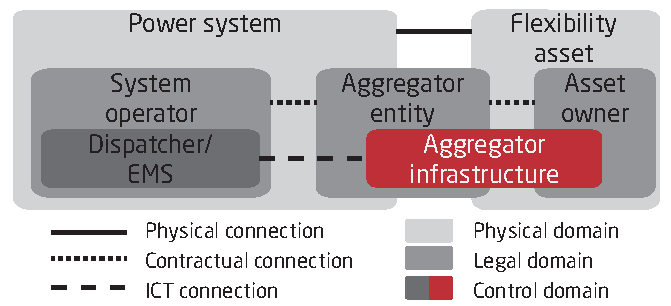
\includegraphics[width=1.0\columnwidth]{etfa2015/domains.eps}
\caption{The aggregator concept across domains.}
\label{fig:domains}
\vspace*{-5mm}
\end{figure}
\subsection{Clarifying the Aggregator concept}\label{subsec:clarifying}
The term \emph{aggregation} has different relevant interpretations in business, information technology,  control, as well as in the physical power system domain. Our concept of aggregators is illustrated in Fig.~\ref{fig:domains}, defining aggregators as a business role, aggregator entity, as well as a technical aggregator infrastructure.

The physical domain addresses the electrical interactions between flexibility assets (also referred to as DER) and power system. Whereas aggregation with respect to physical topology is a common concept (e.g. microgrids, cells), in our understanding, aggregators are not bound to aggregation with respect to physical network topology. 
%The aggregator is only reflected in this level by the manipulation of the interaction between the flexibility assets and the power system.

In the legal and business domain, an aggregator entity is an intermediary, maintaining contractual relations with flexibility asset owners and system operators (as receivers of flexibility services). The aggregator entity assumes legal responsibility for the delivery of a contracted service. The aggregator role may be filled by new independent market actors or be part of existing actors, such as utilities or balance responsible parties.

In the control domain, the aggregator infrastructure coordinates the behavior of flexibility assets. The control domain requirements are formulated as \emph{flexibility services} to system operators and \emph{asset management services} towards asset owners. Tracing these requirements for architectural validation and performance validation in the aggregator infrastructure is the focus of this paper.

The proposed aggregator concept is implementation agnostic and focused on formulation of functional requirements.

\subsection{The aggregator concept in technical literature}
There is no unanimous definition in literature of what could be considered standard functionality of an aggregator. This is reflected by the wide variety of aggregator designs\fcite{kok2005powermatcher,han2010development,sortomme2011optimal,costanzo2013coordination}, which differ in capabilities and purpose, and which use different (often implicit) criteria for classification.

Aggregators are commonly classified by control scheme into autonomous, indirect, transactional and direct control \fcite{Kosek}. Another classification emphasizes the commercial or technical focus of aggregators, referring to \emph{commercial} and \emph{technical} virtual power plants (CVPP and TVPP) \fcite{fenix2009}; however, as both types require business and technical functionality, the CVPP/TVPP distinction expresses a difference in degree and is not categorical. An advanced aggregator realizing the full functionality spectrum as \emph{Dynamic VPP} (DVPP) has been formulated in other work\fcite{niesse2014conjoint}. 
The proposed concept of aggregation encompasses all of the above but focuses on functional requirements for service provision, not business logic.

\subsection{Aggregator Business Harmonization and Standardization}
Whereas aggregator functionality is becoming a shared concept, there are still many models describing a) which stakeholders may benefit from the flexibility service, b) the form of the flexibility service, c) which stakeholders (are allowed to) perform aggregation and who should receive compensation \fcite{eurel-aggr} and d) how to harmonize the interaction between aggregators and aggregated units.

With respect to a), market models are being revised and new service models introduced to assign a value to flexibility (either directly to system operators as ancillary service, or as enhancement of flexibility of existing portfolios). The form of the service, b), is often formulated as an abstract flexibility service, a trade-off between both grid needs and generalized resource characteristics. Regarding d), many aggregators use proprietary communication, loosely based on standards (e.g. IEC61850 or IEC 60870-5-104; increasingly also OPC-UA); harmonization efforts in Europe continue to be addressed in the Smart Grid Coordination Group (SGCG) under EU Mandate M/490. A successful interoperability effort in this domain is the OpenADR standard published also as IEC PAS 62746.10-1. Meanwhile the IEC TR 62357 \emph{Reference Architecture to Smart Grid Information Exchange} is under revision. The reference architecture presented here focuses, within the Smart Grid Architecture Model\fcite{SGAM}, on functional interoperability for aggregators (field to operation zones; DER and customer domains) supporting interactions with System Operators, market actors, and devices at process level.

%\noindent\rule{4cm}{0.4pt}\\
%\textcolor{red}{(the follwoing defintioins belong into this section)}\\
%DEFINITION\\
%LEGAL\\
%Aggregator Role $\surd$\\
%Flexibility Asset Owner Role $\surd$\\
%SOFTWARE DOMAIN\\
%Virtual Nodes  (agents, processes) $\surd$ \\
%aggregator-side $\surd$ \\
%asset-side $\surd$ \\
%PHYSICAL DOMAIN \\
%Aggregator Site\\
%Flexibility Asset $\surd$ \\
%Device Interface $\surd$ \\ 

%#############################################
\section{The Need for an Aggregator Reference Architecture}
\label{sec:requirements}
%The power system is experiencing a paradigm shift. 
Existing concepts and methods for benchmarking and generator validation/certification cannot readily be translated from the (bulk) generator based paradigm to the distributed paradigm of aggregators and flexibility services. Historically, ancillary services have been defined using a physical understanding of generator capabilities. This definition is moving towards technology-agnostic service models.
Service verification has been done through on-site measurements, which is infeasible with thousands of units participating in service provision.  

The definition of a reference architecture for aggregators addresses these three issues, and enables benchmarking of aggregator architectures.
A reference architecture ``captures the essence of existing architectures, and the vision of the future needs and evolution to provide guidance to assist in developing new system architectures.''\fcite{cloutier2010concept}. It should provide: 
\begin{itemize}
\item a common lexicon and taxonomy,
\item modularization and the complementary context, and
\item a common (architectural) vision.
\end{itemize} 

%1) new industry -> benchmark, kpis certification is needed, since they cannot be translated from the old industry 
%
%2) service verification is different -> traditionally expensive measuring equipment. new method is needed for new architecture
%
%3) technology agnostic service models, rather than technology based services. Need an architecture to standardize context
%The common lexicon and taxonomy allows for precise discussion and a common understanding of what an aggregator is and can do. The establishment of these two concepts is started in Section~\ref{subsec:clarifying}, where the context of the aggregator is also discussed.% and further refined throughout the paper. 
Various types of aggregator implementation exist, realizing different design ideas for different sets of requirements. These requirements -- and consequently the designs derived from them -- are unlikely to converge towards a single solution because of the tradeoffs involved, e.g. scalability and complexity. A common lexicon and taxonomy is a minimal precondition for aggregator comparison.
If a reference architecture is to be used to describe many of these different designs, it must be highly modular. In practice, the \emph{general} functionality of an aggregator must be broken down into small enough functions in order for these functions to be usable as building blocks for the reconstruction of the \emph{particular} functionality of a given implementation. 
The functions are arranged in a reference architecture such that metrics can be assigned to individual functions. In this way, the reference architecture can be used for validation of the aggregator. Our architectural vision accounts for the need for verifying distributed flexibility services.

%Implementability (discuss what that means in this context?)

%The methodology for the analysis is the following:
%\begin{itemize}
%	\item We have analyzed different aggregator architectures from the literature, as well as the experience gained through the practical implementation of an aggregator in our laboratory, and extracted the essential functionalities necessary for the working of the aggregator. These functionalities are independent from aggregator/control architecture.
%	\item We analyze the functions and their relationships, as well as the level of complexity we can foresee.
%	\item Synthetize the results into a reference architecture. 
%	\item Validate by mapping different architectures into the framework.
%\end{itemize}


%This is still part state of the art, so this and the previous section together shouldn't be too long)
%\begin{itemize}
%\item \textit{The method}
%\item Why would somebody want to evaluate aggregator performance?
%\item Which methods/approaches for performance evaluation exist or are being discussed?
%\item What is missing? (A reference architecture of course, but why?)
%\end{itemize}

%#############################################
\section{Functional decomposition}
\label{sec:funcdec}
An aggregator is a complex system of interacting functions. In the following definitions, we abstract from implementation details, e.g. centralized vs. distributed systems, and focus purely on the purpose of the functions. 

% EXTERNAL INTERFACES
%\subsection{Service Interface}
\textbf{A. Service Interface}
The service interface translates the contractual agreements between the aggregator and its clients into a service model containing quantifiable and measurable service requirements and a set of performance criteria. This service model is then used to map incoming service requests to control domain signals such as control variables, constraints or control parameters.


% Monitoring & Supervision modules
%\subsection{Performance Monitoring}
\textbf{B. Performance Monitoring}
The performance monitoring function collects data from which the behaviour of individual clients can be derived. The data is analyzed to determine the performance of a client, and its compliance with the contracted flexibility service. This analysis may be internal to the performance monitoring function, or it may simply serve as a data gatherer for an external entity.


%\subsection{Supervision and Resource Handling}
\textbf{C. Supervision and Resource Handling}
The aggregator must maintain an overview of available client resources and their status. By comparing the communication status and monitored performance of individual clients to the control signals sent by the aggregator, the supervision function determines whether clients perform according to their contract. It may temporarily or permanently exclude non-compliant clients from the pool of available resources.


%\subsection{Operator Interface}
\textbf{D. Operator Interface}
Although the power system is moving towards automated solutions, decision-making on critical issues is the responsibility of human operators. The aggregator architecture must support decision-making by presenting operators with the necessary information, and facilitating operator input and intervention.  %\textcolor{red}{(Incomplete/rewrite!)}


% Control-related
%\subsection{Control}
\textbf{E. Control}
The control function is in charge of generating the appropriate control domain signals for the portfolio. Depending on the control architecture, the control logic may be distributed between physical entities. The concept of a control domain signal covers several kinds of signals, including, but not limited to control inputs to DERs, coordination messages for distributed control and reference signals for hierarchical controllers.


%\subsection{Flexibility Monitoring}
\textbf{F. Flexibility Monitoring}
In operation, the aggregator must assess the future flexibility of its portfolio in real time; this includes individual DER flexibility as well as the aggregated flexibility of the portfolio. The flexibility assessment can either be based on direct feedback from the DERs or entirely on estimation models (possibly stochastic) if direct feedback is not available.

% Communication
%\subsection{Aggregator-internal communication}
\textbf{G. Aggregator-internal communication}
Except for very few special cases, aggregation will almost always be implemented as a distributed computing system. In its basic form, such a system would consist of one aggregator and a number of clients. This may be extended by stacking multiple levels of aggregation etc. The internal communication function exchanges information between aggregator and clients.


%\subsection{Client management}
\textbf{H. Client management}
The client management function actively or passively tracks the availability of clients. It may also provide a mechanism for the dynamic addition and removal of clients, such as a discovery service, and maintain a protocol for temporarily disabling otherwise available resources. It contributes to resilience and graceful degradation of the portfolio.



%\subsection{External Information Services}
\textbf{I. External Information Services}
To be able to act optimally with respect to both control of its portfolio and trade of electricity in forward markets, aggregators will likely have to rely on different types of information services. Such services include different types of forecasts and measurements in real time and may be provided by either internal processes or by a 3rd party. 


%\subsection{Asset interface}
\textbf{J. Asset interface}
Most aggregators in a Smart Grid context will be used to harvest flexibility from existing energy resources. In most cases communication between aggregator and resource will use a fieldbus-style interface not designed for wide-area communication. The purpose of the asset interface is to maintain communication with a physical unit under aggregator control and provide abstraction from interface details.


% the odd one
%\subsection{Information Exchange}
\textbf{K. Information Exchange}
Virtually any modular software framework contains a facility for information exchange between its components and storage of the overall system state: static data, dynamic data or both. A knowledge exchange may take many different forms, from a collection of object references towards a central or distributed database. 


%#############################################
\section{The Reference Architecture} 
\label{sec:refarch}
% === This is where we collect the knowledge collected in the previous section into the actual architecture and discuss it and its building blocks. (Introduce complexity levels) ===

We have now established a set of functions to serve as building blocks for a reference architecture, but without concern for the relations between these blocks. Next, these relations will be examined; in other words: how could a practical aggregator infrastructure be composed from these function blocks?

\subsection{Function blocks and knowledge exchange diagram}

% === Explain what the function blocks symbolize - and how the location in the function block diagram does not say anything about whether a block exists on the aggregator side, the client side or both. ===

The functions in section \ref{sec:funcdec} generally belong to one of the following categories:
\begin{itemize}
\item functions dedicated to communication between physically separate parts of the aggregator infrastructure or communication with 3rd party entities, i.e. enablers of the distributed nature of the system.
\item functions which perform decisions with regards to flexibility asset behavior and portfolio composition.
\item functions which interpret information and support the decision making functions. 
\end{itemize}
These categories represent requirements for different architectural paradigms: Communication functions are layered or hierarchical, and, in the case of communication between aggregator and client, require an identically layered counterpart at the opposite end. The decision making and interpreter functions on the other hand require many hierarchical and non-hierarchical consumer-producer relations. % The interpreter functions generally exist in direct relationship with the decision making functions. %The knowledge exchange function, storing the different elements of system state, provides a link between these two worlds.  
Figure~\ref{fig:functiondiagram} shows an overview of the relationships between functions according to the above concept.

\begin{figure}[htb]
\centering
\includegraphics[width=1.0\columnwidth]{"etfa2015/diag_simple"}
\caption{Each function outputs distinct kinds of data which are used by the other functions in different ways according to the aggregator implementation.}
\label{fig:functiondiagram}
\end{figure}

\subsection{Principles of distribution of functions}

While figure \ref{fig:functiondiagram} depicts the relationship between aggregator functions, it does not include information about the physical distribution of these functions between the asset side and the operator side of the aggregator infrastructure. This distribution is highly specific to the individual design and e.g. its degree of centralization (see section \ref{sec:applic}).

In an actual implementation, several of these functions require corresponding instances on each side, effectively forming a communication stack. 

The functions exhibiting these properties are:
\begin{itemize}
\item the internal aggregator communication function which provides the link between the two substacks. In many cases, this function will make use of a full OSI-layered stack in which the internal aggregator communication function provides the application layer,
\item the client management function, implementing management protocols which would typically require a corresponding instance on the client side, and
\item the knowledge exchange function which exchanges information with its client side counterpart independent of client management mechanisms.
\end{itemize}

All other functions, with the exception of the asset interface, may appear either on the operator side, on the asset side, or shared between both sides, depending on the implementation.

%#############################################
\section{Case studies} 
\label{sec:applic}

A number of existing aggregator designs -- commercial as well as academic -- have been mapped to the model in order to test its viability. Two cases with different design philosophies are presented here in order to illustrate the distribution of functionality between the operator and the asset side, and the information flow between the functions:
\begin{itemize}
	\item \emph{Power Hub} is an aggregator developed by Dong Energy in Denmark. It is used to control distributed generation and load in order to sell flexibility services to the ancillary power market (Figure~\ref{fig:powerhub}).
\item \emph{Open Energi} is a British company selling flexible consumption from industrial loads as an ancillary service. The aggregator functions are distributed between an operator node at a control center and asset nodes on custom hardware deployed at customer sites (Figure~\ref{fig:openenergi}).
\end{itemize}

The most significant difference between the two designs is the degree of autonomy of the asset node. The Power Hub concept is based on a centralized design which mainly uses the asset node as a communication gateway and places flexibility monitoring and control at the central operator site. This is also where external information such as market data is available through the information services function.
The Open Energi controller acts on quantities measurable at the asset site and does not require external information; this allows control and flexibility monitoring to be placed at the asset node, leaving only supervisory functions at the operator site.

Both designs can be split into functions according to the subdivision proposed in section \ref{sec:funcdec}.

\begin{figure}[htb]
\centering
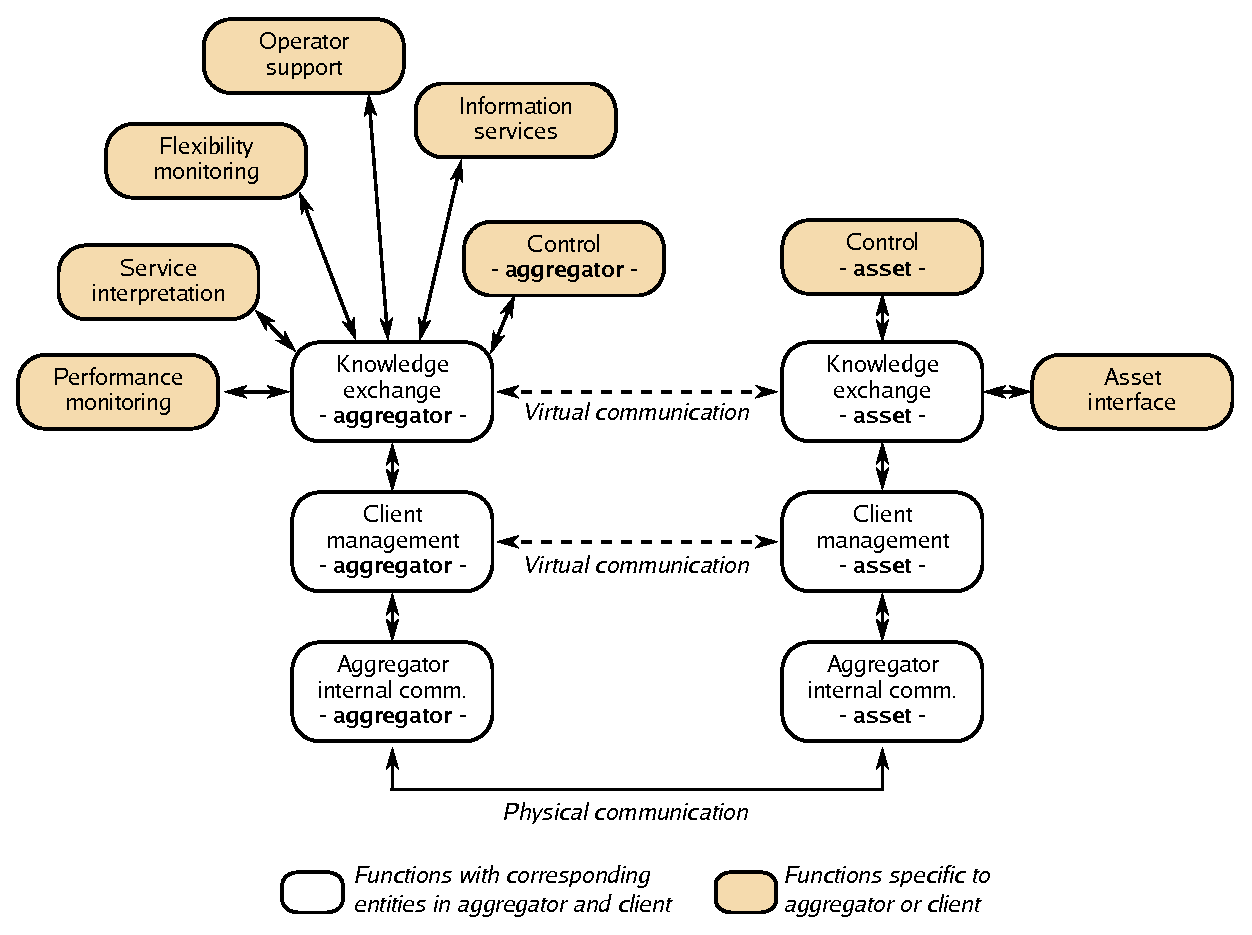
\includegraphics[width=0.65\columnwidth]{etfa2015/stackdrawing_powerhub.eps}
\caption{Distribution of functions for the Power Hub aggregator}
\label{fig:powerhub}
\vspace*{-5mm}
\end{figure}
\begin{figure}[htb]
\centering
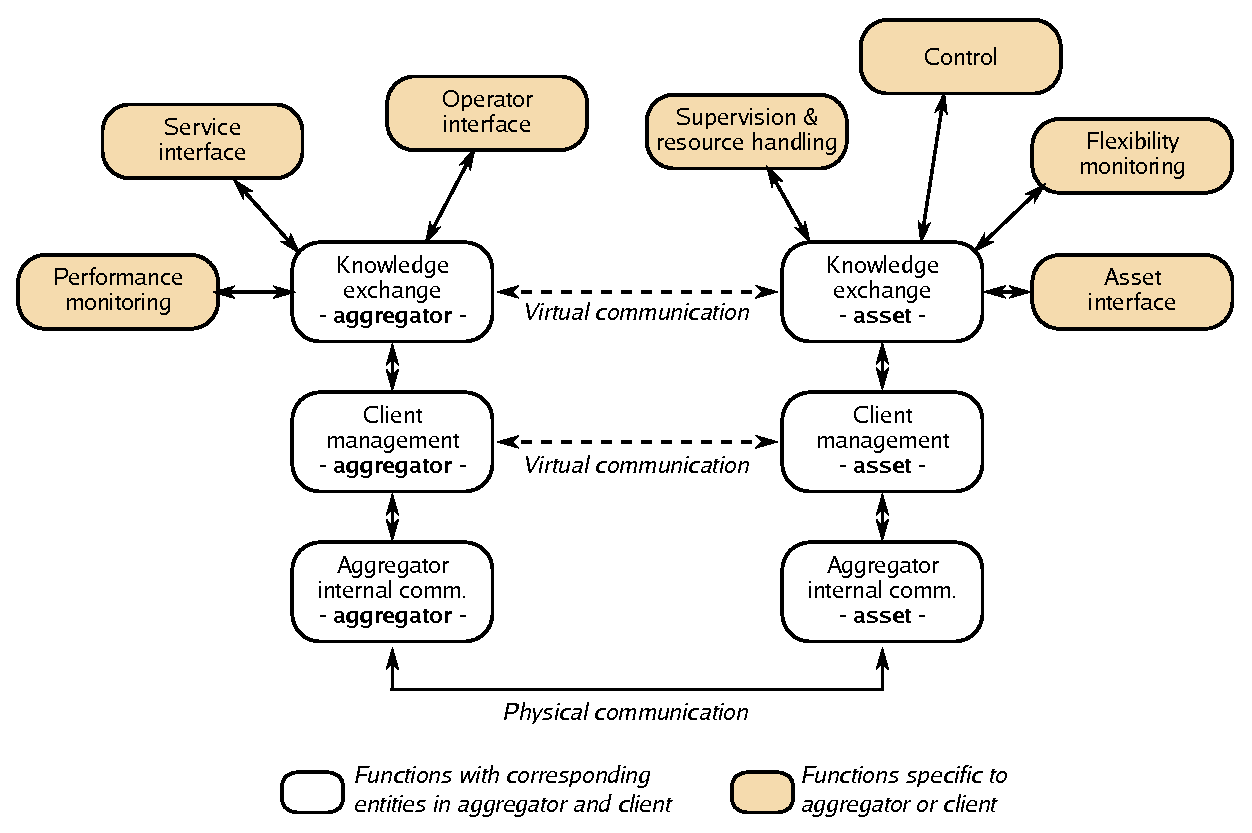
\includegraphics[width=0.65\columnwidth]{etfa2015/stackdrawing_openenergi.eps}
\caption{Distribution of functions for the Open Energi aggregator}
\label{fig:openenergi}
\vspace*{-5mm}
\end{figure}



%#############################################
\section{Conclusion and further work}
\label{sec:etfa2015:conclusion}
A reference architecture for the validation and comparison of aggregators has been presented. While the general framework has been established and successful mapping tests to a number of real-world aggregator designs have been performed, many details are still work in progress.
The next steps towards completion will be the development of performance indicators for the individual functions and the establishment of a process for aggregator comparison and performance validation.

%Review 1: As the goal of the paper is to develop a reference archcture, please elaborate on reference architectures in general and on the SGAM in particular.

%
%Review 2: The WIP-paper presents a high-level reference archcture for the validation and comparison of aggregators for power system services from distributed energy resources. Based on a functional decomposition of practical implementations a reference architecture is developed. It is validated against two practical implementations (power hub and open energi). 
%
%The value of a reference archcture for the crucial role of aggregators such as this is obvious but the developed architecture needs to be validated with more practical examples. How and if this architecture may be used performance evaluation, comparison or even optimization of aggregators remains to be proven. But the paper definitely meets the requirements of a WIP contribution.

%Review 3:	The concept of the reference archcture is nicely introduced and explained. Since it is a work in progress paper a more detailed presentation of future work would be appreciated.

%#############################################
\section*{Acknowledgment}
Parts of this work are supported by the Programme for Energy Technology Development and Demonstration (EUDP) and Innovation Fund Denmark through the iPower project.


\chapter{Procedure for Validation of Aggregators Providing Demand Response}\label{app:pscc2016}

\textbf{Authors:}\\
Daniel Esteban Morales Bondy\\
Oliver Gehrke\\
Anders Thavlov\\
Kai Heussen\\
Anna M. Kosek\\
Henrik W. Bindner

\noindent
\textbf{To be presented at:}\\
Power Systems Computational Conference, 2016 \\
Genoa, Italy


\noindent
\textbf{Abstract:}\\
As aggregators become viable sources of ancillary services, they will be required to undergo a validation process similar to the prequalification process of traditional generators. Since aggregators are fundamentally different from traditional generators, a new test method must be designed for the aggregator validation. This work proposes a method for designing the tests necessary for the validation process. The method is exemplified with a study case and results are presented.
\section{Introduction}
As renewable energy generation increasingly replaces conventional power plants, power system operators are looking for alternative sources for the ancillary services which were traditionally provided by these plants. It is expected that some ancillary services can be procured from distributed consumption and production units by making use of their unused operational flexibility. In order to provide coordinated services, such as demand response, from a large number of such distributed energy resources (DERs), a new actor is appearing in the power system: the aggregator \fcite{gkatzikis2013a}.% \hl{I was wondering whether we should clarify which type of aggregator we're talking about here, to make it harder for nitpicking reviewers.}\textcolor{red}{You mean commercial VPP vs Technical VPP?}

Conventional sources for ancillary services must be %certified/
validated before being able to offer control reserves in an ancillary services market \fcite{energinettender}. It is expected that aggregators will be required to undergo a similar validation process to ensure the integrity of the provided service with respect to predefined requirements.

The cost of establishing an aggregator is driven partly by the cost of establishing the associated control and communication infrastructure. The communication infrastructure requirements and installation effort are strongly dependent on the chosen aggregator architecture \fcite{kosek2013overview}. The achievable performance with a given concept also depends on this architecture. %\hl{Do we have a reference for that statement?}\textcolor{red}{I don't think so, but isn't logical? Direct and indirect control will have very different infrastructure implementations... I think rather I'm not clear in what I'm trying to express} 
Therefore new methods and tools are needed to validate an aggregator architecture, in terms of capability to deliver the desired services. Such an assessment of an aggregator can be relevant before investments into a particular infrastructure are made. The methods may also be incorporated into a future aggregator validation process.

The purpose of this paper is to derive the testing specification for an aggregator from its contracted service requirements. Specifically, we constrain the analysis to active power services such as frequency containment and frequency restoration reserves \fcite{entso1operational} for transmission systems and congestion management for distribution systems. %of the interaction between the systems interacting directly or indirectly with the aggregator. \textcolor{red}{The word interaction is used too much here, how do I fix this?}\hl{I'm not sure if I know what you want to say. "testing of the interaction between the systems interacting with the aggregator" - what interacts with what here? My best bet right now is "The purpose of this paper is to describe the alignment of service requirements with the testing specification of the aggregator, including the interaction between its subsystems." Is that what you meant?}

\section{Conventional resource validation and aggregator differences}
%\hl{ We explain why system operators want resources to be validated (WHY?) }
Ancillary services are essential for the reliability of the power system. Because these services play such an important role in the safe operation of the system, it is essential that the units or entities providing a service perform according to the requirements set by the Transmission System Operator (TSO). These requirements and processes are typically specific to a particular TSO and influenced by national regulations, interconnection grid codes etc. Two examples are regulations established by Energinet.dk and PJM.
\subsection{Current requirements for prequalification}\label{sec:PSSCCconventionalvalidation}
In Denmark, Energinet.dk, the danish TSO, ensures the appropriate service performance by requiring all units participating in the ancillary service markets to provide a documentation of their capabilities and go through an approval process \cite{energinet2012ancillary}. This approval process consists of a test conducted at least three weeks prior to the service delivery date. The tests for Frequency Containment Reserve (FCR) generally involves the injection of a setpoint step into the plant's governor and the measurement of the response. The test for Automatic Frequency Restoration Reserve (A-FRR) involves the tracking of a reference signal from Energinet.dk. Currently, this procedures are not formally described.
Demand resources are expected to provide a substantial amount of the ancillary services for the Danish grid in the future. Since distribution system services are not widespread yet, the concept of unit certification is non-existent at the distribution level. 

%\hl{Here we explain the current method for resource validation. (HOW?)}
%\hl{There is abig jump form Demnark to US, maybe we can sat that Denmark has not such regulations and US is more advanced in the process...}
While Denmark is starting to open up to new sources of ancillary services and standardise its test procedures, PJM (a regional transmission operator in the United States) has a standardised prequalification procedure for regulating resources\footnote{Regulation in the US corresponds roughly to the FRR of ENTSO-E.}, which consists of three consecutive area regulation tests, where PJM Performance Compliance scores indicate how well the resource follows a simulated regulation signal. A single test lasts for 40 minutes and in order to pass it the unit must score at least 75\% in three consecutive tests  \cite{pjm2015balance}. While this rule includes services provided by multiple generators at a single site, operators of demand resources are not required to be certified but must complete an initial training module on the requirements and business rules of the Regulation and Synchronized Reserve markets \cite{pjm2015certification}. Currently demand resources are only allowed to form 25\% of the total regulation \cite{pjm2015ancillary} in PJM, and therefore their certification process is still not a large concern. 

In both systems the validation tests have two goals: to ensure the communication with the units works correctly, and to validate the known performance model of the generators. Thus, a change of configuration in the setup requires a new certification of the generator. Also, a dedicated communication and measurement infrastructure between system operator and aggregator is required. The measurements must have high sampling frequency, e.g. better than 10 mHz, and high precision, e.g. sensitive to frequency deviations of $\pm$ 10 mHz. Measurement equipment that respect these requirements is expensive.
%\hl{We show in which way the current method is not applicable to aggregators and other distributed / multi-resource service providers, and conclude that an alternative method is needed (WHAT?, problem statement)}
\subsection{Problems applying current validation methods to aggregators}
The tests outlined above are specific to each system operator, but follow similar paradigms. 
The conventional test processes cannot be directly applied to portfolios of aggregated resources, mainly because a common assumption in the process is that the service delivery is performed by a single or small number of units. This allows inference of the unit's ramp capabilities through a response test, based on a known model. Also, a limited amount of precise and expensive measurement equipment needs to be installed.

An aggregator and the portfolio of units under its control behave fundamentally different from large generation units:
\begin{enumerate}
\item Individual generator units are well understood and models describing their static and dynamic properties are readily available. This is not the case for portfolios of aggregated units which are typically heterogeneous and can only be modelled through their statistical properties. This is aggravated by the fact that unit portfolios may be dynamically reconfigured during operation.
\item There is no direct equivalent to a single point of measurement: An aggregator's portfolio may consist of geographically dispersed units. Their aggregate power profile does not correspond to a measurement at any single point of the grid. Coupled to this, it is economically infeasible to install the required expensive measurement equipment at each DER.
\item Aggregators, by definition, operate a distributed system (both in control and geographical terms) in which each unit has its own response properties and requirements. This leads to an aggregated response that behaves differently from that of conventional generators.
\item Reliability concepts for distributed systems are different; specifically, the failure modes are not the same. If a component of a monolithic generator unit fails, the whole unit may have to shut down. The failure of a single unit in an aggregator portfolio will often have a minor or negligible impact on the overall performance. In a large portfolio it will usually be possible to recruit an equivalent replacement unit providing the same services as the failed one.
%\item There are many different ICT and control architectures for aggregators, and interoperability standards must be used for the internal workings of the aggregator. \hl{and whats the point?}
%\item The primary purpose of units composing an aggregator is to serve a specific energy-dependent need of the unit owner, not to provide the flexibility service, hence not all units in an aggregator portfolio may always be available.\hl{This is a property of e.g. demand response, not of aggregation. It applies to a single DR unit as well. I'd skip this argument.}
\end{enumerate}

For the above reasons, the same validation and service requirements cannot be applied to aggregators. This paper focuses on reinterpreting the validation tests to aggregators by adapting concepts from statistical testing to the power systems domain. 



%is not as straightforward for aggregated systems due to their geographical distribution, dynamic nature, complex ownership structure, and possible difference between the service requirements of individual units and the aggregate as a whole.
%The service requirements may also differ between demand response and traditional ancillary services, which leads to different validation requirements.\textcolor{red}{better?}

\section{Test requirements and proposed test  method}\label{sec:metrics}
%\hl{- What alternative method do we propose?}

The objective of the current tests is to validate the parameters of a well understood model of generation units. For the reasons given above, the new tests need to identify an empirical behavior model of an uncertain and diverse entity: the aggregator control architecture and unit portfolio. 

%This means that there is no single standard test, but 
A method is required to design the tests that will allow the system operators to understand and predict the performance of a specific aggregator under a given set of operation conditions (Fig.~\ref{fig:framework}). In this section we explain the underlying assumptions regarding the operating environment, the service requirement metrics used to measure the aggregator performance, and the proposed test design method.
%Getting an empirical model of an unknown entity rather than a mathematical model of a known entity. System identification approach.

\begin{figure}[!t]
\centering
\includegraphics[width=1.7in]{pscc2016/validation.eps}
\caption{Schematic process for aggregator validation. The focus of this paper is on the relationship between the service requirements and the aggregator tests.}
\label{fig:framework}
\end{figure}

%Here the following three topics must be discussed:
%\begin{itemize}
%\item Boundary conditions (grid, DER)
%\item Fault scenarios
%\item Operation spectrum (what is the possibility/range of the input data?)
%\item Experimental design
%\end{itemize}

%The experiments should be able to measure response/states that can't be measured safely/easily under deployment.

%The tests must have a well defined input and output.

\subsection{Test environment assumptions}
The objective of the aggregator validation tests is to subject the aggregator to disturbances such that it can be verified that the aggregator is capable of respecting the service requirements under a set of expected operation scenarios. While the design of these operating scenarios is outside the scope of this paper, some overall assumptions can be made.

A great variety of aggregator architectures has been proposed and implemented; differences between them are linked to specific business cases, local regulations, grid codes etc. Implementation details such as algorithms for portfolio composition, resource prediction or trading, constitute key intellectual property of commercially operating aggregators and disclosure of these business secrets will be unacceptable in many cases. For this reason, a general test design must start from the assumption that the aggregator and its infrastructure are to be treated as a black box, in the sense that only the aggregator inputs and outputs are known but the details of the internal control architecture are unknown. 

While a few tests are enough to ensure compliance of traditional generators, the stochastic nature of aggregators requires the tests to be repeated a sufficient amount of times in order to capture the variance of the stochastic process that influences the aggregator performance. These stochastic processes, e.g. weather conditions or user behaviour, form the disturbances in the test. It is usually infeasible to subject a deployed and operational aggregator to a high number of tests, it is expected that aggregator validation must include simulation. In this way, the aggregator will be subjected to situations that are reproducible. It is assumed that such a simulation framework is detailed enough in terms of power system models, DER models and information and communication technology (ICT) systems in order for the simulation results to reflect the real performance of a deployed aggregator with sufficient precision.

The tests are composed of a set of operational scenarios and service requirements (Fig.~\ref{fig:framework}) wherein the operational scenarios define the statistical distribution of the test disturbances and the service requirements define the expected behavior of the aggregator. The mode of interaction between the test cases and the aggregator is defined in a test setup (Fig.~\ref{fig:test_setup}), where the disturbances (test inputs) defined in the operational scenarios affect the aggregator interaction with the DERs and the power grid. The aggregator has two interfaces:
\begin{itemize}
\item Input: Measurements or reference signals received from the system operators.
\item Output: Control domain signals and measurements exchanged between the aggregator and the units in its portfolio.
\end{itemize}

The operational scenarios are not designed to cover aggregator operation under exceptional system conditions. This means that the aggregator will not be held accountable for non-delivery in cases where the cause is outside of the aggregator's influence, e.g. in the case of grid faults. If communication between the aggregator and the controlled units, or internally within the aggregator architecture, occurs over public telecommunication networks, the robustness to network outages must be tested, for example by simulating disturbances and delays.

Finally, the flexibility which the aggregator can offer is bounded by the contractual requirements between the aggregator and its clients.

\begin{figure}[!t]
\centering
\includegraphics[width=\columnwidth]{pscc2016/test_setup.eps}
\caption{Schematic test setup where the test subject, the aggregator, is treated as a black box.}
\label{fig:test_setup}
\end{figure}

\subsection{Test service requirement metrics}\label{sec:servreqmet}

In order to measure how the disturbances affect service delivery, a set of service performance metrics must be established. The main purpose of the current tests is to verify communication, responsiveness to frequency changes and tracking of a reference or AGC\footnote{Automatic Generation Control, see e.g.\cite{entso1operational}.} signal. Coupling this with the performance requirements defined by the TSOs\cite{energinettender,ipower2013development}, the expected behavior of the considered services was analyzed (Table~\ref{tab:servmet}), and a set of requirement metrics were defined:
\begin{itemize}
\item Time responsiveness, i.e. how fast can the service be delivered from the moment the reference or measurement signal changes.
\item Grid responsiveness, i.e. how well can the aggregator follow changes in the grid state (marked with $\star$ where relevant on Tab.~\ref{tab:servmet}).
\item Response accuracy, i.e. how good is the aggregator in providing the full volume that is requested.
\end{itemize}


\begin{table}[!t]%% increase table row spacing, adjust to taste
\renewcommand{\arraystretch}{1.3}
% if using array.sty, it might be a good idea to tweak the value of
% \extrarowheight as needed to properly center the text within the cells
\caption{System services and their behavior}
\label{tab:servmet}
\centering
% Some packages, such as MDW tools, offer better commands for making tables
% than the plain LaTeX2e tabular which is used here.
\begin{tabularx}{\columnwidth}{p{1.0cm} X X}
\toprule
System Operator& Service name & Service behavior\\
\midrule
TSO & Frequency containment reserve (FCR) & autonomous response to frequency deviations ($\star$) \\
TSO & Frequency restoration reserve (FRR) & tracking of the AGC-signal\\
DSO & Congestion management         & reference tracking \\
    &                               & respecting a maximum feeder/transformer limit ($\star$) \\
    &                               & demand response \\
    &                               & grid state responsiveness ($\star$)\\
\bottomrule
\end{tabularx}
\end{table}

These three metrics will conform the measure with which an aggregator will be deemed to perform according to service requirements, and the tests must excite the aggregator such that it is possible to determine through the value of these metrics the performance of the aggregator. It must be pointed out that the grid responsiveness metric is only applicable to the evaluation of aggregators providing services that rely on direct measurement of the grid, e.g. FCR.

It is assumed that the validation tests will be carried out in simulation so that the tests can capture the stochastic nature of the disturbances. Therefore, when system operators define the acceptable values of the service requirement metrics, the values should have a statistical component. An example could be that the time responsiveness of a service provision should in average of 5 seconds, with a variance of $\pm$ 1 second. The actual indices used for the proposed metrics are discussed in Sec.\ref{sec:evaluation}.

\subsection{Aligning service requirements and tests}\label{sec:alignment}
In order to align the service requirements and the test design, we propose the following steps:
\begin{enumerate}
	\item The aggregator informs of the general composition of its portfolio, as well as the service it wants to be validated for.
	\item The tester identifies the appropriate service requirements for the service to be tested for.
	\item The tester identifies the expected normal operation of the aggregator.
	\item The tester defines the operation scenarios that the aggregator is expected to perform under. The scenarios must define the statistical properties, e.g. mean and variance, for the stochastic disturbances affecting the aggregator performance.
	\item The tests are carried out on the aggregator.
	\item The aggregator performance is evaluated.
\end{enumerate}

From the services analysed in this work, we divide the tests into two categories depending on their excitation signal:
\begin{itemize}
\item step response (like those for FCR),
\item continuous reference tracking (like those for FRR).
\end{itemize}

The validation tests will use one of these excitation signals under a different set of circumstances defined in the operation scenarios. The same excitation signal will be applied to the aggregator a sufficient amount of times to ensure that the mean and variance of the performance metrics give a realistic impression of the aggregator performance under deployment.%Thus, we formulate the following heuristic for the alignment of service requirements and tests: if a service
%The tests will evaluate the sensitivity of the aggregator to changes in the portfolio, and issues with the communication.

A drawback of this method, in comparison with the traditional test method, is that the overall validation method rely on the accuracy of the simulation models. The test architecture that validates the aggregators itself would need to be validated. This applies to the communication systems, the grid models and the DER models.

%\hl{The test procedure should be described. 2 diagrams are needed: 1st. shows the aggregator under normal operation (physical connection and the ICT connection), with relevant inputs and outputs of the aggregator. 2nd is the test process, where at each stage inputs are added/modified.}

% At the same time, based upon these two inputs, the overall service delivery is verified and evaluated, which is reflected in the bottom box of Figure~\ref{fig:framework}. \hl{Generally, I think we're still talking too much about the overall process and not about what the paper claims it's focusing on ("[...] the alignment of service requirements with the testing [...]"). On the latter we're not specific enough wrt what kind of result the reader can expect.}

%An aggregator infrastructure and control process is usually complex and therefore interactions of an aggregator may be tested separately. Depending on the metrics by which the relations are measured (Table~\ref{tab:metrics}), it is possible to test certain components through simulation or co-simulation, while other interactions require hardware-in-the-loop tests. This paper will propose a method for identifying the relationships between metric types and the tests necessary  for validating the measured function. The method will then be applied to several existing aggregator architectures as a proof of concept.

\subsection{Test evaluation}\label{sec:evaluation}
The service requirement metrics (Sec.~\ref{sec:servreqmet}) define the measure upon which the aggregator is evaluated. Different options exist that can be used to measure these metrics. One option is the aggregator performance index\cite{bondy2014performance}, which measures the error in service delivery for the services delivered to the system operators and the serviced delivered to the owners of the DERs. This metric captures both time responsiveness and response accuracy into a single value. A large set of performance indices exist within the field of control performance assessment, these can be utilised for the proposed validation method\cite{jelali2006overview}.

Given the stochastic nature of the tests, the indices will also be stochastic. The value of the performance indices is estimated at each iteration of the test, which means that the final value of the performance index reflects the stochasticity of the disturbances. For example, if the disturbances defined in the operation scenarios are Gaussian, the performance index will also have a mean and variance. These values need to be compared to those values defined in the service requirements. It will be the choice of the system operators what the service requirements should be, taking into consideration their risk adversity. Requiring a small variance on the performance indices minimizes the risk of not getting a full service delivery, but might also lead to more expensive services.


%\input{content/assumptions.tex}
\section{Case Study of the Validation Procedure }\label{sec:casestudy}

In this section we apply the concepts outlined in Sec.~\ref{sec:metrics} on a simplified example of the validation procedure on an aggregator architecture similar to the one presented in \cite{thavlov2013aggregation}. While the design of these operating scenarios is outside the scope of this paper, some overall assumptions have been made. The sample aggregator name is  DTU-FlexServices, and it wants to sell ancillary services to the TSO called RisøGrid. The validation tests are carried out by the independent company AggTesters. The rest of this section presents the reference scenario, the example of the aggregator test and the evaluation process. 

\subsection{Aggregator Framework \& Portfolio}
The objective of the DTU-FlexServices is to allocate a given amount of power, provided as a setpoint by the TSO, over a controllable portfolio of 100 resistive heating systems, each providing space heating to a detached household. The objective is subject to constraints on nominal power of the heating systems and indoor comfort, which is implemented as a tolerable band in which the temperature is allowed to vary given by the interval $\left[T_{min},T_{max}\right]$. It is assumed that feedback on measured indoor temperature is available to the aggregator, such that the aggregator in real-time can assess the available capacity of the controlled heating system and ensure that indoor temperature constraints are not being violated during operation. Fig. \ref{fig:flow_diagram} presents the flow of data in the aggregator simulation framework. 
\begin{figure}[!t]
\centering
\includegraphics[width=\columnwidth]{graphics/pscc2016/flowchart.eps}
\caption{Flow diagram of the aggregator algorithm.}
\label{fig:flow_diagram}
\end{figure}
The aggregator uses a simple auto-regressive model with exogenous inputs (ARX) to assess the future available capacity of each individual households. The ARX model is given by,
\begin{equation}\label{eq:capacity}
  T_{i+1} - a\cdot T_i = b \cdot T_{a,i} + c \cdot \Phi_{s,i} + \boldsymbol{d}^T \boldsymbol{\Phi}_{h,i:i-\tau_{lag}}
\end{equation} 
where $T_i$ is the measured indoor temperature of the household at time step $i$, $T_a$ is the outdoor temperature, $\Phi_s$ is the solar irradiance and $\boldsymbol{\Phi}_{h,i:i-\tau_{lag}}$ is a vector with the most recent observed power consumptions, i.e. $\left[\Phi_{h,i},\Phi_{h,i-1} \cdots \Phi_{h,i-\tau_{lag}}\right]$. The lag parameter of the heat input, $\tau_{lag}\in\mathbb{N}_0$, is used to account for the potential time-lag that might exists between when heating is applied and when it is observed in the indoor temperature. $a$, $b$, $c\in\mathbb{R}$, and $\boldsymbol{d}\in\mathbb{R}^{\tau_{lag}+1}$ are the unknown parameters of the ARX model, which are found using prior data for power consumption of the heating system. For simplicity $\tau\equiv 0$ is assumed in the following. 

Each individual resistive heating system is assumed to be able to dispatch a continuous amount of power in the interval $\left[P_{min}, P_{max}\right]$, given by the nominal power of the heating system. Naturally, this is an approximation since resistive heating systems, in general, will only be able to dispatch power in discrete steps due the composition of resistive loads. However, considering a portfolio of many entities and following the law of large numbers, these discrete steps should level out and the assumption hold. 

To allocate the amount of power over the portfolio of resistive heating system, following unit commitment problem is formulated,
\begin{align}\label{eq:agg_dispatch}
  & \min\;\left|\; \sum_{j=1}^N \left(\Phi_{h,i,j}\right) - S_i \;\right|\; + \; \sum^{N}_{j=1}\Phi_{h,i,j}\mbox{W}\left(T_{i+1,j}\right)	\\[5mm]\nonumber
  & \mbox{s.t.} \quad P_{min,j} \leq \Phi_{h,i,j} \leq P_{max,j}  
\end{align}
where the decision variable  $\Phi_{h,i,j}\in\mathbb{R}$ is the amount of power being allocated to household $j$ at time step $i$, $N$ is the number of households in the portfolio, $S_i$ is the setpoint given to the aggregator and $\mbox{W}\left(T_{i+1,j}\right)$ is a weight function of the predicted indoor temperature found from Equation \eqref{eq:capacity}. The weight function should be constructed such that $\mbox{W}\left(\cdot\right)<-1$ for $T_{i+1,j} < T_{min}$, thus making the last term dominate the cost function and force the allocated power up for household $j$. Likewise, $\mbox{W}\left(\cdot\right)>1$ for $T_{i+1,j} > T_{max}$, thus forcing the power down. Following linear weight-function is proposed,
\begin{equation}\label{eq:weight_fct}
  \mbox{W}\left(T_{i+1,j}\right) = \frac{2\left(T_{i+1,j}-T_{min,j} \right)}{T_{max,j} - T_{min,j}}-1 
\end{equation}
The simulation model of the individual households is implemented as a stochastic linear state space model in discrete time, which is     given by
\begin{align}\label{eq:simulation_model}
  \boldsymbol{T}_{i+1} &= \boldsymbol{A}\boldsymbol{T}_i + \boldsymbol{B}\boldsymbol{U} + \boldsymbol{\sigma}_i \\\nonumber
  T_i &= \boldsymbol{C}\boldsymbol{T} + e_i
\end{align}
where $T_i\in\mathbb{R}$ is the locally measured indoor temperature which is assumed to be forwarded to the aggregator, $\boldsymbol{T}_i\in\mathbb{R}^n$ is the state vector and $\boldsymbol{U}\in\mathbb{R}^m$ is the input vector. $\boldsymbol{A}\in\mathbb{R}^{n\times n}$, $\boldsymbol{B}\in\mathbb{R}^{n\times m}$ and $\boldsymbol{C}\in\mathbb{R}^{1\times m}$ are the system, input and output matrix, respectively. To account for unrecognized input and approximations, process noise, $\boldsymbol{\sigma}_i\in\mathbb{R}^n$, is added to the system equation, \eqref{eq:simulation_model}. In the following, $\boldsymbol{\sigma}$ is assumed to be a Gaussian white noise process. Furthermore, $n\equiv1$ is assumed, i.e. only one temperature state is being simulated in the households; hence, since a Gaussian white noise process is fully characterized by its variance, the process noise is fully described by the variance $\sigma\in\mathbb{R}$.% Naturally, a single state would not be sufficient for thermally heavy households with multiple heat reservoirs, e.g. households with floor heating.

The aggregator framework and simulation models, simulating the considered scenario, have been implemented in \textsc{matlab} and is presented in full detail in \cite{thavlov2013aggregation}. It is important to note that the aggregator is described in this section for the purpose of the paper, but this description is contained within the conceptual black box described in Sec.~\ref{subsec:assumptions}, and the testing entity only has access to the general composition of the aggregator portfolio.

\subsection{Service Requirements, Normal Operation and Operation Scenario}\label{subsec:scenario}
The DTU-FlexServices aggregator wants to participate in the ancillary service markets with a FRR up-regulation service with a volume of 250 kW. 
Since it is the first time DTU-FlexServices participates in the market for this service, RisøGrid requires DTU-FlexServices to go through the validation process. Following the steps outlined in Sec.~\ref{sec:alignment}, the validation process consists of the following steps:
\begin{enumerate}
\item DTU-FlexServices presents the documentation for its portfolio.
\item RisøGrid sets the test service requirements as:
    \begin{itemize}
        \item Response accuracy:  $E[RMS] \leq 60\,kW$
        \item The response durations: $\tau = 1\,h$
    \end{itemize}
\item AggTesters identifies the normal operation scenario as:
    \begin{itemize}
        \item One source of uncertainty is the availability of the portfolio, which is a uniform distribution between 70\% and 100\%. This also accounts for minor changes in the portfolio size.
        \item A second source of uncertainty is in the disturbances induced by unrecognized user behavior and inaccurate weather forecast in the house simulation model. This uncertainty is described by $\sigma$ in Eq.~\eqref{eq:simulation_model}.
    \end{itemize}
\end{enumerate}

\subsection{Aggregator test}
To test for different combinations of the two sources of uncertainties, a series of simulations are carried out with permutations of the two. Assuming the availability to be uniformly distributed, the tests are carried out in discrete steeps across the 70\% -- 100\% spectrum of availability. Likewise, the variance of the noise process is tested in discrete steps in the 0.00 -- 0.30 domain. Fig.~\ref{fig:test100} and Fig.~\ref{fig:test70} present the outcome of two different simulations for 100\% and 70\% availability, respectively, and $\sigma=0.10$. Each permutation of the two noise sources is simulated 100 times.
\begin{figure}[!t]
%\centerline{
\centering
\subfloat[Response accuracy]{\includegraphics[width=0.85\columnwidth]{graphics/pscc2016/agg_power_ctrl_100SH_0STATIC_05PCT_REDUCTION.eps}%
\label{fig:ref100}}
%\vfill
\\
\subfloat[House Temperatures]{\includegraphics[width=\columnwidth]{graphics/pscc2016/agg_box_plot_100SH_0STATIC_05PCT_REDUCTION.eps}%
\label{fig:temp100}}%}
\caption{Simulation results of the 100\% availability test for the whole portfolio.}
\label{fig:test100}
\end{figure}

\begin{figure}[!t]
%\centerline{
\centering
\subfloat[Response accuracy]{\includegraphics[width=0.85\columnwidth]{graphics/pscc2016/agg_power_ctrl_70SH_30STATIC_05PCT_REDUCTION.eps}%
\label{fig:ref70}}
%\vfill
\\
\subfloat[House Temperatures]{\includegraphics[width=\columnwidth]{graphics/pscc2016/agg_box_plot_70SH_30STATIC_05PCT_REDUCTION.eps}%
\label{fig:temp70}}%}
\caption{Simulation results of the 70\% availability test for the whole portfolio}
\label{fig:test70}
\end{figure}

The response accuracy of DTU-FlexServices and the average temperature of its portfolio can be seen in Fig.~\ref{fig:ref100} and Fig.~\ref{fig:ref70}. The distribution of the house temperatures can be seen in Fig.~\ref{fig:temp100} and Fig.~\ref{fig:temp70}, and it is clear that as the availability of the houses decreases, the flexibility for up-regulation is being saturated faster and the DTU-FlexServices is unable to track the FRR reference signal.

Having carried out the necessary test, RisøGrid proceeds to evaluate the results of the tests.

\subsection{Evaluation of test results}
Since the case study looks at simplified setup, and the example does not take the time responsiveness metric into account, it does not make sense to use the aggregator performance metric mentioned in Sec.~\ref{sec:evaluation}. In Sec~\ref{subsec:scenario}, the root mean square (RMS) error is chosen to measure the response accuracy metric: 
\begin{equation}
  \eta_{RMS} = \sqrt{\frac{1}{M}\sum_{i=1}^M\left(\sum_{j=1}^N\left(\Phi_{h,i,j}\right) - S_i\right)^2}
\end{equation}
where $\left[1,M\right]$ are the iterations where the aggregator has been activated. The results of the test are presented in Table~\ref{tab:results}, where it can be seen that $E[\eta_{RMS}]<60 \, kW$. Therefore the DTU-FlexServices is certified to provide FRR up-regulation service to RisøGrid.
\begingroup
\setlength{\tabcolsep}{4pt}%
\begin{table}[!t]%% increase table row spacing, adjust to taste
\renewcommand{\arraystretch}{0.9}
% if using array.sty, it might be a good idea to tweak the value of
% \extrarowheight as needed to properly center the text within the cells
\caption{Performance of DTU-FlexServices}
\label{tab:results}
\centering
% Some packages, such as MDW tools, offer better commands for making tables
% than the plain LaTeX2e tabular which is used here.
\begin{tabular}{clcccccccc}
\toprule
        & & \multicolumn{7}{c}{Process noise, $\sigma$}                   & Avg. \\
        & & 0.00   & 0.05   & 0.10   & 0.15   & 0.20   & 0.25    & 0.30   &         \\ 
\midrule
\multirow{7}{*}{\rotatebox[origin=c]{90}{Availability}} 
& 100\%   & 0.00   & 0.00   & 0.04   & 9.25   & 31.20  & 48.84   & 98.32  & 26.81   \\
& 95\%    & 0.03   & 0.00   & 1.51   & 19.19  & 37.97  & 66.56   & 102.05 & 32.47   \\
& 90\%    & 1.40   & 0.04   & 14.36  & 30.78  & 58.74  & 73.38   & 98.24  & 39.56   \\
& 85\%    & 1.10   & 35.23  & 4.06   & 45.28  & 83.06  & 83.40   & 115.11 & 52.46   \\
& 80\%    & 13.88  & 29.25  & 12.94  & 65.93  & 72.31  & 94.50   & 135.85 & 60.67   \\
& 75\%    & 54.28  & 40.74  & 39.91  & 75.22  & 86.14  & 114.13  & 135.76 & 78.03   \\
& 70\%    & 45.63  & 90.90  & 85.41  & 99.02  & 93.68  & 123.82  & 142.64 & 97.30   \\
\midrule
Avg. & & 16.62  & 28.02  & 22.60  & 49.24  & 66.16  & 86.38   & 118.28 & 55.33   \\
\bottomrule
\end{tabular}
\end{table}
\endgroup
%\begin{figure}[!t]
%\centering
%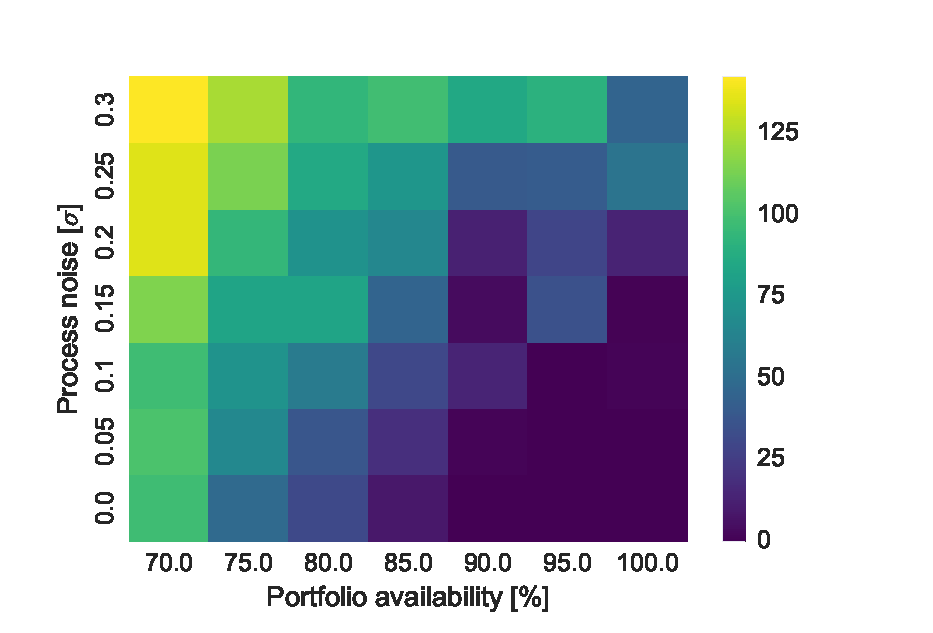
\includegraphics[width=\columnwidth]{figures/heatmap.eps}
%\caption{The RMS value over the test space. It can be seen that it is more important to have certainty in the portfolio availability than in the process noise.}
%\label{fig:colormap}
%\end{figure}

%\section{Quality Metrics}

What aspects of the aggregator influence in the performance metrics?

Internal vs. external metrics: external can be used for monitoring, internal can only manipulated in test environment.

Are there more metrics than in the table? E.g. robustness toward grid faults

\begin{table}[!t]%% increase table row spacing, adjust to taste
\renewcommand{\arraystretch}{1.3}
% if using array.sty, it might be a good idea to tweak the value of
% \extrarowheight as needed to properly center the text within the cells
\caption{System interactions can be evaluated with generalized metrics}
\label{tab:metrics}
\centering
% Some packages, such as MDW tools, offer better commands for making tables
% than the plain LaTeX2e tabular which is used here.
\begin{tabular}{ll}
\toprule
System interaction & metrics\\
\midrule
Aggregator - power system & responsiveness w.r.t. grid conditions\\
\\
Aggregator - DER portfolio & responsiveness w.r.t. time\\
 & robustness w.r.t. forecast errors\\
 \\
Aggregator -  ICT infrastructure & robustness w.r.t. communication faults\\
\bottomrule
\end{tabular}
\end{table}

\begin{table}[!t]
\renewcommand{\arraystretch}{1.3}
\caption{The quality metrics can be separated into two categories.}
\label{tab:metricsclass}
\centering
\begin{tabular}{ll}
\toprule
External metrics & Internal metrics\\
\midrule
responsiveness w.r.t. grid &robustness w.r.t. forecast errors\\
responsiveness w.r.t. time & robustness w.r.t. communication errors\\
& robustness w.r.t. grid errors\\
\bottomrule
\end{tabular}
\end{table}

\section{Discussion}
Specific terminology has been introduced to describe the proposed method. This terminology can be mapped to that of the field of \emph{Design of Experiments}, e.g. \emph{definition of service requirements} maps to \emph{definition of inner-noise factor} and \emph{definition of test inputs} maps to \emph{definition of outer-noise factors}. Specifically, the method resembles \emph{fractional factorial methods for off-line quality control}, see e.g.\cite{oehlert2010first}. In the case study presented in Sec.~\ref{sec:casestudy}, the inner factor, or controllable variable, is kept at a single level, i.e. the same activation signal is sent to the aggregator for each run of the experiment. The two outer factors, or noise variables, were varied over a distribution dictated by the operational scenario, i.e. the availability of the portfolio was varied on seven levels and, likewise, the process noise in the house simulation models was varied on seven levels. An important contribution of this work is applying this kind of formal test procedures to the problem of aggregator validation. The field of Design of Experiments is broad, and a further revision on the topic may yield a better method proposals than the one proposed here.

In this paper we focus only on the two  uncertainty sources mentioned above, therefore the test for time responsiveness, i.e. delay in the communications systems between the aggregator and a DER is not considered. This means that the test design presented in the case study is a simplified version of what an actual aggregator validation test would require. Future research must identify the relevant variables that need to be tested under the relevant operation scenarios. 

In comparison with the traditional test method, this validation procedure must capture the capabilities of a much more complex system, and therefore relies in part on simulations. As presented in \cite{steinbrink2015challenges}, the error between the used models and reality must be quantified and taken into account for the final aggregator certification. Each block in the simulation must use validated models or software. This applies to the communication systems, the grid models and the DER models. The test architecture, e.g. the one presented in \cite{buscher2015towards}, which validates the aggregators must also be validated.

There are still several open issues that need to be investigated with regards to aggregator validation. For example, the definition of the operation scenarios was only briefly discussed, and heuristics must be developed in order to define scenarios that are effective when testing aggregators.

Aggregator validation must be an ongoing process, that should be carried out periodically or whenever the aggregator portfolio or architecture changes significantly. Furthermore, aggregators are expected to participate in different electricity markets. Due to these reasons, along with the complexity of designing appropriate simulations, we believe that the task of validating aggregators should not carried out by the system operators, but by an independent third party. 
\section{Conclusion}
This work presents an initial approach to establishing a method for designing aggregator validation tests. This method differs from the traditional generator certification tests in that it relies on a statistical approach. Specifically, it reinterprets the generator certification tests to aggregators by adapting concepts from statistical testing to the problem. The validation test must be carried out with the aid of simulations, so that the stochasticity of the real world disturbances affecting the aggregator can be taken into account. 

While several of the concepts that form the proposed validation procedure, e.g. software framework for aggregator tests and aggregator performance assessment, have been addressed before, this work describes how these concepts can be unified in order to do a systematic testing of aggregators.

The validation procedure was shown through a simplified case study on an existing aggregator design. While the example shows a fictive setup, it appropriately represents the procedure.

An important step for the development of the validation method is the implementation of a complete test architecture with validated component models. With such a simulation framework, with realistic communication and DER models, communication delays can be implemented in order to test aggregators for time responsiveness. 

We consider the work presented here an important element of enabling aggregators in the smart grid, thus enabling consumption to actively participate in the secure operation of the power system. This will help the integration of renewable energy sources into the power system.



\chapter{Redefining Requirements of Ancillary Services for Technology Agnostic
Sources}\label{app:ddras}

\textbf{Authors:}\\
	Daniel~Esteban~Morales~Bondy\\
	Jason~S.~MacDonald\\
	Emre~C.~Kara\\
	Oliver~Gehrke\\
	Kai~Heussen\\
	S{\i}la~K{\i}l{\i}\c{c}\c{c}ote\\
	Henrik~W.~Bindner

\noindent
\textbf{Published at:}\\
Draft

\noindent
	\textbf{Abstract:}\\
Main points of the paper:
\begin{itemize}
\item DR and other technologies have unused potential that TSOs are not utilizing
\item This sub-optimality is due to current requirements oriented towards the lowest common denominator
\item Two options for optimal utilization of new resources: split market or unify under new conditions
\item We choose to unify by parametrizing the service definitions/requirements
\end{itemize}

\section{Introduction}

%Question: \emph{Who} are we going to convince of \emph{what}, and \emph{how}?\\
The requirements for ancillary services (AS) in many countries are defined, due to historical reasons, on the assumption that only generators provide ancillary services. With the increase in adoption of distributed energy resources (DERs) and controllable smart loads, as well as the emergence of schemes for utilizing consumption flexibility, such as demand response (DR), new sources for ancillary services from the demand-side are available. 
These sources posses qualities that in many cases match the performance needs of the system better than traditional generators, yet their participation in the ancillary service markets is restricted due to requirements barriers. Since there are both economic and technical benefits in exploiting these qualities, a method must be designed so that system operators can readily utilize the positive qualities of both traditional and new ancillary services sources. In this paper we propose new frequency ancillary service requirements, focused on service performance, which are source/technology independent. 

By changing the AS requirements to focus on performance rather than unit capabilities and utilizing new technologies as ancillary service providers, system operators will be able to maintain better system reliability\cite{entsoe2014demand}, and increase participation in the ancillary service markets. Furthermore, service verification and settlement will benefit those players that are able to provide better quality services.

The rest of the paper is organized as follows: section~\ref{sec:currentas} presents the current ancillary service definitions and requirements; section~\ref{sec:newas} presents the new ancillary service requirements; section~\ref{sec:ancsrvDR} presents the performance properties of different new technologies that make them suitable for frequency ancillary service provision. Section~\ref{sec:ddrascasestudy} presents a case study of the impact of the new requirements, and section~\ref{sec:ddrasconclusion} presents conclusions and thoughts for future research. 

%\begin{itemize}
%	\item Increase of fluctuating RES and aging infrastructure lead to need for AS
%	\item ``Square peg in round hole'' problem
%	\item Why:
%		\begin{enumerate}
%			\item Help the system operators get the maximum out of the properties of DR, leading to better system balance/stability/reliability, see \cite{entsoe2014demand}
%			\item Incentive new players/aggregators in the energy markets by providing fair remuneration (paid for what DR can do, not for behaving like a traditional generator)
%			\item Ease verification and settlement of DR services (related to the previous point)
%		\end{enumerate}
%\end{itemize}



\section{Ancillary Services: Current Definitions and Requirements}
\label{sec:currentas}

The objective of ancillary services can generally be defined as: maintaining an adequate and secure power system. This means maintaining the power system operating at nominal frequency and voltage. In cases where the power system deviates from nominal operation, either due to natural fluctuations in consumption or faults in the system, the system operators will activate ancillary services to restore normal operation.


%%%%%%%%%%%%%%%%%%%%%%%
\subsection{The function of ancillary services}
%%%%%%%%%%%%%%%%%%%%%%%
%\textcolor{red}{We want to describe what is the purpose of the AS that are within scope, and describe which physical need they are covering}

In the electricity system, supply and demand must be kept balanced at all times and two metrics are commonly used to evaluate the current imbalance in a power system: system frequency and the area control error (ACE). System frequency is a measure of the speed at which all interconnected, synchronous generators are rotating.  ACE is a measure of the deviation in scheduled power exchanges between interconnected electricity systems. 

System imbalances have two causes:
\begin{enumerate}
\item Expected imbalances due to deviations between the planned generation and the actual electricity demand.
\item Unexpected imbalances due to system contingency.
\end{enumerate}

System operators procure ancillary services\footnote{Ancillary services are also used to solve other operating issues in the power system, such as voltage problems, but this work will focus specifically on frequency services.} in order to deal with these imbalances in their daily operation. The structure of the ancillary services varies between systems but can generally be divided into primary, secondary and tertiary control\footnote{Recently, ENTSO-E has changed its terminology for AS providing Load-Frequency Control to Frequency Containment Reserves, Frequency Restoration Reserves (either automatic or manual), and Replacement Reserves\cite{entsoe2013network}. This classification matches roughly into the framework presented in \cite{Rebours}.}\cite{Rebours}. This work will focus specifically on the primary and secondary frequency control.

\subsection*{Primary Frequency Control}
Primary frequency control is the fastest response (in the seconds range) and is used to arrest and begin reversing frequency excursions occurring due to sudden imbalances between supply and demand, often caused by contingency events. Primary frequency control is traditionally performed by generators under ``droop'' control, in which a  change in power output is made proportional to locally measured frequency. The reason for this is that the response to the frequency excursion must occur as fast as possible and be proportional to the size of the excursion so that the system frequency stabilizes within an acceptable time frame.
\subsection*{Secondary Frequency Control}
Secondary frequency control is a slower response (in the seconds to minute range) that takes over for the primary frequency control and returns the system to nominal frequency by controlling the output of participating resources. Much more urgently, it restores the full bipolar range of the primary reserve, so the system gets back to nominal $n-1$ redundancy. Usually an entity estimates the control reference signals based upon the ACE and system frequency to simultaneously resolve the imbalance at the interconnection and maintain stable operation (see, e.g. \cite{nerc2011balancing,entsoe2014continental}, for more details). The control algorithm that directly controls the output of resources providing this service is often called Automatic Generation Control (AGC)\footnote{This balancing control logic can have a centralized, pluralistic or hierarchical architecture~\cite{entsoe2014continental} to determine the individual reference signals for the generators.}. The generators will have either a proportional controller or a proportional-integral (PI) controller to track the AGC signal. The secondary response also needs to occur as fast as possible, yet due to its centralised control approach, it is not able to provide as fast a response as primary control. The underlying need for the secondary service is to supply a fast reference tracking response without overshoot.



\subsection*{Addressing the need}
%\olge{This section duplicates quite a lot of information from the previous one. Maybe they could be joined?}
An illustration of the power system frequency during a contingency is shown in Fig.~\ref{fig:contingency}. When a system contingency occurs, such as the loss of a large generator or a transmission line, there is a sudden loss in generation that is made up for by the small amount of inherent storage in the rotating inertia of the remaining synchronous generators. This sudden loss reduces the rotational speed of said generators which results in a frequency excursion whose slope is determined by the total inertia of the system. The inertia of the system is determined by the amount of kinetic energy in the synchronous generators in the system, and as these generators are decommissioned, the inertia in the system will decrease, thus increasing the volatility of the system. Until now, system operators have been able to arrest frequency excursions fast enough because of the inherent system inertia, but as the inertia decreases, faster response times are required of the primary frequency control. 

The system operator must have enough primary reserves to arrest the frequency as fast as possible, before the system enters a state where a blackout is inevitable. A metric for how effective the procurement of reserve is the \emph{frequency nadir} \cite{eto2010use}, and it is desirable that the value is as close as possible to the nominal frequency of the system.

Similarly, the system operator should ensure that the secondary reserves act as fast as possible to relieve the primary reserves and also bring the frequency from the settling frequency back to the nominal frequency.

In \cite{vrettos2015integrating} it is shown that if primary frequency response is provided by demand response (with a very fast response), the frequency nadir occurs at higher frequencies. 
Also, in \cite{makarov2008assessing}, the authors argue that the value of regulation resources can be defined based upon the ramp capabilities of the service providing units. Faster reacting units are more valuable to system operators, since they help arrest the frequency excursion faster and at a higher nadir. It does require changes to the AGC in order to utilize the fast response, but this would also lead to the need for fewer reserves.

\begin{figure}[htbp!]
\centering
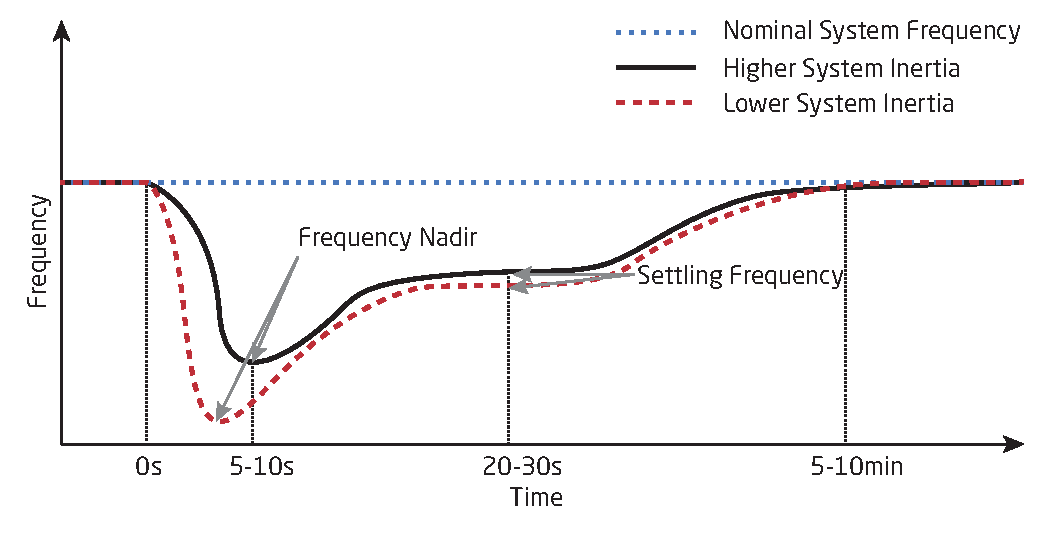
\includegraphics[width=1\columnwidth]{frequency_contingency.eps}
\caption{The nadir of a system frequency excursion during contingency events is more pronounced if there is less inertia in the system.}
\label{fig:contingency}
\end{figure}

%%%%%%%%%%%%%%%%%%%%%%%
\subsection{Ancillary service procurement and service  requirements}\label{sec:procurement}
%%%%%%%%%%%%%%%%%%%%%%
%\textcolor{red}{we talked about the needs, they are tackled by the following requirements, due to historical, computational reasons. Here it should be made clear in which way the current requirements do not exploit the full capabilities of all units}

\subsection*{Procurement requirements}
All electrical power systems require ancillary services, but not all system operators acquire them through market mechanisms. In the US, primary frequency control is expected to be part of the normal operation of the generators, and is therefore not directly compensated. In other cases, AS are bundled within bilateral energy contracts as one product contracted by the system operator.

In all instances, the system operators have procurement requirements that are dimensioned through static analysis of the system. Until recently, measurement equipment has not been able to measure the frequency nadir\cite{eto2010use}. Consequently, the dimensioning of the primary reserves has been made on the settling frequency, parting from static offline calculations of the dynamics of the grid. Typically, system operators are required to contract reserves corresponding to a percentage of the overall system load, e.g. regulation reserves usually cover 1\% of the load, or cover the loss of specific units, e.g. the \emph{N-1} criteria.


\subsection*{Service Requirements}
Because AS are essential for the secure operation of the system, the system operators also have requirements and restrictions on the units providing AS. A super-set of requirements across different systems is defined in \cite{Rebours}. These requirements can roughly be classified into three categories: \emph{temporal requirements}, which relate to how fast and for how long a service must be delivered; \emph{resource tuning requirements}, which relate to specific values that tuning parameters in the resource must have; and \emph{market requirements}, which relate to bid sizes and similar parameters in systems where services are acquired through market mechanisms. Of these three categories, only the temporal requirements relate to service performance. Furthermore, in most systems are the requirements implicitly defined for traditional generation units. This means that most service requirements are oriented towards the least common denominator of service providers, e.g. a unit providing primary frequency control should provide half of the service within 15 seconds and full response within 30 seconds\cite{energinet2012ancillary}. A variety of generation and consumption units would be able to provide this service faster, but this quality is not rewarded. Another example is the requirement of having a PI-controller on units providing secondary frequency control, in order to track the AGC signal. Such a controller is infeasible on distributed systems, but other modern controllers can provide offset-free control with similar properties.


%Units which do not perform within the specified requirements are heavily fined. \macd{I assume there will be more to follow this statement?}\bondy{Yeah, I had hoped you might want to write a line or two here :-).}
%\textcolor{red}{Joe wants us to go much more in depth on this point, for example discuss how PJM has reg A and D}
%
\subsection*{Impacts of historical requirements}

%\bondy{(The following section should make it clear why the new resources would be utilized suboptimally if they have to comply to current requirements. I'm having problems tackling this section, perhaps Kai and Jason could help?, also, the title of the section should perhaps be changed?)} \macd{Perhaps the title of this section should be "Impacts of historical requirements", or something like that. }

In short, the historical definitions for service requirements results in the suboptimal use of today's AS resources. Due to the legacy definitions there is an implicit %explicit 
bias for traditional resources, and alternative technologies, such as demand response, are are restricted in their contribution to AS provision, and their favorable properties are not utilized or undervalued.

While system operators have been able to maintain a secure system using traditional resources, the changes in the power system, i.e. the decrease of system inertia and increased fluctuation due to RES, require units that react faster than the current minimum requirements. Also, an increased overall volume of balancing resources will be required due to the larger deviations caused by the RES.
Units that provide a faster response but are not able to provide the full response duration should be enabled to contribute to AS provision and be valued accordingly.

If these technologies, both the underutilized and the ones restricted from providing services, are used optimally for ancillary service delivery, it follows from the conclusions presented in \cite{makarov2008assessing,vrettos2015integrating} that frequency excursions could be arrested at higher frequency nadir, thus lessening the required amount of reserves, which leads to a lower-cost operation of the system. 
Regulative authorities have concluded that fast reacting units are valuable for the system operation, and started programs to benefit of these resources. An example of this is FERC order 755 (Pay for Performance) which has led to PJM splitting their regulation market product into RegA, for slow reacting units, and RegD for fast reacting units. The product differentiation approach has been a success for PJM, but splitting the market into different products does not address two points: 1) the overall pool of resources will not be optimally utilized, and 2) as other new technologies appear in the system, the market might fragment further, also leading to non-optimal utilization of resources.  We propose instead to restructure the ancillary service definitions such that all types of service providers participate with the same market product defined by a set of optimal performance parameters, and not by minimum requirements. This means that the all entities providing a given ancillary service, e.g. primary frequency control, are optimally cleared under a single market. The service restructuring is detailed in the following section.


\section{Unconventional Resources}
\label{sec:ancsrvDR}

\subsection{Related Work}
There is growing evidence that demand-side resources (DSRs) can participate in ancillary services, thus substituting the need for traditional ancillary service resources. However, the DSRs that can provide ancillary services vary greatly in composition, and have distinct properties. Most of the research on DSRs to provide transmission-level services has focused on specific services using a particular set of loads connected to the grid. This is partly due to varying characteristics of DSRs and partly to the suitable control architecture for the proposed services. 

A common set of resources studied in connection to DR are thermostatically controlled loads~\cite{Molina_Garcia_2011,Kara_2012,thavlov2014utilization,mathieu2012using}, such as electric space heating \cite{mathieu2012using,thavlov2014utilization}, residential and industrial refrigeration \cite{lakshmanan2014energy}, and space heating using heat pumps \cite{halvgaard2012economic}. Thermostatically controlled loads are valued for their ability to provide ancillary services because of the inherent thermal inertia present in the systems. The thermal inertia acts as energy storage, permitting the curtailment or deferral of power consumption. The application of TCLs as a DR mechanism can also be seen in industrial settings such as large refrigeration systems \cite{rahnama2013integration}, the heating of bitumen tanks \cite{cheng2014availability}, and indoor climate control using HVAC \cite{blum2013ancillary}. 

Batteries can also provide ancillary services through demand response. Electric vehicles (EVs) can be considered as mobile batteries with additional time varying constraints. By changing their charge patterns while guaranteeing the mobility needs of the owner, EVs can offer the demand-side flexibility needed to provide ancillary services to the grid \cite{zarogiannis2014dynamic,kara2015estimating}. 

The potential of using the dimming of lighting in office buildings for DR is presented in \cite{rubinstein2011demand}. A pilot project in Denmark also used the lighting system in an industrial green house for DR, showing the potential of using DR to manage congestion in the distribution system. 

Water pumps--used in wastewater treatment systems and agriculture--are also considered a promising resource for ancillary services. Specifically, in \cite{halvgaard2014waste}, the authors suggest that water can be temporarily stored in pipes and tanks, hence delaying the transportation for treatment in waste water treatment systems. The load flexibility of agricultural water pumps stems from the inherent flexibility in the time of irrigation.
%The response of the pumps is fast, and depending on the system state and weather conditions can be sustained from medium to long time. The system requires a certain amount of energy to move the water around, and is therefore deferrable. Due to the pumps there may be constraints on the cycling.
%Furthermore, 50\% of the energy consumption of a waste water treatment plant is spent on the aeration process, which can also be deferred. 

In this paper, we examine the use of DR when system reliability is jeopardized. A great deal of research has focused on DSR-specific controller design and limitations due to load characteristics and comfort needs. Specifically, many aggregation frameworks exist in the literature that overcome cycling constraints and response frequency limitations. Hence, instead of focusing on the design of such DSR-specific controllers, we assume that AS provided by DSRs will be sold to system operators by an aggregator, and that the aggregator is responsible for control accuracy. 
Our objective in this paper is to discuss and formulate ideal performance requirements for ancillary services in a number of relevant features, and to provide a market clearing mechanism that selects a portfolio of resources in a resource-agnostic and performance-oriented way. By doing so, we propose a strategy in which (i) we remove the barriers preventing unconventional resources from participating in AS markets due to the static nature of AS market definitions and requirements, and (ii) we provide a fair and performance-based market clearing structure in which the unused potential of DSRs can be easily incorporated.

\subsection{Properties}
The identified DSR parameters are given as follows:
%\kara{I think here we need a discussion of parameters that we are using in Section 4 to define $\kappa$} \kara{I think the properties should be of aggregations, not necessarily the DR resources}
%\olge{I know I probably spend way too much time looking at microcontroller timing diagrams, but would it help trying to put all the parameters into a single timeline drawing like the sketch in figure {\ref{fig:resourcecharacteristics}} ?}
%\begin{figure}[htb!]
%\centering
%\includegraphics[width=1\columnwidth]{20150731150249153.pdf}
%\caption{Characteristics of demand side resource [sketch].}
%\label{fig:resourcecharacteristics}
%\end{figure}

\begin{description}
    \item[Response time] This is the time it,takes for a unit to receive a DR signal and react upon it. %\textcolor{red}{I'm not sure on this one, since pretty much all of them have fast response time, depending on the control architecture and the communication system, which are not inherent to the DER}
    \item[Response duration] How long is a pool of these units able to sustain service provision: short, medium or long. %\textcolor{red}{Again, this is a tough one, since this will depend on the state of the portfolio/unit}
    \item[Response magnitude] This the \emph{amount} of load used by the DR resources that can be increased or decreased. The increase capability is defined as the \emph{take} magnitude and the decrease capability is defined as the \emph{shed} magnitude.
\end{description}


\subsection{Unused Potential of DSRs and Barriers to DSR Participation}

\label{subsec:unused}
Although DSRs provide additional freedom to help shape response compared to traditional AS providers, the existing ancillary service market rules and requirements are a strong barrier to DSR market participation. A recent study identifies such barriers in the US\cite{cappers2013assessment}. The rules and requirements that limit resource participation in different markets are not consistent among different RTOs and ISOs; however, the authors identify three major groups of these rules: rules on the size of the resource, rules on the measurement and telemetry of the resource, and rules on market bidding time. Out of six different ISOs and RTOs in the US, only one allows load aggregations to provide regulation services, and only two allow aggregation participation as a spinning reserve provider. Furthermore, only two ISOs and RTOs allow aggregate telemetry. Providing telemetry at an individual resource level increases the overall cost of metering, making it challenging for DSRs to provide cost-competitive AS. Finally, most of the AS markets procure in day-ahead markets, and day-ahead DSR participation is harder due to increasing uncertainty in DSR flexibility forecasts.  

In order to accommodate the slow-ramping resources as well as DSRs in the AS markets, there is an increasing need to either split AS into different service classes or parametrize the service definition so that the resources are selected only by their ability to satisfy the system needs. The ideal resource to satisfy the system need is one with ``unlimited capabilities in terms of response time, energy output, ability to frequently reverse their output, ability to respond and follow the AGC setpoint changes, and size.''\cite{makarov2008assessing}\footnote{For this kind of response to be optimal, changes must be made to the AGC algorithm \cite{peydayesh2012effects}.} To include and incentivize the participation of technologies that in some parameters are closer to the ideal than those defined by the current service and market requirements, two methods can be utilized: product differentiation and product restructuring.

Some transmission system operators, like PJM, have already suggested that better service performance is more valuable than simply adhering to traditional rules and requirements, and split their regulation market into a slow service product and a fast service product. 
This work explores the alternative: restructuring the market so that all technologies can participate in the same market, and the system operator can optimize the use of the resources based upon their capabilities. This entails reformulating the temporal and market requirements, and removing the requirements that implicitly assume that the services are provided by traditional generators, thus making the requirements technology-agnostic. %In the next section, we discuss the \emph{new proposition}.\kara{to be filled} 


 

\section{Restructuring the Ancillary Service Requirements}
\label{sec:newas}
\subsection{Overall approach}
%[argument vs. current approaches start supporting performance of new resources by a more lenient apporach blb bla cut it]
%\kh{Guys, we really have to clarify the workding of 'performance': in performance-based remuneration, the 'performance' is a 'quality of execution' (Sect. 4.4 $\eta^{AS}$); however, our $\kappa$ does not look at 'performance' but rather at a 'quality of shape' (lacking a better word to describe the 'fitness' assessment quantified by $\kappa$.)}

%The key idea of the proposed approach is to formulate ideal performance requirements for each ancillary service in a number of relevant features, and then to provide a market mechanism that allows to define an optimal control resource portfolio building on beneficial combinations accounting for complementary properties of control resources. 
The proposed restructuring assumes that system operators acquire AS reserves through a market, and that potential AS providers bid their reserve capacity in that market. The restructuring is based on the following four key concepts (which are expanded upon throughout this section):
\begin{itemize}
    \item The formulation of an \emph{ideal ancillary service response} that the system operator desires for the system. This formulation will be strongly dependent on the needs of the system operator, e.g. very fast response in case of low system inertia, and will be submitted as a tender to the market.
    \item The \emph{parametrization of the AS bids}, where the parameters reflect the service providers' capabilities to partially fulfill the ideal service response. This removes the minimum-requirements-barriers on new technologies, thus enabling any useful unit to participate in the AS provision, which facilitates market liquidity.
    \item Clearing all units under a \emph{generalized single clearing-price auction}, provides incentives to bid actual marginal cost. In this auction, the capability value of each service provider and their historical performance is taken into account.
    \item \emph{Performance-based remuneration} gives incentive to better AS provision and enables transparent performance-based clearing of the market.
\end{itemize}
%to formulate an ideal tender requirements for each ancillary service, based upon a number of key parameters that directly address the system needs\bondy{fix}. Since current market mechanisms implicitly rely on a homogeneous set of responses, a proposal for a new market mechanism is presented, which allows to define an optimal control resource portfolio. The portfolio is built on optimal combinations of the resource key parameters, accounting for complementary properties of the resources, and seeks to minimize the cost of the reserve while ensuring that the overall response of the portfolio is optimal with respect to the service needs\bondy{fix to minimum capability tender}. 

%performance is thus embedded in present ancillary service definitions assumes only the exact following of the service is beneficial to the system - on the contrary actually resources may have dynamics that complement each other.
%essentially ...
%((linear) combination of heterogeneous portfolio)
%vs. 
%(scalar decomposition of homogeneous portfolio)

%ARGUMENTS:

%(1) The \textit{parametrization of AS bids} removes minimum requirements, enabling any 'useful' unit to participate (facilitates market liquidity, removing barriers for demand response participation);
%(2) A generalized \textit{single clearing-price auction}  providing incentives to bid actual marginal cost.
% REF for now: https://www.epsa.org/forms/documents/DocumentFormPublic/view?id=F64F00000033 and
%(3) \textit{Performance-based remuneration} incentivizes better service and enables transparent performance-based clearing;

Based on an assessment of the complete decision process, we merge the four key concepts outlined before into a novel approach to ancillary service valuation that accounts both for performance of resources and the actual spectrum of system needs.  % The actual market clearing is then
The holistic assessment includes:
\begin{itemize}
	\item \textit{Planning}: Assessment of system need, parametrization of resource performance and specification of tender conditions.

	\item \textit{Scheduling}: Quantification of AS tender volume, AS bid submission, and market clearing.

	\item \textit{Operation}: Reserves dispatch/activation and monitoring.

	\item \textit{Settlement}: Verification of service delivery and remuneration.
\end{itemize}

As outlined above, for effective inclusion of DR (or any other unconventional resource) in AS markets, a revision of each phase is required. Our proposal focuses on a new \textit{parametrization of services} (Sec.~\ref{subsec:parametrization}), which affects in particular \textit{market clearing} (Sec.~\ref{subsec:marketmechanism}) and \textit{remuneration} (Sec.~\ref{subsec:performanceremuneration}). 

In Section~\ref{sec:ddrascasestudy} we illustrate the impact of this reformulation in comparison with present market mechanisms, and in \ref{sec:ddrasdiscussion}, the alignment with present mechanisms and its applicability to novel ancillary service models (REF WARRINGTON/policy based) is reflected.  

\subsection{Ideal service tender}\label{subsec:idealtender}
The ideal source for AS is one with ``unlimited capabilities in terms of response time, energy output, ability to frequently reverse their output, ability to respond and follow the AGC setpoint changes, and size .''\cite{makarov2008assessing}\footnote{For this kind of response to be optimal, changes must be made to the AGC algorithm \cite{peydayesh2012effects}.} It is impossible for any one unit to possess these characteristics, but system operators aim at achieving this kind of system response by contracting several units.

In existing AS, there is an implicit assumption that ideal unit response corresponds to a scalar fraction of the required system response. In contrast, in presence of a diverse resource portfolio, the commonly expected fast response is secondary to an overall cheaper mixed portfolio which delivers a better system response, e.g. by combination of a fast duration-limited and slower unlimited response time resources.

%\kh{What is the difference between conventional dimensioning (see "operations manual") and dimensioning with capability parametrization?}

For example, a system operator could determine that the ideal system response to a frequency excursion is the one that has a resulting frequency nadir at the settling frequency (thus minimizing the risk of tripping the under-frequency relays). Based upon the inertia in its system, the system operator determines the volume ($V_{tot})$ needed as well as the response characteristics needed to achieve this, see Figure~\ref{fig:ddrasidealresponse}.

\begin{figure}[htbp!]
\centering
\includegraphics[width=1\columnwidth]{graphics/ddras/primary_frequency_control_ideal.eps}
\caption{In this case, the ramp of the ideal response is mainly determined by the system inertia and is to be sustained until secondary frequency control can be activated.}
\label{fig:ddrasidealresponse}
\end{figure}
%%4.2
%* bid formulation uses simplified constraints that can be addressed both for conventional generation and are also straightforward to be formulated as response capability of a diverse DR portfolio;

\subsection{Parametrization of service performance}\label{subsec:parametrization}

Ancillary service requirements are specified by a system operator based on the desired control response for a particular power system. Today, these requirements --- as reflected in the service definition --- are not differentiated according to the capabilities of the unit providing the service. Therefore, service definitions are designed to accommodate the least capable unit in the portfolio. As a consequence, more capable units are not being fully utilized, leading to excess contracting of service providers.
This suboptimal allocation of resources could be addressed by introducing a performance dependent definition of ancillary services, i.e. a service definition which allows compliance to be measured on a linear rather than a binary scale: In addition to compliance and noncompliance, different levels of partial compliance are possible.
In this context, services will be defined such that the best possible performance of the most capable unit corresponds to full compliance. The overall ideal service requirements can be expressed as:
\begin{equation}
	S^* = f_m(\textbf{x}^*) \label{eq:ddrasoptimaltender}
\end{equation}
where $\textbf{x}^*$ is a vector of ideal parameter values and $f_m(\cdot)$ a function that translates the parameters $\textbf{x}$ into a model. Furthermore, the system operator must inform how the parameters are valued with respect to the $S^*$, which is done through a capability value:
\begin{align}
    \kappa &= g(\mathbf{x}) \\
    \kappa &\in [0,1].
\end{align}

AS aggregator bids submitted include: 
\begin{itemize}
\item offered service parameters: $\mathbf{x}$
\item bid price: $P^{bid}$
\item (for cross-validation) estimated: $\kappa$
\item unit quantity (volume): \emph{V}
\end{itemize}

The bid parameters are service-specific and serve both for market-clearing and performance calculation. 

%%4.3
\subsection{Market mechanism}\label{subsec:marketmechanism}

In order to leverage the proposed AS restructuring, the market clearing mechanism needs to be changed. The clearing should take the \emph{capability value} of the service providers into account, and ideally also the probability of availability (certainty in service). There are many different ways of formulating such a market clearing mechanism and here we present an example of a market that utilizes the service parametrization to form an ideal service response.

The market is designed as a single clearing price auction, in which each resource bid is adjusted by \textit{two} factors for bid quality: 1) a shape-matching parameter $\kappa_i$ and 2) a historic performance  parameter $\eta^{hist}_i$.
%The benefit of the merit order is that by remuneration at clearing price it provides competitive incentive for bidding with true marginal cost 
The clearing mechanism identifies a common clearing price based on the most expensive accepted bid. 
%Clearing principles
\begin{equation}
    P^\mathtt{clear} = \max P^\mathtt{bid}_i, \quad i \in \Omega^\mathtt{acc}
\end{equation}
where $\Omega^{acc}\subseteq \Omega$ is the subset of accepted bids of the set of received bids $\Omega$. 
The clearing mechanism selects the subset of bids which offer the cheapest overall clearing cost and meet the tender requirements: 
\begin{align}
      \Omega^\mathtt{acc} &= &\mathtt{argmin}_{\Omega^\mathtt{hyp} \in \mathcal P(\Omega)} \sum_{i\in \Omega^\mathtt{hyp}}{\kappa_i P^\mathtt{clear}_{\Omega^\mathtt{hyp}} } & \\
      &\mathtt{s.t.}& \sum_{i\in \Omega^\mathtt{hyp}} V_{i}\ge V_{tot} &  \\
      &~ & \eta^{hist}_i \geq \eta^{hist}_{min} &\quad \forall i \in \Omega^\mathtt{hyp} \\
      &~ &\sum_{i\in \Omega^\mathtt{hyp}}{\eta_i V_i}/V_{tot} \geq \eta^{AS}& 
\end{align}
Where $\mathcal P(\Omega)$ denotes the Power Set of $\Omega$.
%As both tender specification and bid parametrization correspond to a $n$-dimensional polygons, the bids can be summed up and the sum can be compared to the tender polygon.

The specification of tender and bid parametrization needs to be aligned with the mechanisms applied during real-time operation the resource dispatch and activation.
Resource performance is monitored with respect to the behaviour expected from bid parametrization, and is further expanded upon in the next subsection.




%%4.4
\subsection{Performance-based remuneration}\label{subsec:performanceremuneration}
%\bondy{I write here}

%\bondy{3) adherence to performance model is evaluated and applied to base price}

Performance-based remuneration has already been introduced in United States through the FERC order 755. Similarly, in this work we propose that service providers are paid according to how close they follow the capability parameters they bid to the market. The estimation of the service provision performance can be done in different ways, depending on which parameters the system operator deems to be the most critical. A service performance index is proposed in \cite{bondy2016method}, where service performance is defined as the root mean square error of the actual service delivery compared to the ideal model:
 \begin{align}
     \eta^{post} &= \sqrt{\frac{\sum^{N}_{t=0} \left( {QoS_{t}}^{2} \right)}{N}},\\
     \eta^{post} & \in [0,1],
 \end{align}
 where \emph{N} is the time horizon over which the service is delivered and $QoS \in [0,1]$ is the \emph{Quality of Service} of the ancillary service, which is the error in service delivery scaled to the tolerance limits defined by the system operator. This leads to the final settlement price of service provision being defined as:
\begin{equation}
    P^\mathtt{rem}_i = \eta^{post}_i\kappa_i  P^\mathtt{clear} \qquad \forall i \in \Omega^\mathtt{acc}.
\end{equation}
 


%\section{Case study}
%\label{sec:newas}
%
\subsection{Case 1: Primary Frequency Control}
For example, for primary frequency control, which expects a step response from a nominal set-point to a new set-point based upon the frequency deviation, the TSO needs to establish two parameters:
\begin{itemize}
\item Optimal ramp time per bid atom
\item Optimal service duration
\end{itemize}

The optimal ramp time needs to be defined by the TSO, and will be derived from the inertia of the system. For example, the Danish TSO could determine that the optimal ramp time to be 0.001 s.

The optimal service duration depends solely on how fast it is able to activate secondary reserves. Again, in the Danish case 15 minutes is chosen to be the optimum.

Thus the performance value of units expecting to provide primary frequency control services can be characterised by:
\begin{align}
\kappa &= \alpha_1 \frac{\tau_{r,0}}{\max({\tau_{r,0},\tau_{r,a})}} + \alpha_2  \frac{\min(\tau_0,\tau_{a})}{\tau_{0}}\label{eq:kappa_primfreq}\\
\sum_{i} \alpha_i &= 1
\end{align}
where $\tau_{r,a}$ is the actual ramping time that the AS-providers can deliver, $\tau_{r,0}$ is the optimal ramping rate that the TSO would like to have. Similarly, $\tau_a$ is the endurance time that providers can deliver, and $\tau_{0}$ the the ideal endurance time the TSO would like. 
The TSO can assign a priority to any of the two variables by adjusting the weight factor $\alpha \in [0,1]$.

The formulation of equation~\eqref{eq:kappa_primfreq} has the property that a fast responding/short endurance service provider may be as valuable as a slow responding/long endurance service provider. 

\subsection{Case 2: Load Frequency Control}

E.g. for AGC/regulation/LFC:

1) The system requirements for the AS are: 
\kh{Esteban, what's the numbers again? cheers}
\begin{itemize}
\item Maximum ramp time for procurement volume $\tau_r$
\item Maximum activation time for 5\% procurement volume $\tau_{r5}$
\item Expected (minimum) duration of service $\tau_E$
\end{itemize}

2) \textbf{Tender:}
$P_{R,tot}$ total volume

Bid Parameters: 
$P_{R,a}$ - bid volume, $R_{a}$ - ramp rate, $\tau_a$ - duration 
\kh{i am not sure if we should formulate the limit as 'energy' or as 'duration', as the effects are quite different in case of partial activation --kai}


Other Service properties:

Performance parameter:
\begin{align}
\kappa &= \alpha_1 \frac{\min({R_{0},R_a})}{R_0} + \alpha_2  \frac{\min(\tau_0,\tau_{a})}{\tau_{0}}\label{eq:kappa2}\\
\sum_i\alpha_i &=1
\end{align}

3) 

\begin{figure}[htb!]
\centering
\includegraphics[width=1\columnwidth]{utility_ramp_endurance.png}
\caption{Caption it yourself!}
\label{fig:utrend}
\end{figure}

%\section{Previous section 4}
%\label{sec:newas}
%

%\begin{itemize}
%	\item Is it possible to avoid the baseline problem?
%	\item Define services in terms of performance, not characteristics.
%	\end{itemize}
%Product definition(suggestions):
%		\begin{itemize}
%			\item fast response product (gets paid for delivering in full as fast as possible, over short time horizons)
%			\item sustained delivery product (gets paid for the time period it is able to fully deliver the service)
%		\end{itemize}
% AS on the aggregators/DERs terms (new requirements)\\ 
%Verification and Settlement

\bondy{1) Ideal ancillary services needs are established and product performance is directly derived from these needs in form of a scalar heuristic based on performance variables. % are directly related to the system need. % (not upon minimum requirements).
2) remuneration based upon optimal value of the scalar heuristic.
3) New service definition leads to a new market clearing mechanism.}

The ideal source for ancillary service is one with ``unlimited capabilities in terms of response time, energy output, ability to frequently reverse their output, ability to respond and follow the AGC setpoint changes, and size .''\cite{makarov2008assessing}\footnote{For this kind of response to be optimal, changes must be made to the AGC algorithm \cite{peydayesh2012effects}.} In order to include and give incentive to the participation of technologies that in some parameters are closer to the ideal than those defined by the current service and market requirements, two methods can be utilized: product differentiation or product restructuring.

Some transmission system operators, like PJM, have already introduced the idea that better service performance is more valuable\footnote{See RegA and RegD in [cite].}, and split their regulation market into slow service product and a fast service product. 

This work explores the alternative, that is, restructuring the market, such that all technologies can participate in the same market, and the system operator can optimize the use of the resources based upon their capabilities. This entails reformulating the temporal and market requirements, and removing the requirements that implicitly assume that the services are provided by traditional generators, thus making the requirements technology agnostic.

The new service requirements definitions

- PRIM derived from inertia and no overshoot beyond settling frequency \& duration derived from secondary response \\
-- dimensioning of primary reserve defines settling frequency

- SECO derived from (cost/resource-optimal) primary and desired frequency restoration time 

- TERT derived from time to response

%It is concluded in \cite{makarov2008assessing} that a generator providing ancillary services close to the ideal (i.e. with large ramping rates), are more efficient for arresting frequency excursions earlier, and are therefore more valuable. There is a system wide benefit in creating better market opportunities for fast responsive resources. But in some instances, units that are able to provide very fast responses are not able to sustain their response for the currently required length of time (\textcolor{red}{refer to Vestas example if published, or other relevant example}).\bondy{To do: This whole paragraph should be reformulated so that the parameters are more generic, according to the service} Therefore the value of a unit should not only be evaluated based upon its ramping time, but also its response endurance. This paper proposes a new way of expressing these two service requirements into a single value. 

\subsection{Service Performance Parametrization}
Resource model: 

 - PROPOSAL1: ramp rate (MW/min), delay(min), duration (min), power (MW)\\
 
VOLUME:  (duration-(delay+power/ramp))*power+1/2*power/ramp*power)
 
- PERF: RMSE(Ideal unit parameters - parameters of the volume brick)
 
 - PROPOSAL2: full response time, duration, power\\
 
 alpha1*duration + alpha2*power - alpha3*

\bondy{We need express the system needs through parameters. Bring in Figure 3 or similar}\\
indicators

defining perfectly (responding) resource characterization

"threshold response" - the minimally acceptable reserve provisions (the reserve need)



\subsection{Performance-based Remuneration}

\subsection{Service Procurement Process}
\textit{Step 1:} Ancillary service specification by System operator. A system operator defines the system requirements and objectives for a specific ancillary service. These requirements are primarily formulated in terms of minimum requirements for the overall response. 

\textit{Step 2:} (AS) Service tender conditions: 
The tender defines requested total service volume, bid parameters and a derived performance parameter $\kappa$. 

The bid parameters are service-specific and serve both for market-clearing and performance calculation. The parameters are chosen considering idealized response characteristics, simplicity of calculations, service needs, verifiability, (linearity?) \kh{[...tbd...] }
The performance parameter defines the trade-off between bid parameters. 

Also, the tender will specify the granularity of the bids, so there is a standard bid size, e.g. 1 kW, of which each player can bid several of. For example, if aggregator \emph{X} wants to sell 5 MW, it bids 5000 units of the service. In this way, each bid's performance value $\kappa$, and the parameters that conforms it, will be comparable.

Steps 1-2 apply define the market setup. Steps 3-7 apply to each tendering period. 

\textit{Step 3:} Bid formulation:
AS aggregator bids submitted include: 
\begin{itemize}
\item offered service parameters
\item bid price
\item (for cross-validation) estimated $\kappa$
\item unit quantity (volume)
\end{itemize}


\textit{Step 4:} Market Clearing: based on submitted bids and required procurement volume the market is cleared by incrementally increasing the pool. For each new block of bids added to the portfolio, a new tetris optimization is done by the TSO. When the minimum requirements to the service specifications is met, the market is finished/cleared.

outcome: procured reserve portfolio; market clearing price according to the highest cleared price.

[\textit{Step 5: }Activation]

[\textit{Step 6:} Verification]

\textit{Step 7:} Remuneration is based on the market clearing price and the performance parameter $\kappa$. 
$\$*volume * \kappa - penalty$
penalty if Bid specs not met according to validation.


\textit{rationale:} \\
a) clearing at marginal cost provides correct competitive incentives [cite?Nordic market]; 

b) removal of 'minimum' requirements facilitates market liquidity, removing barriers for demand response participation;

c) performance-based remuneration favours better service \kh{[ahrr -this is so obvious, i can't find the words]};

d) bid formulation uses simplified constraints that can be addressed both for conventional generation and are also straightforward to be formulated as response capability of a diverse DR portfolio;

e) Steps 5 \& 6 out of scope/do not require revision.




\subsection{Proposal for Market Structure and Clearing}

In order to clear the market, all bids are sorted into a merit order list (price vs. volume), and the TSO will select from cheapest to most expensive the bids that covers its needed spectrum of $\kappa$ values. \kara{I don't think $\kappa$ is introduced before.}

%At the same time, demand response (DR) has shown to be capable of very fast ramping times \textcolor{red}{[cite:Vrettos-Powertech,Changhong Zhao-Caltech (Jason attended his talk) others?...]} which leads to arresting frequency excursions faster and at higher nadir. But for the foreseeable future traditional generators will still be delivering most of the ancillary services, and therefore the requirements must encompass the capabilities of both both slow reacting and fast reacting units. We therefore propose that the performance requirements are defined as a band, where the lower bound is the minimum acceptable service delivery, and the upper bound is represented by the optimal (hence by definition the maximum achievable) response.

%There are few of the current requirements that already measure performance (Table~\ref{tab:requirements}).% For primary frequency control, the change in operating point according to the frequency deviation $\Delta_P$, as well as the controller insensitivity (dead-band) are two parameters that describe the performance of the service.


%Definition of services in term of the droop dead-band and the shape of the slopes of the droop.
%
%Requirements that make sense:
%\begin{itemize}
%\item Primary frequency control
%\begin{itemize}
%\item Dead band
%\item Full delivery within \emph{x} time (could be a curve as proposed by Eto)
%\item ``droop'' (call it something different)
%\end{itemize}
%\begin{itemize}
%\item Deployment start
%\item Full delivery/availability
%\end{itemize}
%\end{itemize}
%
%I propose, to use the Integral Square Error index (as in my ISGT paper) and define the requirements as minimum and optimal bands. Depending on how we define the error, the quadratic nature of the ISE will emphasize punishment of performance close to the acceptable limits, or emphasize reward of performance close to the ideal.

%\begin{equation}
%\Delta P_G(t) = - \frac{1}{f_n S_G}\Delta f_m (t) P_{G,n}.\label{eq:droop}
%\end{equation}
%For primary frequency response, the optimal response is formulated from the optimal droop, following the equation:
%and the frequency dead-band. The minimum response requirement is given in base of the how long the generator has to give the maximum output (established by Eq.~\eqref{eq:droop}). Also, a probabilistic term could be added, such that 95 percentile respects the requirements. The response would be a linear transformation of the frequency deviation (Figure~\ref{fig:primarydroopresponse})
%\begin{figure}[ht!]
%\centering
%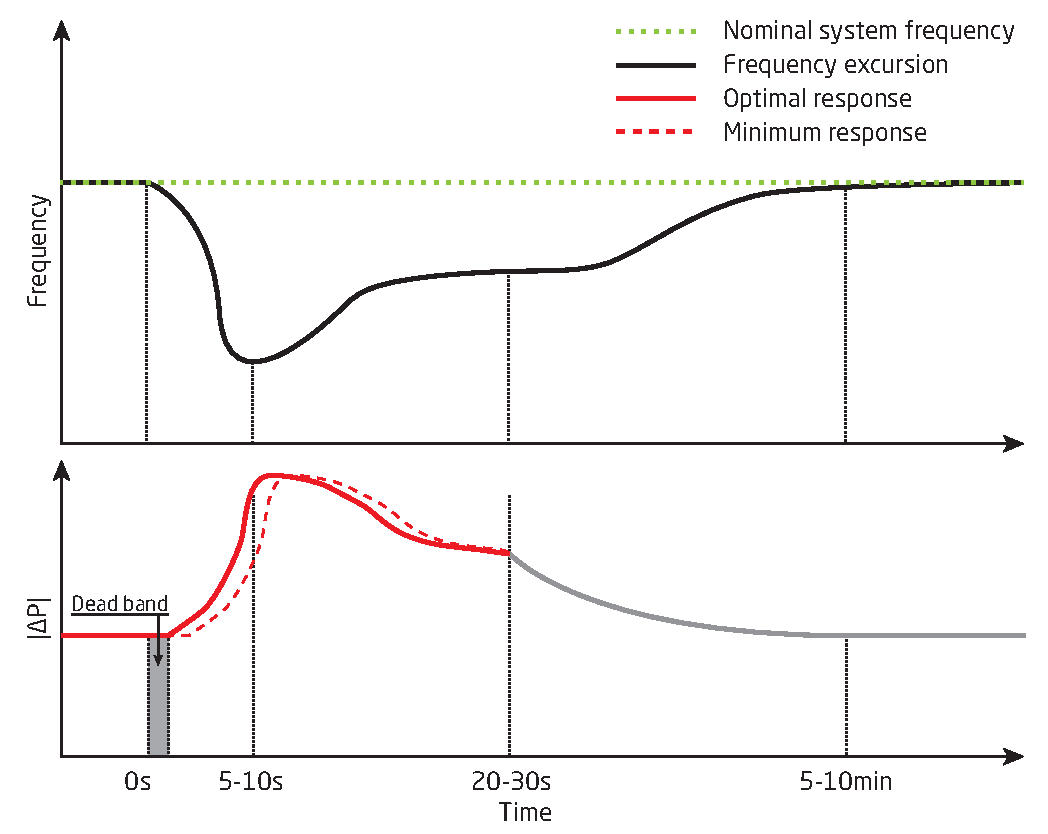
\includegraphics[width=1\columnwidth]{primary_frequency_control.pdf}
%\caption{Power response of a primary frequency control providing unit with perfect frequency following and with a droop of 4\%.}
%\label{fig:primarydroopresponse}
%\end{figure}
%
%Another way of formulating the optimal response is in terms of the rise time of the response (Figure~\ref{fig:primarytimeresponse})\cite{eto2010use}.
%\begin{figure}[ht!]
%\centering
%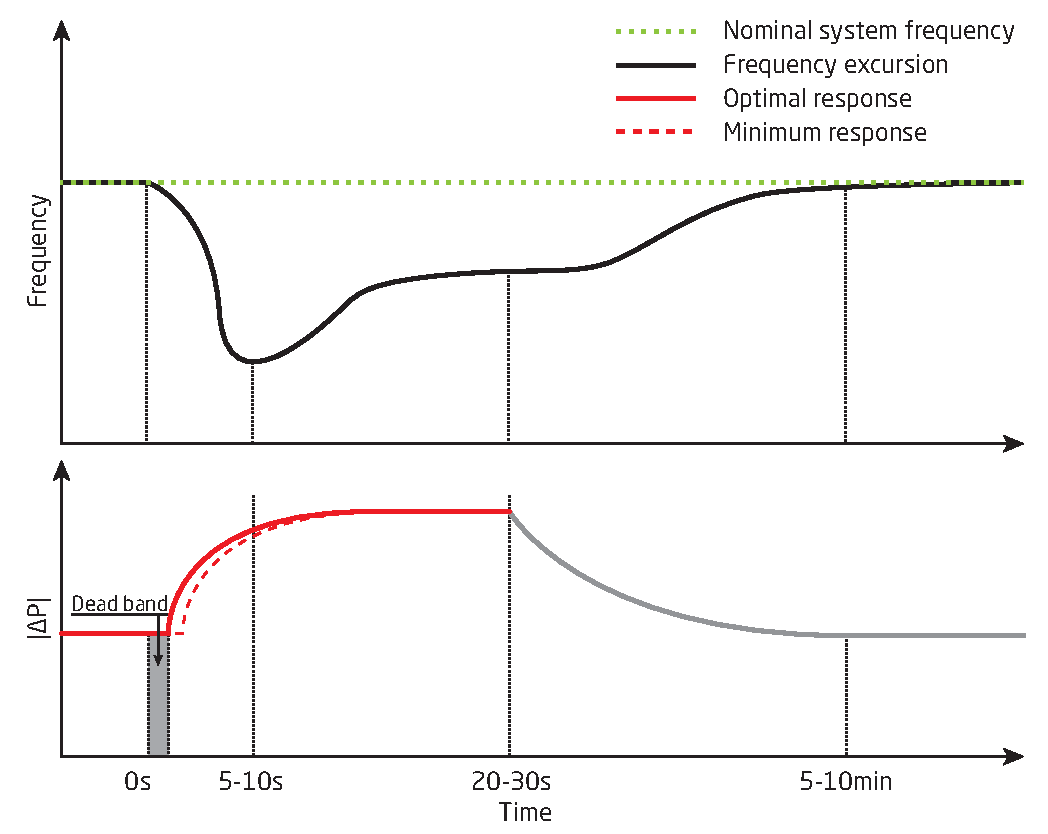
\includegraphics[width=1\columnwidth]{primary_frequency_control2.pdf}
%\caption{Power response of a primary frequency control providing unit when full delivery must be achieved within a time frame.}
%\label{fig:primarytimeresponse}
%\end{figure}
%
%For the secondary frequency control, the optimal response is formulated as a step function, or near step function because a response that is too steep could cause system instability. As in primary frequency control, the limits are defined by the allowable delay and a probabilistic term (Figure~\ref{fig:secondarytimeresponse}).
%\begin{figure}[ht!]
%\centering
%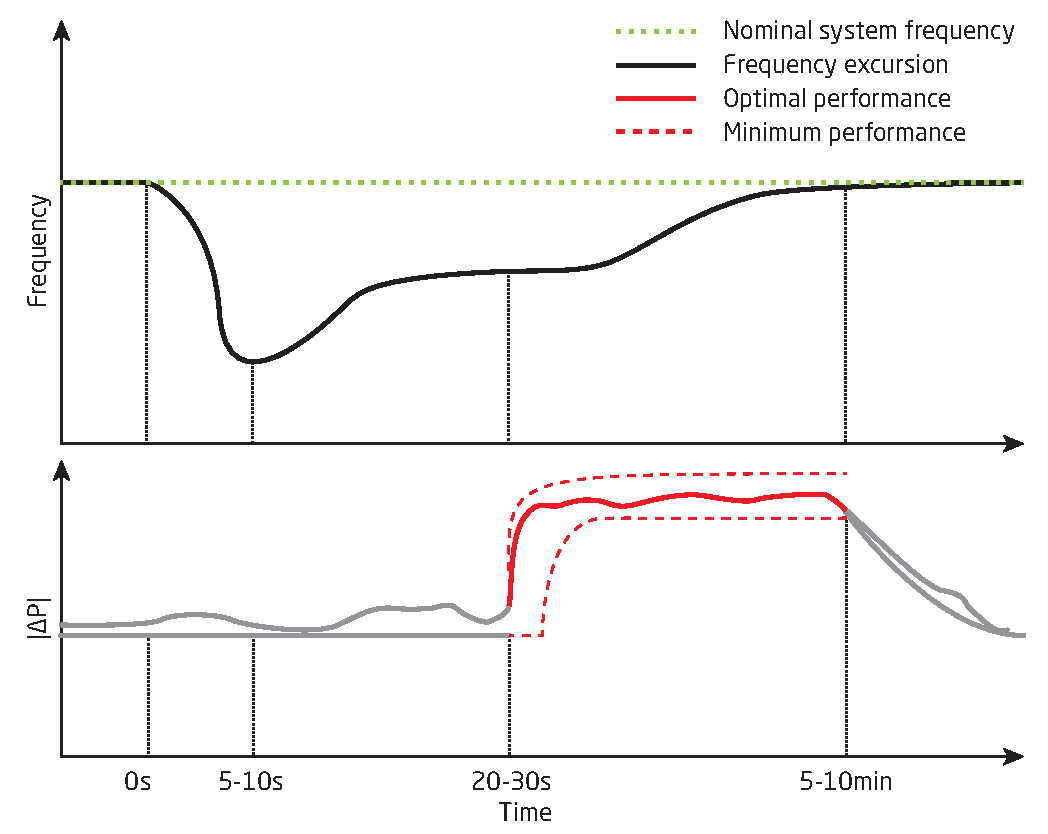
\includegraphics[width=1\columnwidth]{secondary_frequency_control2.pdf}
%\caption{Power response of a unit providing secondary frequency control indicating a time frame in which full delivery must be achieved.}
%\label{fig:secondarytimeresponse}
%\end{figure}
%We have identified three categories of requirements for ancillary services: performance requirements, unit specification requirements and market requirements.
%
%For primary frequency control the classification is the following:
%
%\emph{Performance requirements:} 
%\begin{itemize}
%\item Full availability
%\item Deployment end *
%\item Frequency characteristic
%\end{itemize}
%
%\emph{Unit specification requirements:}
%\begin{itemize}
%\item Droop of generator
%\item Compulsory adjustable droop
%\item Accuracy of frequency measurements
%\item controller insensitivity
%\item full deployment before a deviation of \emph{X} frequency
%\item Accuracy of SCADA measurements **
%\end{itemize}
%
%\emph{Market specification requirements:}
%\begin{itemize}
%\item Minimum reserve/bid size
%\item Contract \emph{X} time before delivery
%\item Bid symmetry
%\item Combined delivery
%\end{itemize}
%
%For secondary frequency control the classification is the following:
%
%\emph{Performance requirements:} 
%\begin{itemize}
%\item Deployment start
%\item Full availability
%\item Deployment end *
%\end{itemize}
%
%\emph{Unit specification requirements:}
%\begin{itemize}
%\item Control architecture
%\item Accuracy of frequency measurement
%\item Exchanges measurement
%\item Controller cycle time
%\item Controller type (P-term and I-term if applicable)
%\item K-factor for measuring ACE
%\item Accuracy of SCADA measurements **
%\end{itemize}
%
%\emph{Market specification requirements:}
%\begin{itemize}
%\item Minimum bid size
%\item Contract \emph{X} time before delivery
%\item Bid symmetry
%\item Combined delivery
%\item Bid duration
%\end{itemize}
%
%For tertiary frequency control the classification is the following:
%
%\emph{Performance requirements:}
%\begin{itemize}
%\item Deployment start
%\item Full availability
%\item Deployment end\textcolor{red}{(not sure on this one, since in many cases it is a rescheduling)}
%\end{itemize}
%
%\emph{Unit specification requirements:}
%\begin{itemize}
%\item Accuracy of SCADA measurements **
%\end{itemize}
%
%\emph{Market specification requirements:}
%\begin{itemize}
%\item Minimum bid size
%\item Contract \emph{X} time before delivery
%\item Bid symmetry
%\item Combined delivery
%\item Bid duration
%\end{itemize}

\section{Case Study}
\label{sec:ddrascasestudy}
%
\subsection{Case 1: Primary Frequency Control}
For example, for primary frequency control, which expects a step response from a nominal set-point to a new set-point based upon the frequency deviation, the TSO needs to establish two parameters:
\begin{itemize}
\item Optimal ramp time per bid atom
\item Optimal service duration
\end{itemize}

The optimal ramp time needs to be defined by the TSO, and will be derived from the inertia of the system. For example, the Danish TSO could determine that the optimal ramp time to be 0.001 s.

The optimal service duration depends solely on how fast it is able to activate secondary reserves. Again, in the Danish case 15 minutes is chosen to be the optimum.

Thus the performance value of units expecting to provide primary frequency control services can be characterised by:
\begin{align}
\kappa &= \alpha_1 \frac{\tau_{r,0}}{\max({\tau_{r,0},\tau_{r,a})}} + \alpha_2  \frac{\min(\tau_0,\tau_{a})}{\tau_{0}}\label{eq:kappa_primfreq}\\
\sum_{i} \alpha_i &= 1
\end{align}
where $\tau_{r,a}$ is the actual ramping time that the AS-providers can deliver, $\tau_{r,0}$ is the optimal ramping rate that the TSO would like to have. Similarly, $\tau_a$ is the endurance time that providers can deliver, and $\tau_{0}$ the the ideal endurance time the TSO would like. 
The TSO can assign a priority to any of the two variables by adjusting the weight factor $\alpha \in [0,1]$.

The formulation of equation~\eqref{eq:kappa_primfreq} has the property that a fast responding/short endurance service provider may be as valuable as a slow responding/long endurance service provider. 

\subsection{Case 2: Load Frequency Control}

E.g. for AGC/regulation/LFC:

1) The system requirements for the AS are: 
\kh{Esteban, what's the numbers again? cheers}
\begin{itemize}
\item Maximum ramp time for procurement volume $\tau_r$
\item Maximum activation time for 5\% procurement volume $\tau_{r5}$
\item Expected (minimum) duration of service $\tau_E$
\end{itemize}

2) \textbf{Tender:}
$P_{R,tot}$ total volume

Bid Parameters: 
$P_{R,a}$ - bid volume, $R_{a}$ - ramp rate, $\tau_a$ - duration 
\kh{i am not sure if we should formulate the limit as 'energy' or as 'duration', as the effects are quite different in case of partial activation --kai}


Other Service properties:

Performance parameter:
\begin{align}
\kappa &= \alpha_1 \frac{\min({R_{0},R_a})}{R_0} + \alpha_2  \frac{\min(\tau_0,\tau_{a})}{\tau_{0}}\label{eq:kappa2}\\
\sum_i\alpha_i &=1
\end{align}

3) 

\begin{figure}[htb!]
\centering
\includegraphics[width=1\columnwidth]{utility_ramp_endurance.png}
\caption{Caption it yourself!}
\label{fig:utrend}
\end{figure}
To be finished

\section{Discussion}
\label{sec:ddrasdiscussion}
%\section{Discussion}
Specific terminology has been introduced to describe the proposed method. This terminology can be mapped to that of the field of \emph{Design of Experiments}, e.g. \emph{definition of service requirements} maps to \emph{definition of inner-noise factor} and \emph{definition of test inputs} maps to \emph{definition of outer-noise factors}. Specifically, the method resembles \emph{fractional factorial methods for off-line quality control}, see e.g.\cite{oehlert2010first}. In the case study presented in Sec.~\ref{sec:casestudy}, the inner factor, or controllable variable, is kept at a single level, i.e. the same activation signal is sent to the aggregator for each run of the experiment. The two outer factors, or noise variables, were varied over a distribution dictated by the operational scenario, i.e. the availability of the portfolio was varied on seven levels and, likewise, the process noise in the house simulation models was varied on seven levels. An important contribution of this work is applying this kind of formal test procedures to the problem of aggregator validation. The field of Design of Experiments is broad, and a further revision on the topic may yield a better method proposals than the one proposed here.

In this paper we focus only on the two  uncertainty sources mentioned above, therefore the test for time responsiveness, i.e. delay in the communications systems between the aggregator and a DER is not considered. This means that the test design presented in the case study is a simplified version of what an actual aggregator validation test would require. Future research must identify the relevant variables that need to be tested under the relevant operation scenarios. 

In comparison with the traditional test method, this validation procedure must capture the capabilities of a much more complex system, and therefore relies in part on simulations. As presented in \cite{steinbrink2015challenges}, the error between the used models and reality must be quantified and taken into account for the final aggregator certification. Each block in the simulation must use validated models or software. This applies to the communication systems, the grid models and the DER models. The test architecture, e.g. the one presented in \cite{buscher2015towards}, which validates the aggregators must also be validated.

There are still several open issues that need to be investigated with regards to aggregator validation. For example, the definition of the operation scenarios was only briefly discussed, and heuristics must be developed in order to define scenarios that are effective when testing aggregators.

Aggregator validation must be an ongoing process, that should be carried out periodically or whenever the aggregator portfolio or architecture changes significantly. Furthermore, aggregators are expected to participate in different electricity markets. Due to these reasons, along with the complexity of designing appropriate simulations, we believe that the task of validating aggregators should not carried out by the system operators, but by an independent third party. 
To be finished
\section{Conclusion}
\label{sec:ddrasconclusion}
%\section{Conclusion}
This work presents an initial approach to establishing a method for designing aggregator validation tests. This method differs from the traditional generator certification tests in that it relies on a statistical approach. Specifically, it reinterprets the generator certification tests to aggregators by adapting concepts from statistical testing to the problem. The validation test must be carried out with the aid of simulations, so that the stochasticity of the real world disturbances affecting the aggregator can be taken into account. 

While several of the concepts that form the proposed validation procedure, e.g. software framework for aggregator tests and aggregator performance assessment, have been addressed before, this work describes how these concepts can be unified in order to do a systematic testing of aggregators.

The validation procedure was shown through a simplified case study on an existing aggregator design. While the example shows a fictive setup, it appropriately represents the procedure.

An important step for the development of the validation method is the implementation of a complete test architecture with validated component models. With such a simulation framework, with realistic communication and DER models, communication delays can be implemented in order to test aggregators for time responsiveness. 

We consider the work presented here an important element of enabling aggregators in the smart grid, thus enabling consumption to actively participate in the secure operation of the power system. This will help the integration of renewable energy sources into the power system.

To be finished
\section*{Acknowledgments}
We thank the following people for interview/feedback:
\begin{itemize}
	\item Scott Baker (PJM)
	\item Joe Eto (LBNL)
	\item Preben Nyeng, Peter Bruhn (Energinet.dk)
\end{itemize}
Parts of this work are supported by the Programme for Energy Technology Development and Demonstration (EUDP) and Innovation Fund Denmark through the iPower project.
%!TEX root = ../Thesis.tex
\chapter{Performance Assessment of Aggregation Control Services for Demand Response}\label{app:isgt2014}

\textbf{Authors:}\\
Daniel Esteban Morales Bondy\\
Giuseppe Tommaso Costanzo\\
Kai Heussen\\
Henrik W. Bindner

\noindent
\textbf{Published at:}\\
Innovative Smart Grid Technologies Conference Europe (ISGT-Europe), 2014 IEEE PES

\noindent
\textbf{Abstract:}\\
Aggregation algorithms that provide services to the grid via demand side management are moving from research ideas to the market. With the diversity of the technology delivering such services, it becomes essential to establish transparent performance standards from a service delivery perspective. This paper formulates performance measures and an index to evaluate in hindsight the quality of service delivery by an aggregator, both with respect to ancillary service and asset management service.


The index is based on requirements formulated in service contracts and provides an overall assessment of the quality of service provided by an aggregation control algorithm. By a detailed case study we present and an application of the index, comparing the performance of two different control architectures for demand side management delivering a distribution grid service.
\section{Introduction}

%Denmark has set as an objective that by 2050 the country should be independent of fossil fuels[source!, reformulate]. The integration of Renewable Energy Sources (RES), such as wind turbines and photovoltaic cells, and Distributed Energy Resources (DERs), such as EVs and heat pumps, will be integral to achieve this goal.

	The future increase in energy production from Renewable Energy Sources (RES) may lead to a power system where production is distributed, and where the Transmission System Operators (TSOs) require a larger amount of balancing services. At the same time, the increase in Distributed Energy Resources (DERs) brings new challenges to the Distribution System Operators (DSOs), which may need new kinds of ancillary services\cite{ipower2013development}. It is anticipated that DER owners will be able to provide services to the system operators via Demand Side Management (DSM). 

An Aggregator is a market player, or market role, whose business case is to manage DER units in its portfolio and use their inherent consumption flexibility to participate in the ancillary service markets, i.e. it controls units in order to perform DSM. A general classification of different aggregation methods is presented in \cite{kosek2013overview}, an example of direct control can be found in \cite{Biegel}, and an analysis and evaluation of indirect control architectures can be found in \cite{Heussen}.

Since the Aggregator has contractual obligations with customers and system operators, it is important that the control algorithm the Aggregator uses proves suitable for the task. From a service perspective, an aggregation algorithm is considered suitable if the performance, i.e. the quality of service (QoS), it delivers is within the contractual limits. The Aggregator must therefore control its DER portfolio in such a way that it fulfills the needs of both the DER owners and the System Operator.% The bounds of the QoS delimit the acceptable service provision, which is essential to the functioning of the power grid.

Little attention has been given to the problem of performance assessment of aggregator controllers seen from a service-delivery perspective. This paper approaches the problem by presenting two main ideas:
\begin{itemize}
	\item both ancillary services and DSM have minimum QoS requirements that need to be respected. In this work we propose a way of modeling the service requirements so that the quality of service delivery can be measured;
	\item a performance index suitable for evaluating the quality of aggregation control algorithms from point of view of the Aggregator.
\end{itemize}

The paper is organized as follows: Section \ref{sec:method} gives a general description of concepts relevant to the definition of the index, while the index itself is defined in Section \ref{sec:index}. A case study is presented in Section \ref{sec:case} and further research is discussed in Section \ref{sec:conclusion}.


\section{Background} \label{sec:method}

	\subsection{Ancillary Services} % (fold)
	\label{sub:ancillary}
	Ancillary services are acquired by TSOs in order to ensure the stability of the system and they can generally be divided into primary, secondary and tertiary ancillary services \cite{Rebours}. Each class of ancillary services has a different purpose in grid operation and works on different time scales.

	In the Danish system, producers, represented by a Balance Responsible Party (BRP), are allowed to bid into the ancillary-services market once they have been approved by the TSO. In order to be approved, the producers must prove that they are able to deliver the relevant services within the requirements defined in \cite{EnerginetAncillary,bondy2013}. Here, the TSO defines the bounds of error in service delivery, e.g. how much deviation with respect to a reference power schedule can be accepted before the service is considered non-delivered. In this work, the QoS measures the deviations from the contracted behavior.

	Furthermore, it is expected that new ancillary services will appear in the near future \cite{ipower2013development}. The two main problems that the DSO seeks to solve are congestion issues, i.e. overloading of cables or transformers, and voltage issues. Throughout this paper, the recurring example of an ancillary service is the \emph{PowerMax}, one of the new DSO services. This service is discussed further in Sec.\ref{sub:example}.
	% subsection ancillary_services (end)
	
	\subsection{Asset Management Service} % (fold)
	\label{sub:asset}
	Since the flexibility of individual DERs is too small to provide services to the system operators, an Aggregator pools the flexibility of the units, and presents their flexibility in the market as a single entity, see Fig.\ref{fig:systemarch}. Thus, the Aggregator is responsible for managing the DER units according to certain requirements defined by the owners, hereby providing an asset management service. This service must respect the primary function of the DER. 
	
	By changing the consumption behavior of DER units, the Aggregator performs Demand Side Management (DSM), providing ancillary services to the DSO or, through a BRP, the TSO. The Aggregator and the BRP could be the same entity, but if they are not, the Aggregator should not work against the balancing responsibilities of the BRP.  
	
	\begin{figure}[t]  % Find out how to send it to next column.
		\centering
		\includegraphics[width=0.7\textwidth]{isgt2014/system.eps}
		\caption{The setup of the power system with DSM. Note that the Aggregator can either be an independent entity or can be a role inside a BRP.}\label{fig:systemarch}
	\end{figure}
	
%	The objective of a DER is to satisfy the needs of its owner. The Aggregator provides the DER owners with an asset management service that ensures the QoS to customers is adequate. Providing services to the grid is only a secondary (and optional) function of the DER, which the Aggregator must take advantage of within the constraints of the primary function. 
	
%	The power consumption of DERs varies greatly depending on the daily routines of their owners and the meteorological conditions. Due to the varying load size, behavior and distributed nature of the DERs, the Aggregator must be able to evaluate if its control algorithms are capable of providing ancillary services and asset management satisfactorily.

	% subsection asset_management_service (end)
	
	\subsection{Control Performance Assessment}
	There is a field of theory on evaluation of controllers: Control Performance Assessment (CPA). Applications of this theory are found mostly in the process industry; for a thorough overview of its applications we refer to \cite{jelali2006overview,Green}. 

		Typically, CPA methods fall within two approaches. One approach, first introduced in \cite{Harris1989}, is to benchmark controller performance against a theoretical optimum, while taking the stochasticity of the system into account. The second approach is to benchmark against deterministic properties the closed-loop system must have, e.g. settling time and steady-state error \cite{Astrom}. In both cases, the index is usually scaled such that:
\begin{equation}
	\zeta = \frac{J_{opt}}{J_{act}},\label{eq:astrom}
\end{equation}
where $J_{opt}$ is the theoretical optimal (minimum) value of the performance criterion \emph{J} (which is usually impossible to achieve in reality), and $J_{act}$ is the actual measured value of the criterion. Since $J_{opt}<J_{act}$, then $\zeta \in [0,1]$. 
		%Given that the requirements of service delivery are easily translated into time-domain deterministic measures, this work presents a deterministic approach. Using the concepts presented in this section, the performance index is defined in the next section.
%In the following, we propose the application of CPA concepts to DSM.

		According to \cite{Green}, performance criteria used to evaluate a controller usually fall within three categories: Quality, Reliability, and Energy. Quality and reliability are concepts that can be directly related to ancillary service provision. The interpretation of energy-related criteria may be suitable for asset-management purposes but is considered out of scope in this work.% The quality of the control performance is measured by the QoS it provides, both towards the system operators and towards its customers. Reliability is measured as how many times the controller provides a QoS outside the specified limits.

\section{DSM Performance Assessment} % (fold)
\label{sec:index}
We identify four requirements for performance assessment of DSM:
\begin{itemize}
	\item[R1] Provide a \emph{quality} measure normalized to the contractual requirements (bounds) of a service. By normalizing the quality measure to the bounds, the \emph{QoS} value for both ancillary services and asset-management services will have comparable dimensions.
	\item[R2] The measure should be normalized with respect to time.
	\item[R3] Provide a \emph{reliability} measure in relation to service non-delivery.
	\item[R4] Each service must have a separate, individually verifiable, measure. For example, to evaluate service delivery w.r.t. ancillary-service delivery, the asset-management quality is irrelevant.
\end{itemize}

To satisfy these requirements, we propose a performance index quantifying the quality of ancillary services and asset-management services, and a non-delivery counter (NDC) which increases every time the QoS is out of bounds. Normalization is based on a scaling factor modeled after the contractual limits of the respective service. The limits are defined via a contract with the entity requesting the service. Thus, the performance index is specifically designed to evaluate how well the service provision conforms to the contractual boundaries.
	%The formulation of a performance index transforms the service requirements of the Aggregator into a single computable quality measure. %The index presented here is defined for post-simulation analysis, and represents the performance of the control algorithm over the whole time horizon. 
	\subsection{Definition of the performance index}
	In previous sections we have defined the concept of QoS as a deviation, $e(t)$, from a contracted behavior. Since there is a contractual limit on the allowed deviation, the error is normed to be a percentage of this limit such that:
	\begin{equation}
		QoS_{s}(t)=|e(t)|C_{s}(t); \quad  QoS_{s}(t)\in [0,1]
	\end{equation}
	where \emph{s} is either \emph{AS} for ancillary service or \emph{AMS} for asset-management service, and $C_s(t)$ is the corresponding normalization factor derived from the service model. When $QoS_{AS}(t) \geq 1$, the measure for reliability NDC is increased. %For the ancillary services this is simply expressed as $QoS_{AS}(t) = e(t)_{AS}$ while the expression for the asset management service is $QoS_{AM}(t) =\sum_{k=1}^M e(t)_{AM}$.

	Using the square root of the Integral Square Error index (i.e. the 2-norm, as defined in e.g. \cite{Skogestad}), the following performance criterion is defined for service delivery seen from the Aggregator perspective:
	\begin{equation}
		%\text{J}=\sqrt{\int_{0}^{N}\left( \sum_{k=1}^M |e(t)_{AM,k}C_{AM}|^{2}+|e(t)_{AS}C_{AS}|^{2}\right)dt} 
		{J}(N)=\sqrt{\int_{0}^{N}\left( \sum_{k=1}^M {QoS}_{AMS,k}(t)^{2}+{QoS}_{AS}(t)^{2}\right)dt} 
	\end{equation}
where ${QoS}_{AM,k}(t)$ and ${QoS}_{AS}(t)$ are the time-dependent measures of service quality for the asset-management service and the ancillary service, respectively. The units controlled by the Aggregator are denoted by the index \emph{k}, the unit portfolio is of size \emph{M}, and \emph{N} is the time horizon over which the services are provided. %Finally, $Q_D$ and $Q_U$ are scaling factors that convert the errors into percentages so that $e(t)_D$ and $e(t)_U$ are comparable. 
While the index~\eqref{eq:astrom} benchmarks the actual performance criterion against a theoretical minimum, we benchmark it against the worst case scenario $J_{max}$, such that the performance index is given by:
	\begin{equation} 
		\eta = \frac{J_{act}(N)}{J_{max}(N)}\label{eq:eta}
	\end{equation}
	where $\eta \in [0,1)$ for a valid service delivery and for which values close to zero represent good performance of service delivery. If $\eta \geq 1$ the Aggregator does not perform according to its service contract.
		
		Normalization with respect to time is achieved when benchmarking against $J_{max}(N)$, since $J_{max}(N)$ is estimated by integrating over the service delivery period. Contrary to index \eqref{eq:astrom}, which gives an intuition of how close performance is to the optimum, index \eqref{eq:eta} gives an intuition of how far performance is from the worst case scenario. The index is designed this way because the theoretical optimum of service delivery is $J_{opt}=0$, i.e. no error in service delivery.
	%It must be noted that the performance criterion only measures the permissible error defined in the contract of the service (the service quality), and service non-delivery (the service reliability) is measured separately. Therefore, whenever the algorithm performs outside the established limits, then $J(t)_{act}=J(t)_{max}$ and a non-delivery counter is increased.
	\subsection{Calculating the index}\label{sub:modelcalc}
	Having defined what the performance index measures, we will proceed with establishing how to obtain the required values to estimate the index. Calculating the performance index requires the following steps:
	% the maximum permissible error ($J(t)_{max}$) of the service requires two steps:
		\begin{enumerate}
		\item Identify and model the service requirements and errors in service provision, giving the scaling factor $C(t)_s$.
			\item Estimate $J_{act}(N)$.
			\item Calculate \emph{J(N)} for operation on the requirement boundaries ($J_{max}(N)$).
			\item Calculate $\eta$ by benchmarking $J_{act}(N)$ with $J_{max}(N)$.
		\end{enumerate}	
		
	For the first step, the service requirements must be defined and translated into measurable errors. For some services, the error can be stated as a tracking error, e.g. $e=y_{ref}-y_{meas}$. In other cases, service requirements are defined by operation within bands, which may lead to an error defined as:
	\begin{equation}
	e(x)= \left\{ \begin{array}{l l}
	x_{min} - x & \quad \text{ if } x \leq x_{min}\\
	0 & \quad \text{ if } x_{min} \leq x \leq x_{max}\\
	x - x_{max} & \quad \text{ if } x \geq x_{max}
	\end{array} \right.
	\end{equation}
	This step is a service-specific problem and is non trivial.

	The second step requires computing $J_{act}(N)$ using measurement data from the unit portfolio. This can be a challenge for evaluation in field deployment. In this paper it is assumed that the measurement data is available, either through a DSO or a third-party metering company.	
	
		%The actual performance of the aggregation algorithm can be found through two different methods:
%\begin{itemize}
	%\item On-line monitoring -- This method brings the added benefit of being able to use the index for performance monitoring and diagnosis at runtime, but the downside of being communication intensive.  
	%\item Post-delivery analysis -- This method is less communication intensive, but does not permit to take remedial actions at run time if a aggregation controller is not working as expected.
%\end{itemize}
%	Usually services have some acceptable error (see Sec.~\ref{sub:ancillary}) which can be interpreted as the hard boundaries for the service delivery.
	The third step requires the calculation of \emph{J(N)} along the contractual boundaries for service delivery, in this way, the maximum allowed error is found for the service. The boundaries are based on the service models presented in the first step. By adding the maximum permissible error for all services, $J_{max}(N)$ is obtained. 
	%Normalizing the performance measure with the $J_{max}$ gives an intuitive value of the performance of the control algorithm.
	The following subsection present an example of how to determine $J_{max}(N)$.

	\subsection{An example: DSO Service PowerMax}\label{sub:example}
	For demonstration purposes, in this section $J_{max}(N)$ for the PowerMax service is calculated. 
	Typically, the service will be contracted several months ahead of the actual delivery. The activation schedule (On and Off triggers), the maximum power cap ($P_M$), the maximum duration of the service per activation ($T_M$), and the quality of service (\emph{QoS}) are defined when contracting the service. The contract is valid for a period of several months, where the Aggregator is obliged to follow the established schedule.

	The limits specified for the QoS\cite{ipower2013development} of the PowerMax service are presented here: 
	\begin{itemize}
		\item Deviation from On trigger: $\pm$ 15 min. per day
		\item Deviation in size of service (dependent on $P_M$): Max. $\pm 5\% P_M$  
		\item Acceptable no. of unsatisfactory activations(non-delivery): $\text{NDC} = 4$
	\end{itemize}

A graphical representation of these service requirements is depicted in Fig.~\ref{fig:servicereq}. It is clear that the maximum acceptable error in service delivery is the shaded area. Note that the limit for non-delivery of service during the first 15 minutes of activation is dotted due to the fact that non-delivery is not counted during this period. The specifications for counting unsatisfactory activations are not clarified in \cite{ipower2013development}, so it is assumed that breaking the QoS limits on one sampling period counts as one non-delivery. In the case where the service is not respected in three consecutive (or non-consecutive) sampling periods, $\text{NDC}=3$.

For example, in the case where  $P_M = 5\,kW$, $T_M=4\, h$ and the power is measured once an hour, $J_{max}(N) = 2$, as it represents the square root of the square of the maximum (when $J_{act}(N)=1$) permissible error over 4 hours.
\begin{figure}[t]  % Find out how to send it to next column.
	\centering
	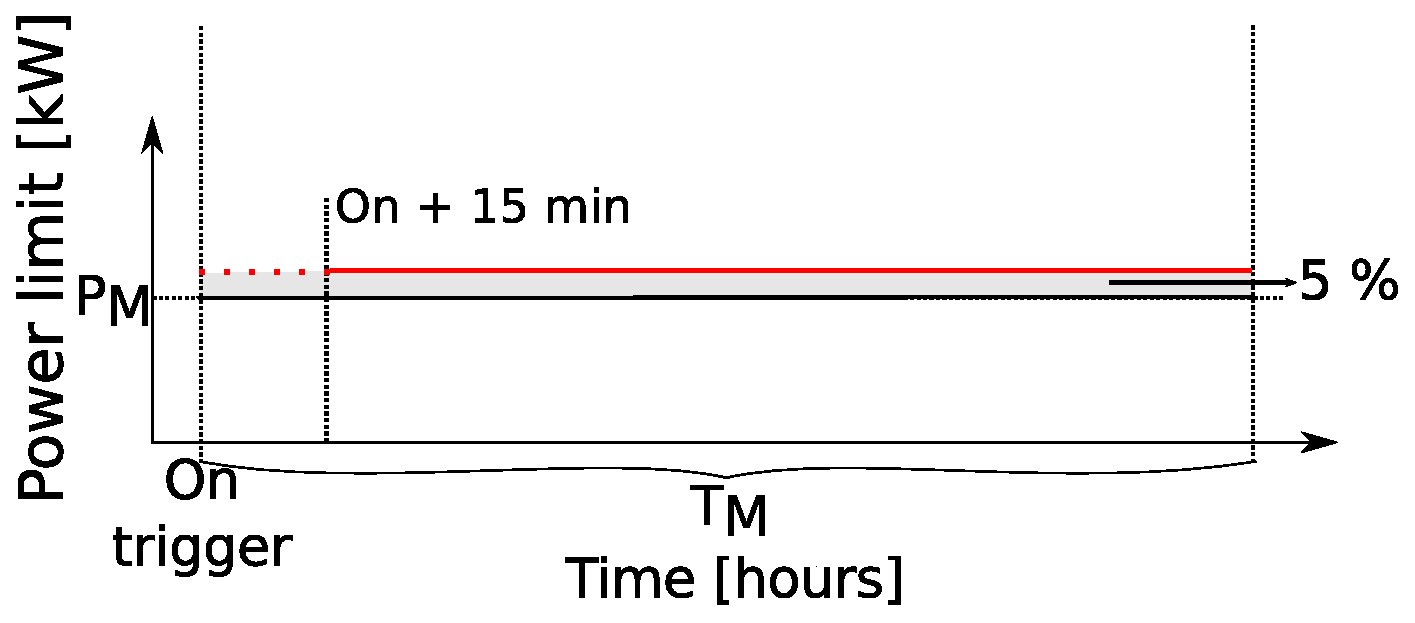
\includegraphics[width=2.5in]{isgt2014/drawing3.eps}
	\caption{The PowerMax service requirements, where the red line represents the boundaries for the permissible error, and the shaded area represents the error in service delivery, which is within the limits established in the QoS. }\label{fig:servicereq}
\end{figure}

	
% section the_performance_index (end)

\section{Case Study}
\label{sec:case}
This case study presents the aggregation of multiple flexible DERs via coordinated operation: 75 DERs installed in a suburban residential area, which are all connected to the same feeder leading to a 10/0.4 kV transformer. The transformer is rated to a maximum power flow of 200 kVA, which is sufficient under the current load circumstances, but will be a constraint in the future.

This case study addresses a scenario with high electric-vehicle (EV) penetration, low photo-voltaic (PV) penetration and electric space heating in all households. Furthermore all DERs connected to the same LV feeder offer their flexibility to the same Aggregator. Then, the proposed performance index for service provision is evaluated for two different aggregation control algorithms: Centralized soft Model Predictive Control (C-MPC) and Distributed soft Model Predictive Control (D-MPC).

\subsection{The reference case: without units coordination}
In this section we make a scenario hypothesis for year 2050 regarding PV and EV penetration in a distribution feeder in a rural area and present simulation results. The following units are connected to the LV transformer:
\begin{itemize}
\item 40 buildings with electric climate control: resistive space heating with maximum load of 10 kW and air conditioning with a maximum load of 5 kW.
\item 20 large EVs, with a battery size of 25 kWh, 11 kW.
\item 10 small EVs, with a battery size of 14 kWh, 3.3 kW.
\item 5 PV (polycrystalline) installations of 6 kW rated power each.
%\item 5 Li-On support batteries for local energy storage: 10 kWh, 2 kW each (95\% round trip efficiency). 
\end{itemize} 

The PV installations provide forecasts of the production for one day ahead. To simulate uncertainty in the forecasts, Gaussian noise has been added to real data of PV production according to:
\begin{equation}
	{P_{PV-F,t}} = {P_{PV-T,t}} + {v_t},\quad {v_t} \sim N\left( {0,\alpha  \sqrt {{P_{PV-T,t}}} } \right)\label{eq:pvprod}
\end{equation}
where $P_{PV-F,t}$ is the forecasted PV power production at time $t$, and $P_{PV-T,t}$ is the actual power production at time $t$ (from historical data). The term $\alpha$ is an uncertainty factor, which defines the variance of the noise as a percentage of the actual PV production, e.g. $\alpha = 0.1$ corresponds to a $10\%$ forecast error. Uncertainty in solar radiation and ambient temperature are modeled in the same way. The actual power production time-series used in this case covers the same days as \cite{costanzo2013coordination}.

The load related to households is divided into climate control (flexible load) and everything else (non-flexible load). The building climate control is operated on MPC basis for minimum deviation from the temperature set point. Regarding the non flexible household loads, a five-day (one-hour-sampled) profile of the non-flexible load of 40 households is depicted in Fig.~\ref{fig:nonflexible}.

\begin{figure}[t]  
	\centering
	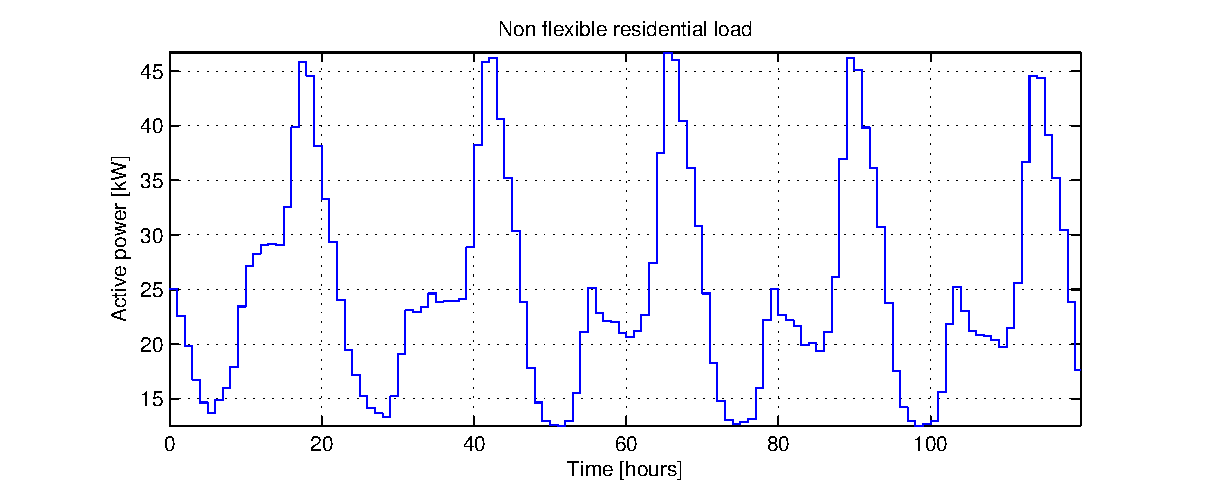
\includegraphics[width=\textwidth]{isgt2014/nonflexload.eps}
	\caption{The non-flexible load of the households under the transformer. The sample is statistically representative of Danish households.}\label{fig:nonflexible}
\end{figure}

The EVs leave the charging station at a uniform randomly distributed time between 6:00  and 8:00, and are plugged again at a uniform, randomly distributed time between 16:00 and 18:00. The EVs operate on dumb charging, i.e. they try to fully charge as soon as they are connected to the grid.  %The energy price is the same for all the units within the same cluster.
By running a simulation of the described scenario without units coordination, the results shown in Fig.~\ref{fig:referencecase} are obtained.

\begin{figure}[t]  
	\centering
	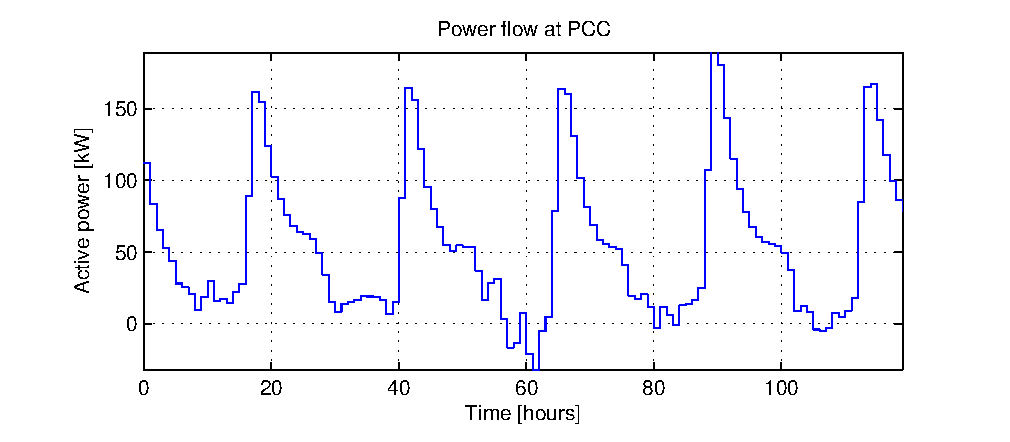
\includegraphics[width=\textwidth]{isgt2014/referencecase.eps}
	\caption{Aggregated power flow at the point of common coupling for the reference case units without coordination: Demand Response based on day-ahead energy price.}\label{fig:referencecase}
\end{figure}

EVs operating on dumb charging can cause peak consumption up to 190 kW at the point of common coupling (PCC). Given that the transformer capacity is 200 kW and it is customary to reserve 30\% of the transformer capacity for emergency operations \cite{Engel}, the DSO aims at keeping the load below 140 kW and limiting the inverse power flow at the substation. Thus, the DSO can sign a contract for PowerMax service (see Sec.~\ref{sub:example}) with an Aggregator which, at any time, operates Demand Response via Direct Load Control (DLC)~\cite{kosek2013overview} in order to limit the power flow at the transformer. The maximum capacity available at the transformer is therefore 140 kW for direct power flow and -10 kW for inverse power flow.

The rest of this section presents the C-MPC and D-MPC formulations. For the formulation of the mathematical models we refer to~\cite{6345063} for the battery model and to~\cite{Bacher20111511} for the building space heating model (modified, as proposed in~\cite{costanzo2013coordination}). For the modeling of the services, we apply the method described in Sec.\ref{sub:modelcalc}. A discussion on the simulation results concludes this section.
\subsection{The Centralized Model Predictive Control scheme}
\begin{figure}[t]  
	\centering
	\subfloat[The setup of the Centralized MPC scheme.]{\includegraphics[width=1.0\textwidth]{isgt2014/centralized.eps}\label{fig:centralized}}
\\
\subfloat[The setup of the DMPC scheme as seen in \cite{costanzo2013coordination}.]{\includegraphics[width=1.0\textwidth]{isgt2014/blackboard.eps}%
\label{fig:blackboard}}
\caption{The setup of the two Aggregation algorithms to be compared.}\label{fig:systemsetup}
\end{figure}
In this scheme the Aggregator contains the control algorithm to centrally manage all the units in its portfolio (Fig.~\ref{fig:systemsetup}(a)). Since the Aggregator optimizes its portfolio's consumption through MPC, it has detailed knowledge of the state and dynamics underneath.
The units portfolio is the same as of the reference case. The C-MPC control problem is formulated as quadratic optimization with soft constraints (as seen in e.g. \cite{prasath2009a}):
{%\footnotesize
{\begin{subequations}\label{Eq: building_MPC}
\begin{align}
& \min\limits_{u_t,\vartheta_t} \; {J} = \sum\limits_{t = 1}^N {\left[ {\left\| {y_{t} - r_t} \right\|_Q^2} + {\rho}\vartheta_t + \psi \gamma_t \right]} \label{Eq: building_MPC_objective}\\
& subject \; to: \nonumber \\
& x_{t + 1} = Ax_t + B u_t + Ed_t\label{Eq: building_MPC_constraint1}\\
& y_t = {C}x_t +Du_t \label{Eq: building_MPC_constraint2}\\
& u_{\min ,t} \le u_t \le u_{\max ,t} \label{Eq: building_MPC_constraint3}\\
& y_{\min ,t} - \gamma_t \le y_{t} \le y_{\max ,t} + \gamma_t \label{Eq: building_MPC_constraint4}\\
& {PCC_{\min ,t}} - \vartheta _t \le u_t \le {PCC_{\max ,t}} + \vartheta _t \label{Eq: building_MPC_constraint5}\\
& \vartheta_t,\gamma_t \ge 0 \label{Eq: building_MPC_constraint6}
%& \gamma_t \ge 0 \label{Eq: building_MPC_constraint7}
\end{align}
\end{subequations}}}
where $r_t$ and $y_t$ are the output reference and system outputs (internal house temperature and battery state of charge) respectively over the prediction horizon $t=1..N$, $\psi$ is the weight for output soft constraints, with $\gamma$ being the corresponding slack variable, and $\rho$ penalizes the \emph{power over max} defined in Eq.~\ref{Eq: building_MPC_constraint5}. Since this MPC controller is centralized, the state space system matrices in Eq.~\eqref{Eq: building_MPC_constraint1} and Eq.~\eqref{Eq: building_MPC_constraint2} are formed by block diagonal-adding each of the systems' respective matrices. With the set of units $\mathcal{S}=\{1..N\}$, it follows:
%
{ \begin{equation}
\begin{array}{l}
x = \left[ {\begin{array}{*{20}{c}}
{{x_1}}\\
{{x_j}}
\end{array}} \right],u = \left[ {\begin{array}{*{20}{c}}
{{u_1}}\\
{{u_j}}
\end{array}} \right],d = \left[ {\begin{array}{*{20}{c}}
{{d_1}}\\
{{d_j}}
\end{array}} \right],y = \left[ {\begin{array}{*{20}{c}}
{{y_1}}\\
{{y_j}}
\end{array}} \right]\\
\\
A = \left[ {\begin{array}{*{20}{c}}
{{A_1}}&0\\
0&{{A_j}}
\end{array}} \right],\quad B = \left[ {\begin{array}{*{20}{c}}
{{B_1}}&0\\
0&{{B_j}}
\end{array}} \right]\\
\\
C = \left[ {\begin{array}{*{20}{c}}
{{C_1}}&0\\
0&{{C_j}}
\end{array}} \right],\quad D = \left[ {\begin{array}{*{20}{c}}
{{D_1}}&0\\
0&{{D_j}}
\end{array}} \right]\\
\\
E = \left[ {\begin{array}{*{20}{c}}
{{E_1}}&0\\
0&{{E_j}}
\end{array}} \right],\quad \vartheta  = \left[ {\begin{array}{*{20}{c}}
{{\vartheta _1}}\\
{{\vartheta _j}}
\end{array}} \right],\gamma  = \left[ {\begin{array}{*{20}{c}}
{{\gamma _1}}\\
{{\gamma _j}}
\end{array}} \right]
\end{array}
\end{equation}}
%\normalsize
where the index $j \in \mathcal{S}$ and the system in Eq.~\eqref{Eq: building_MPC_constraint1} and Eq.~\eqref{Eq: building_MPC_constraint2} is extended with all the units belonging to the set $\mathcal{S}$.
\subsection{The Distributed Model Predictive Control scheme}
%The computational effort for solving centralized MPC problems generally grows at a super-linear rate with the number of state variables involved. The exact order is problem-specific and depends on the coupling between the state variables as well as the chosen solving method. Decomposing the C-MPC problem into smaller MPC sub-problems that can be solved independently and locally at the unit level helps in solving the curse of dimensionality. Convergence towards the overall goal is then achieved through a blackboard coordination mechanism, which ensures data exchange between the individual solvers.
In the D-MPC formulation, units within the same cluster retrieve the power plans of the other units, compute their own plan (over a prediction horizon) accordingly and publish it on a blackboard. Note that in this case study, in contrast to what has been proposed in~\cite{costanzo2013coordination}, the unit controllers have soft constraints on the outputs (temperature for buildings and State of Charge (SOC) for batteries and EVs). In this algorithm, as soon as the units publish their consumption plan, the available power at the PCC decreases in such a way that the subsequent units communicating with the blackboard tend to adjust their plan accordingly. After a negotiation period the units are entitled to operate according to the power plan that has been published in the blackboard for the next time frame. Figure~\ref{fig:systemsetup}(b) shows the configuration for the D-MPC. This is an example of transactional control \cite{kosek2013overview}, where the unit power consumption is negotiated.
\subsection{Comparison and discussion of results} \label{sub:comparison}
Certain assumptions have been made with regards to controllers:

%\begin{itemize}
The EVs are preferably kept operating in the range $SOC = [0.2,0.9]$ due to battery life concerns\cite{6345063}, although it is possible to operate in $SOC=[0.0,1.0]$.
The comfort band for the households lies in the band $T_{ref}=22{}^{\circ} C \pm 1{}^{\circ} C $. The concept of non-delivery is not used in the asset-management services, but the absolute boundaries for user-comfort bands lie on $T_{ref}=22{}^{\circ} C \pm 1.5{}^{\circ} C $.

The required PowerMax service is of $P_M = 90kW $ each day in the periods of 16:30 to 20:30.
The time sampling of the simulation is of 15 minutes and the power plans are computed for a horizon of 23 hours (i.e. the MPC prediction horizon).
%\item The EVs are not available during the day, when they are used for transport, and in these periods the MPC for the EV is inactive.
The EVs are not capable of providing Vehicle-to-Grid (V2G) services, i.e. EVs only charge.

%\end{itemize}
These assumptions lead to the results presented Figs.~\ref{fig:dmpcsimres}-\ref{fig:pccsimres} and Tables \ref{tab:comparison}-\ref{tab:days}.
The following conclusions can be made:

1) from Figs.~\ref{fig:dmpcsimres} and \ref{fig:cmpcsimres} it can be seen that both controllers are quite good at staying within the QoS limits of the DSO and EV owners, which can be seen in the fact that none of the controllers have non-delivery and $\eta$ is small. It is clear that the value of $\eta$ comes from the behavior of the household heating, where the C-MPC delivers a better quality service to end users than the D-MPC, although it might not be obvious from the figures. % Also, from Fig.~\ref{fig:pccsimres}, it is clear that the PowerMax service is delivered at all times.

2) controller performance is sensitive to prediction uncertainties, as can be seen in the varying values of $\eta$ depending on the uncertainty $\alpha$ (see Eq.~\eqref{eq:pvprod}), which is shown in Table~\ref{tab:comparison}.
	%\item By changing some of the different weights on the controllers, e.g. prioritizing the upwards service versus the downwards service, leads to different results it $\eta$ (this is not shown in the figures).

3) in terms of service provision, the C-MPC outperforms the D-MPC. This arises from the fact that the C-MPC has absolute control of all units and determines a global optimum.

4) due to the behavior difference between the local EV controllers in the D-MPC scheme, and the behavior of the C-MPC, the power consumption of the EV is very different (compare Fig.~\ref{fig:dmpcsimres}(b) and Fig.~\ref{fig:cmpcsimres}(b)). This also leads to a vast difference in the power flow at PCC (see Fig.~\ref{fig:pccsimres}).

5) from the values in Table~\ref{tab:days}, it can be seen that the values of $\eta$ are in the same order of magnitude when simulations are done for varying numbers of days. This is caused by the normalization of $J_{act}(N)$ over time (reflected in $J_{max}(N)$). This means $\eta$ evaluates the aggregation algorithm taking service provision time into account, and gives an overall assessment of the algorithm, dependent on the length of time the Aggregator must sustain the service provision. %An error in provision of a specific size will have less impact on $\eta$ if the service time is long. This makes sense since an error  

\begin{figure}[!t]
\centering
\subfloat[Households temperatures]{\includegraphics[width=1.0\textwidth]{isgt2014/DMPCalpha01/building2.eps}%
\label{fig:dmpchouse}}
\\
\subfloat[EV State of Charge]{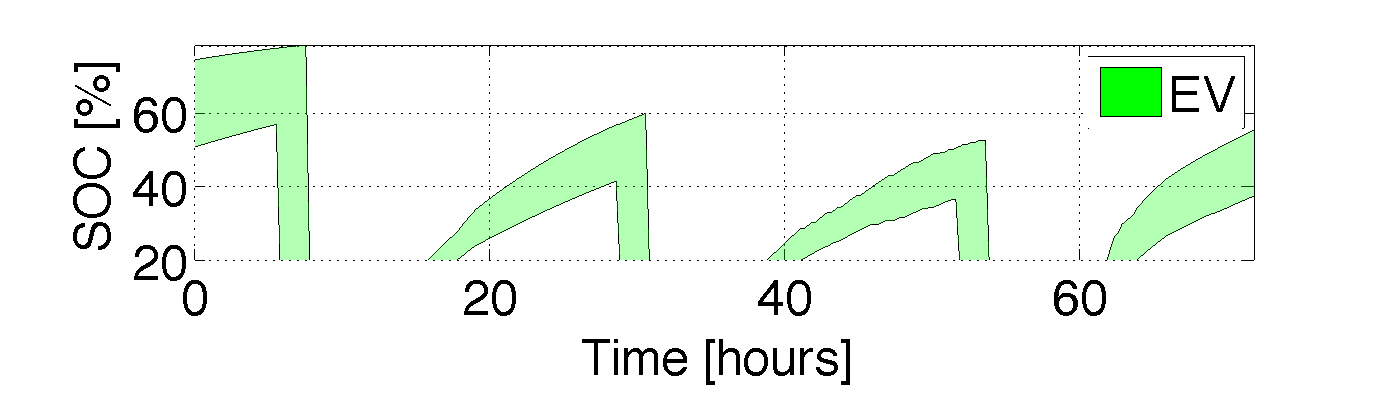
\includegraphics[width=1.0\textwidth]{isgt2014/DMPCalpha01/EVs.eps}%
\label{fig:dmpcev}}
\caption{Simulation results for the D-MPC with $\alpha=0.1$}
\label{fig:dmpcsimres}
\end{figure}

\begin{figure}[!t]
\centering
\subfloat[Households temperatures]{\includegraphics[width=1.0\textwidth]{isgt2014/CMPCalpha01/buildings.eps}%
\label{fig:cmpchouse}}
\\
\subfloat[EV State of Charge]{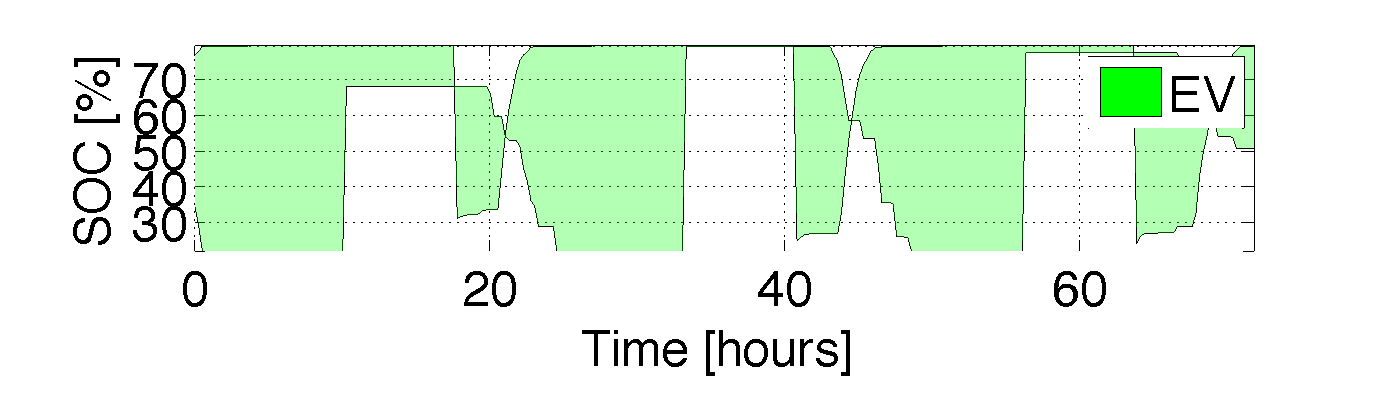
\includegraphics[width=1.0\textwidth]{isgt2014/CMPCalpha01/EVs.eps}%
\label{fig:cmpcev}}
\centering
\caption{Simulation results for the C-MPC with $\alpha=0.1$}
\label{fig:cmpcsimres}
\end{figure}

\begin{figure}[!t]
\centerline{\subfloat[Total power load for C-MPC]{\includegraphics[width=0.5\textwidth]{isgt2014/CMPCalpha01/PCC.eps}%
\label{cmpcpcc}}
\subfloat[Total power load for D-MPC]{\includegraphics[width=0.5\textwidth]{isgt2014/DMPCalpha01/PCC.eps}%
\label{dmpcpcc}}}
\centering
\caption{Power load at Point of Common Coupling for the controllable and non-controllable loads}
\label{fig:pccsimres}
\end{figure}

% increase table row spacing, adjust to taste
%\renewcommand{\arraystretch}{2.3}
%if using array.sty, it might be a good idea to tweak the value of
% \extrarowheight as needed to properly center the text within the cells
\begin{table}
\caption{Results of three-day simulation}\label{tab:comparison}
\centering
% Some packages, such as MDW tools, offer better commands for making tables
% than the plain LaTeX2e tabular which is used here.
\begin{tabular}{c|c c c c}
\hline
&\multicolumn{2}{c}{D-MPC} & \multicolumn{2}{c}{C-MPC} \\
\hline
$\alpha$ & 0.1 &0.2&0.1&0.2\\
NDC&0 &0 &0 &0\\
$\eta$&0.0075 &0.0160&0.0054&0.0153\\
\hline
\end{tabular}
\end{table}

\begin{table}
	\caption{D-MPC Performance over different simulation lengths}\label{tab:days}
	\centering
\begin{tabular}{c|c c c c c}
\hline
Days simulated & 1 & 2 & 3 & 4 & 5 \\
$\eta$ &0.0013&0.0018 &0.0082&0.0052&0.0062\\
\hline
\end{tabular}
\end{table}

	\section{Conclusion and Outlook}
	\label{sec:conclusion}
	Drawing inspiration from the field of Control Performance Assessment, this study proposes a performance index for the evaluation of control services for DER aggregation. The index is useful for the systematic evaluation of the adequacy of different control architectures providing ancillary services.
It was shown how the index is computed, and a case study was presented in which two different control algorithms were evaluated. The results were presented and discussed, showing that the C-MPC in this case is capable of providing a better QoS.
%Evaluation of aggregation algorithms is expected to be an important part of validation of Aggregators providing DSM. 
%	 As modelled in this paper, the index only gives a general idea of the performance of the control algorithm, but future work could include a method for differentiating the sources of high error.
	In order to do a successful evaluation of an aggregation algorithm, it is important that the QoS specifications of the future ancillary services are well defined. This is a challenge in itself since many of the ancillary services assume a production baseline, which is easy to establish in traditional generators, but proves to be difficult for small households (see e.g. \cite{Borenstein}). Research effort should be put into redefining ancillary-service requirements to suit DSM, taking into account the probabilistic nature of managing a large number of units.

 The evaluation of aggregation control algorithms is an important part of a general validation framework for Aggregators. Future work will include further development of this Aggregator validation framework, where controllers can be tested under different grid and communication network topologies, as well as a diverse set of fault scenarios.

\section*{Acknowledgment}

The authors acknowledge the financial support of iPower (www.ipower-net.dk).
The authors thank Shi You from DTU Elektro for providing data for the non-controllable loads.



%!TEX root = ../Thesis.tex
\chapter{Method for Ancillary Service Modeling and Performance Assessment}
\label{app:tsg}

\textbf{Authors:}\\
Daniel Esteban Morales Bondy\\
Anders Thavlov\\
Janus Bundsgaard Mosb{\ae}k Tougaard\\
Kai Heussen

\noindent
\textbf{Submitted to:}\\
IEEE Transactions on Smart Grid

\noindent
\textbf{Abstract:}\\
%\khnote{to be Reviewed}Traditional sources for ancillary services are diminishing as intermittent distributed renewable energy sources supplant traditional fossil-fueled generation units. 
Aggregation of large quantities of consumption units is expected to be a new source of power system ancillary services. For large and conventional   generation units the dynamic response is well understood and detailed individual measurement is feasible, which factors in to the straightforward performance requirements applied today. Aggregation-based ancillary service delivery can be very responsive and fast, but the dynamic response can also be uncertain, subject to both variations in aggregator infrastructure and algorithms as well as diversity of flexibility resources. For secure power system operation, a reliable service delivery is required, yet it may not be appropriate to apply conventional performance requirements. %and mental generator equivalents directly down to individual units of an aggregator portfolio. 
The service performance requirements and assessment method therefore need to be adapted to service provision from aggregators.  
%As the actual point of delivery of an aggregate response, is virtual rather than a single physical connection point,  
This paper develops a modeling method for ancillary services performance requirements applicable to aggregation portfolios, %The service models are useful for assessing the performance of aggregators.
including performance and verification indices. % for aggregator service provision.
The use of the modeling method and the indices is exemplified in two case studies.
%These concepts are critical if aggregators are to help ensure the security of the power grid in a future with high amount of intermittent power generation. 

\noindent
\textbf{Keywords:}\\
Ancillary Service Modeling; Performance Assessment; Aggregator; Demand Side Management

\section{Introduction}
The power industry is experiencing a significant shift away from being based on fossil fuels towards more generation from Renewable Energy Sources (RES). The tendency is a substantial increase in the amount of RES, often as distributed energy resources (DER), and a growing electrification of the heating and transportation sectors \cite{iea2012a,eurelectric2011}. The non-dispatchable and stochastic nature of RES and the increasing electrification of consumption call for new sources of ancillary services, as conventional generation is pushed out of the market. This alters the traditional distribution of flexibility resources in the sector, where relatively few large power plants provides electric power and ancillary services (AS). A new AS resources will be demand response (DR) from small-scale entities, such as commercial buildings or private households, whose flexibility in consumption will be harnessed by aggregators \cite{pudjianto2007virtual,koch2011modeling,biegel2013primary,vrettos2015integrating,mathieu2012using,sullivan2013using}. 
With the introduction of aggregators as providers of ancillary services, the AS specifications are being adapted to new resource types, but also prequalification and verification of service delivery need to be adapted to be suitable for the aggregated service delivery \cite{bode2013incorporating}. This is relevant both due to the change in ancillary service specifications and due to the introduction of new distribution system services \cite{heussen2013clearinghouse}.

Currently, the verification of ancillary service delivery typically is based on a rigid performance assessment (pass/non-pass) of the units providing services \cite{EnerginetAncillary}. Based upon the FERC order 755 \cite{order755}, PJM, an American regional transmission operator, has implemented a pay-for-performance scheme by evaluating the performance of frequency regulation units, thus changing the rigid verification procedures.
%to the grid operators is done as a pass/non-pass evaluation based upon the minimum service requirements \cite{EnerginetAncillary}\kh{that's not the verification - that's validation / prequalification; focus toward verification}\bondy{This is also valid for the verification: either you deliver or you don't, there's no spectrum}\kh{then reformulate - state in relative terms, clarifying relationship btw. verification  and perfomance assessement, also accounting for PJMs model (i.e. service verification is commonly based on a rigid performance assessment (pass/non-pass); recent developments ... PJM}. 
% idea: mark (in comments like here), what the different research fields you compare to are
While performance criteria have been formulated for specific services, e.g. load frequency control \cite{gross2001analysis} or primary frequency control \cite{eto2010use}, these focus on the overall performance of the reserves seen from a grid perspective, i.e. the criteria do not evaluate the individual performance of each service-providing unit. PJM has introduced a performance score which evaluates the unit performance, but its definition is tied to the regulation (reference tracking) service \cite{pjm2015balance}.

It is clear from the literature that the interpretation of performance assesment of aggregators varies widely. This is examplified by the ad-hoc evaluations of specific aggregator implementations, e.g. \cite{vrettos2015integrating}, or the when the performance evaluation focuses on non-service related metrics like computational or financial performance, e.g. \cite{su2012performance,rahnama2014evaluation}. This inconsistency in performance evaluation is a consequence of the lack of clear service requirements for aggregators. If aggregator are to deliver ancillary services, it must be clear on what grounds they are being verified. This issue must be addressed through the formulation of standard performance requirement models.

This paper presents a method for modeling a generic set of active power ancillary services requirements, as well as requirements for distribution system congestion management services. Furthermore, it is shown how these models can be used for performance assessment of aggregators. The article refines the concept of a service performance assessment index and Quality of Service, both treated in previous work, and further introduces a new metric for assessing the non-delivery of a service. The non-delivery assessment is proposed for verification of the aggregator service delivery.

The rest of the article is organized as follows: background on AS verification and changing characteristics are presented in Sec.~\ref{sec:TSGbackground}, the modeling method is presented in Sec.~\ref{sec:TSGmethodology} and the service performance assessment and verification indices are presented in Sec.~\ref{sec:TSGperformance}. The use of the service modeling and indices are shown through two case studies in Sec.~\ref{sec:TSGcasestudies} and concluding remarks are presented in Sec.~\ref{sec:TSGconclusion}.


\section{Background}\label{sec:TSGbackground}
In this section, the terminology and concepts utilized throughout the paper are defined. %The study is based on the Danish market for ancillary services, but the method presented here can be transferred to other markets.  

\subsection{Ancillary services provision from unconventional resources}\label{subsec:ASDER}
Ancillary services are utilized by transmission system operators (TSOs) to ensure a adequate and secure operation of the power system. 
%There is a variety of services targeting different aspects of the power system operation. 
%This work will focus solely on active power control, but the method presented here can be translated into other types of services, e.g. control of reactive power for voltage control. 
Currently, frequency containment reserve (primary reserve) and frequency restoration reserve (secondary reserves) \cite{entso1operational} are widely utilized by TSOs to ensure frequency stability. In the future, such services are expected to be delivered by aggregators \cite{pudjianto2007virtual,vrettos2015frequency}. Furthermore, with the introduction of aggregators, new possibilities arise for solving problems at distribution system level, e.g. congestion issues, leading to new flexibility services being defined for distribution system operators (DSOs), as presented in \cite{ding2013development}. %, which can also be delivered by aggregators. This work will present an examle of each type of service.  
%defines seven DSO-flexibility services, which can be traded through a flexibility clearing house (FLECH). Five of these concern active power regulations and two voltage management services. 

%\subsection{Flexible distributed energy resources} \label{sec:DERs}
%\kh{integrated this section with previous one}
With an increased electrification of the energy system due to the introduction of electric vehicles (EVs), heat pumps and local generation, DERs are expected to deliver an increasing amount of ancillary services in the future power grid. The DERs that can be utilized for ancillary services are those which can provide flexibility in consumption or generation without significantly impacting their primary energy service, e.g. battery state of charge and indoor temperature comfort \cite{costanzo2013coordination,halvgaard2012economic}.

%The incentive for a DER owner of contracting an aggregator to manage his flexibility will likely be economical by receiving a payment for his availability.
% However, the incentive could also be non-economical; for example, the aggregator could offer actual services to the DER owner, e.g. efficient operation of heat pumps by live monitoring of the coefficient of performance or provision of a web interface for indoor climate control, which allows the DER owner to control the indoor temperature in his home. % Another option could be that the aggregator controls a cluster of units owned by a single actor, e.g. the aggregator acts as a fleet operator for the optimal charging of a pool of EVs owned by single entity. 
%Similarly, it could also be in control of the heating of an office building, where the overall temperature of all offices should respect certain comfort bounds. In the following, such services will be referred to as asset management services (AMS). % \bondynote{Anders, you had a few ideas here didn't you?}

%Examples of relevant DERs are electrical vehicles, which can charge dynamically and achieve peak-shaving at the point of connection, while still respecting some overall performance requirements like a specific state of charge in the morning \cite{costanzo2013coordination}. An electrical heat pump for residential heating can in some situations during winter shift its consumption more than half a day to achieve an economic benefit for the owner as described in \cite{halvgaard2012economic}. Residential refrigerators can significantly reduce the frequency nadir by providing a fast reacting primary reserve, while secondary reserves can come from electric water heaters and heating, ventilation and air conditioning systems of commercial buildings as described in \cite{vrettos2015frequency}.
%\subsection{Congestion management and DSO services}
%It is anticipated that the DSOs will start to utilize flexibility in the future (ref).
%
%Different grid tariffs are alternatives to power system services (NEAS ref).

\subsection{Roles in the market for ancillary services}
%Denmark, 
Ancillary services are acquired in a single-buyer auction by a transmission system operator (TSO)\footnote{a European TSO corresponds largely to an ISO (independent system operator, with the limitation that a TSO does not  host the energy markets.} via an open market, where approved participants can bid their reserves.  Balance responsible parties (BRPs) are responsible for the balance of power production or consumption within their portfolio, with respect to the schedule of traded energy and the respective. The actors and their relationships can be seen in Fig.~\ref{fig:TSGmarket}.
Apart from the required approval, also a minimum bid size limits market entry, as most DERs have a smaller capacity \cite{koliou2014demand}. %\kh{that reference does not prove the point. need another one that compares bid size with entry level; like jason's http://drrc.lbl.gov/publications/demand-response-providing-ancillary  or this one (relevant earlier http://www.sciencedirect.com.globalproxy.cvt.dk/science/article/pii/S0360544209004034 ; or this one http://www.sciencedirect.com.globalproxy.cvt.dk/science/article/pii/S0360544214004800 .}. 

%Such market requirements further increases the need for 
Aggregators, who pool large numbers of DERs, can represent these as aggregate resource to a system operator. 
%Furthermore, most DER owners will likely not have the time, interest or knowledge to control their consumption 24 hours a day. 
%Because of this, a party called an Aggregator is needed, who pools a larger body of DER units and are responsible for the operation of these units. 
The aggregator can deliver TSO and DSO services as well as flexibility services for balance responsible parties (BRPs) e.g. \cite{tougaard2015flech,usef2015}.  
Finally, in order to avoid the aggregator creating imbalances for the Balance Responsible Consumer, all aggregator-service sales must occur through the Balance Responsible Consumer. 
\begin{figure}
  \centering
  \includegraphics[width=\columnwidth]{graphics/tsg/market_future4}
  \caption{The new player in the market for ancillary services is the aggregator, which sells consumption flexibility on the ancillary service markets through the Balance Responsible Consumer. Some markets allow the aggregators to participate directly in the ancillary service markets with the condition that they coordinate with their Balance Responsible Consumer. It also provides flexibility services to BRPs and DSOs.}
  \label{fig:TSGmarket}
\end{figure}
%The aggregator will sign contracts with the DER owners and be the responsible party for delivery of service to the TSO, DSO or BRP. Further, the aggregator will have to ensure that certain performance parameters are respected towards the DER owner \cite{ding2013development}.
%Introduction of FLECH. \newline

\subsection{Service verification today}
When contracted for service, units are subject to a set of requirements. First, units must pass a prequalification test.% In PJM, when contracted for regulation, this consists of passing three consecutive tests.
Second, certified metering instrumentation must be installed on the unit, and telemetry equipment must be installed and connected to the system operator's Supervisory and Control Data Acquisition (SCADA) system.

For verifying reserve services, the system operator does random checks to see if the reserve is available at the unit \cite{EnerginetAncillary}. %\bondy{I'm not sure who to cite here... in ENDK AS document it is written that ENDK has the right to do random function checks, and that at any moment ENDK can ask for documentation of delivered service... but I've only had it from word of mouth that they actually sometimes do those random tests}\kh{but that's perfect - it's written that they can do it.}
With respect to regulation services, these are expected to be delivered within the required time requirements, and must be measured with acceptable accuracy. For example, for consumption units smaller than 1.5 MW acceptable accuracy is 2\% of the load \cite{Energinettek}.

%``service level agreements´´ etc.
%\kh{here should be a short outline of the actual service verification process; and how it's done today: pre-qualification, certified metering equipment on each generator , , then occasional (?) checks on the response; penalties for non-delivery, etc-}

\subsection{The need for service requirements modeling}\label{subsec:needforreq}
The concept of verification of ancillary services is moving towards a more flexible definition. Furthermore, new types of flexibility services are appearing, e.g. \cite{tougaard2015flech,heussen2013clearinghouse}. Part of the lessons learned from a demonstration of one of these new DSO services \cite{ipowerdemo,bondy2014powermax} is that the services, along with their requirements, need to be clearly defined if aggregators are to deliver them. The main problem being that the verification of services delivered by aggregators is complex.
%\hl{This is because it cannot be assumed that the services will be delivered by traditional (well understood) units, making verification more complex.} 
Also, research points at the need for change of the traditional service requirements if aggregators are to be enabled \cite{macdonald2012demand,koliou2014demand}. Thus, models that translate service contract requirements into benchmarks for performance assessment are needed.

From the market setup described in the previous section, parallels can be drawn to the concept of \emph{Service-Oriented Architectures} (SOAs) from the field of computer science. Under that paradigm, service is defined as: a logical representation of a repeatable business activity that has a specified outcome, is self-contained, may be composed of other services and is a \emph{black box} to consumers of the service \cite{opengroupsoa}. An element in SOAs are \emph{Standardized service contracts}, which contain service level agreements (SLAs). The SLAs can be interpreted as the requirements defined in an ancillary service contract. SLAs must define service performance metrics with corresponding service level objectives (SLOs), which are the agreed means for measuring performance.
%\kh{here motivate the need for formalized and generic requirements; good to use the iPower experience here as motivation}

PJM has established precedence in using performance metrics for verification of services. Their \emph{performance score} consists of a weighted average of three measures: delay, accuracy and precision. These measure the delay and correlation between the regulation signal and the reaction of the unit, and the difference in energy requested vs. energy supplied \cite{pjmperf}. These measures are tailored to the way frequency regulation is done at PJM (tracking of the regulation signal). Therefore, more general (and simple) models and performance metrics are needed to cover other frequency regulation services and the new flexibility services.


\section{Method for service modeling}\label{sec:TSGmethodology}
This section presents the requirements for the service models, as well as a method for deriving these models.

\subsection{Requirements of service models}
Through analysis of the TSO services defined in \cite{EnerginetAncillary}, the potential DSO services defined in \cite{ding2013development} and asset management services, a set of requirements for the models have been established:
\begin{itemize}
    \item[M-R1] the model must clearly identify the SLOs of the service,
    \item[M-R2] the model must incorporate both the ideal and acceptable service provision in a measurable/quantifiable way, i.e. performance metrics must be able to be applied to it,
    \item[M-R3] the models must be technology agnostic,
    \item[M-R4] since flexibility services imply a change of consumption pattern over a period of time, the models must consist of time series
\end{itemize}

Furthermore, based upon previous work of the authors \cite{bondy2014performance}, the following requirements are defined for the performance metrics:
\begin{itemize}
	\item[P-R1] provide a \emph{quality} measure normalized with respect to the contractual requirements (bounds) of a service and with respect to time,
	\item[P-R2] provide a \emph{reliability} measure in relation to service non-delivery, which is normalized with respect to time,
	\item[P-R3] service quality and reliability evaluation must be applicable to entities providing multiple services.
\end{itemize}


%\kh{just listing a few items; what comes to mind: mention all aspects: service model, performance assessment/verification, measurement options (do you know of Kempton's 'red box'? - certified 'measurement' placed at aggregator ) http://www.udel.edu/V2G/resources/test-v2g-in-pjm-jan09.pdf }



%R4: quantifiable reliability (/failure rates); soft reliability constraints (vs. N-1 type penalty)
%R4x: progressive penalization
%Rx:
%Having defined the method for formulating the service models, we will show how these can be used for


\subsection{Method for formulation of requirements model}\label{susec:reqmodform}


%The lack of a formal method for transforming contractual requirements into a mathematical model (requirements model) that can be used for automated verification of service delivery. 

%This requirements model forms the base-line against which the delivered service is benchmarked. 
%The method presented in this section outlines the steps to transforming contractual requirements into a requirements model.
Based upon the requirements [M-R1..M-R4], the method for SLA modeling is defined by the following six steps:
%form have been identified as a generic method for modeling ancillary services. The steps are exemplified by DSO services defined in  and TSO services defined in :
\begin{enumerate}
  \item Identify physical parameters defining the service [M-R1],
%  \begin{itemize}
%    \item For example: Power production or consumption, measured grid frequency, time measurements. Including maximum measuring sensitivities.
%  \end{itemize}
  \item Identify the dynamic behaviors of the service related to system parameters (if any) [M-R1],
%  \begin{itemize}
%    \item Example: Primary frequency regulation comes with a linear behavior between grid frequency and generator set-point. Power-cap has a dynamic relationship between feeder load and the controllable load power in order to keep the total feeder load at a $P_{DSO,Ref}$ value.
%    \item PowerMax is not dynamic. The aggregator must control $\Delta P_{Agg}$ to ensure that he does not violate $P_{max,Agg}$. But the service does not require a dynamic behavior related to a system parameter like primary frequency regulation and PowerCap.
%  \end{itemize}
  \item Identify the physical size of the service and the tolerated error [M-R2], % Both ideal service and minimum required service.
%  \begin{itemize}
%    \item Physical size is for example $P_{max,Agg}$ for PowerMax service or regulation bid for primary frequency regulation.
%    \item Tolerance is for example $P_{max,Agg}+P_{tolerance}$ for the PowerMax service and allowed dead-band for DK1 primary reserve.
%  \end{itemize}
  \item Identify the ideal response time of the service and acceptable response [M-R2]
%  \begin{itemize}
%    \item Most contracts comes with some timing specifying how fast the service provider must act.
%    \item E.g. DK1 primary reserve must provide 50 \% of service within 15 s and 100 \% within 30 s.
%    \item The ideal service is for example an instantaneous step in power to 100 \% of set-point for DK1 primary reserve.
%  \end{itemize}
  \item Based on the dynamics, size and timing of the service, as well as the tolerated errors from points 1--4, develop a time series for ideal and acceptable service provision. The model will be a set of time series: $\mathbf{x}_{ideal}(t)$ for ideal response and $\mathbf{x}_{acc}(t)$ for acceptable response. Both time series can be a scalar or a vector, e.g. $\mathbf{x}_{acc}(t)$ can be formed by a set of upper and lower tolerance bounds or simply by an upper bound [M-R4],
  %§$\mathbf{x}_{ideal}(t)$ and $\mathbf{x}_{acc}(t)$ can be a pair of values, e.g. minimum and maximum tolerance limits, for some services and may be only a single value, e.g. minimum or maximum tolerance, for others. 
  \item Identify how the service error is to be measured [M-R1].
\end{enumerate}

By only defining the SLA models in terms of performance, not in specific unit capabilities, the models implicitly comply with [M-R3].


\subsection{Generic model components}
We identify three service model patterns: reference tracking, band service or a maximum/minimum cap. The error measure, $e(t) \in \mathbb{R}$, for each of the service types is defined in the following subsections. This approach was initially introduced in \cite{bondy2014performance}, and is further refined in this work. 



%The error, $e(t) \in \mathbb{R}$, in the delivery of a service can be calculated using a reference tracking, band service or a maximum/minimum cap approach. The proposed approach depends on the specific service and contract.\bondynote{These last two paragraphs can probably be merged}


\subsection*{Reference tracking}
Reference tracking error can be calculated as:
\begin{equation}\label{eq:TSGref_error}
e(t) = x_{meas}(t) - x_{ideal}(t),
\end{equation}
where $x_{meas}(t)$ is the measured load/generation and $x_{ideal}(t)$ is the signal to be tracked. This definition will lead $e<0$ for measured values below the ideal and $e>0$ for values above the ideal. In this case $\mathbf{x}_{acc}(t)$ will be a band around $x_{ideal}(t)$, and the values of $\mathbf{x}_{acc}(t)$ do not need to be symmetric.

\subsection*{Band service}
The ideal response in a band service is defined as $ \mathbf{x}_{ideal}(t)= [x_{min}(t),x_{max}(t)]$. The error in the band service can therefore be estimated by:
\begin{equation}\label{eq:TSGband_error}
e(t)=
\begin{cases}
x_{meas}(t) - x_{min}(t) , & x_{meas}(t) < x_{min}(t)  \\
0, & x_{min}(t) \leq x_{meas}(t) \leq x_{max}(t) \\
x_{meas}(t) - x_{max}(t), & x_{meas}(t)  > x_{max}(t).  
\end{cases}
\end{equation}
In this case, the $\mathbf{x}_{acc}(t) = [\mathbf{x}_{acc,min}(t),\mathbf{x}_{acc,max}(t)]$ is a set of values that surround the band defined by $ \mathbf{x}_{ideal}(t)$, as seen in Fig.~\ref{fig:RefErr}. The values of $\mathbf{x}_{acc}(t)$ do not need to be symmetric around the band. 

\subsection*{Cap service}
%Maximum/minimum cap error only counts the error when performance is above/below some ideal value. 
In cap services, error is only tracked when $x_{meas}(t)$ is either above or below a given a limit value.
Maximum cap error is calculated as shown in \eqref{eq:TSGmaxmin_cap} and minimum cap can be similarly calculated. In \eqref{eq:TSGmaxmin_cap}, $x_{max}(t)$ is the ideal maximum limit according to the service contract:

\begin{equation}\label{eq:TSGmaxmin_cap}
e(t)=
\begin{cases}
x_{meas}(t)-x_{max}(t), & x_{meas}(t) > x_{max}(t) \\
0, & x_{meas}(t) \leq x_{max}(t).
\end{cases}
\end{equation}
In the cap service, $x_{acc}(t)$ is a limit that either lies below $x_{min}(t)$ or above $x_{max}(t)$.



\section{Performance Assessment of Service Delivery}\label{sec:TSGperformance}
%\kh{this paragrpah has an apologetic tone ... }
In Sec.~\ref{subsec:needforreq} three requirements for performance metrics are presented. These can be expressed formally as:
\begin{align}
    \text{[P-R1]:} \quad & \eta = f_P(x_{meas},\mathbf{x}_{acc},t), \quad \eta \in [0,1],\\
    \text{[P-R2]:} \quad & \epsilon = f_R(x_{meas},\mathbf{x}_{acc},t),\\
    \text{[P-R3a]:} \quad & \eta_K = \sum_{i \in M} f_M(\eta_i), \quad \eta_i \in [0,1],\\
    \text{[P-R3b]:} \quad & \epsilon_M = \sum_{i \in M} f_M(\epsilon_i),\\
\end{align}
where $\eta$ is a quality performance measure, $\epsilon$ is a reliability measure, $\eta_M$ and $\epsilon_M$ are the same measures applied to multiple services \emph{M}. The measured output (or sum of outputs in the case of aggregation) is defined by $x_{meas}$, and the service bounds are defined by $\mathbf{x}_{acc}$, as defined in Sec.~\ref{susec:reqmodform}. $f_P(\cdot)$ is a function that evaluates service performance normalized to $\mathbf{x}_{acc}$ and time \emph{t}. Similarly, $f_R(\cdot)$ is a function that evaluates service reliability based upon $\mathbf{x}_{acc}$ and normalized to time and $f_M(\cdot)$ is a function that gives an overall measure for multiple services.

These concepts were originally presented in \cite{bondy2014performance}, but are revised and expanded upon following concepts from \cite{thavlov2015thesis}. In order to asses service performance three concepts are introduced in this section:
\begin{itemize}
\item Quality of Service, which is an instantaneous measure of how well the aggregator is delivering one service within the contract constraints;
\item service performance assessment index, which describes the overall performance of the aggregator over the delivery period for the services, or subset of services, it is providing; and a
\item service verification index, which describes how much an aggregator is breaking the contractual agreements (non-delivering) of the services, or a subset of services, it provides.
\end{itemize}

Differently from the previous work, the service delivery index is split into measures of the ancillary services (AS) delivered to system operators and the AMS delivered to unit owners (see Sec.~\ref{subsec:ASDER}). In this way, a system operator (or a third party certification company) can use the index for certification of aggregators, for which the AMS evaluation is irrelevant. Furthermore, the service verification index is introduced, and a new way of defining the quality of service is presented.
%\athanote{We should be a bit more explicit about services delivered upwards in the system (AS) and down-wards (AMS) to the asset owner}

\subsection{Quality of Service}
Quality of service (QoS) is a measure defined in \cite{bondy2014performance}, where it is used to assess the quality of a power system service at any given time. QoS at any given time is given by:
\begin{equation}\label{eq:QoS}
QoS(t)=e(t)C_{n}(t)
\end{equation}
where \emph{e(t)} is the error in service delivery introduced in Sec.~\ref{sec:TSGmethodology}, and $C_n(t)$ is a normalization factor that can be time varying. Following [P-R1], we define:
\begin{itemize}
\item $QoS \geq 0$;
\item for $QoS \leq 1$ the service is considered delivered within the contractual constraints;
\item and $QoS = 0$ is a perfect service delivery.
\end{itemize}
In order to achieve these definitions, the normalization factor $C_{n}(t)$ must be calculated from $\mathbf{x}_{acc}(t)$ thus:
\begin{equation}
C_{n}(t) = 
\begin{cases}
\frac{1}{x_{acc,max}(t) - x_{max}(t)}, & e(t) \geq 0 \\
\frac{1}{x_{acc,min}(t) - x_{min}(t)}, & e(t) < 0.
\end{cases}\label{eq:cst}
\end{equation}
where $x_{acc,max/min}$ and $x_{max/min}$ are part of the service model defined in Sec.~\ref{sec:TSGmethodology}. By defining $C_{n}(t)$ in this way, we take into account the possibility of asymmetry in the values of $x_{acc}$, and ensure that QoS is a positive value. A visual representation of this scaling can be seen in Fig.~\ref{fig:TSGtracking_error}--Fig.~\ref{fig:TSGcap_error}, where the QoS for the three kinds of services are presented.
In general, the rate with which $QoS(t)$ increases depends on the difference between $x_{acc}(t)$ and $x_{ideal}(t)$.
\begin{figure}
\centering
\subfloat[Error]{\includegraphics[width=0.5\columnwidth]{graphics/tsg/tracking_error2.eps}%
\label{fig:errortracking}} \subfloat[Quality of Service]{\includegraphics[width=0.5\columnwidth]{graphics/tsg/tracking_error3.eps}%
\label{fig:qostracking}}
\caption{Error and QoS for tracking services, note that the acceptable band do not need to be symmetric.}
\label{fig:TSGtracking_error}
\end{figure}
\begin{figure}
\centering
\subfloat[Error]{\includegraphics[width=0.5\columnwidth]{graphics/tsg/band_error2.eps}%
\label{fig:errorband}}\subfloat[Quality of Service]{\includegraphics[width=0.5\columnwidth]{graphics/tsg/band_error3.eps}%
\label{fig:qosband}}
\caption{Error and QoS for band services.}
\label{fig:TSGband_error}
\end{figure}
\begin{figure}
\centering
\subfloat[Error]{\includegraphics[width=0.5\columnwidth]{graphics/tsg/cap_error2.eps}%
\label{fig:errorcap}}
\subfloat[Quality of Service]{\includegraphics[width=0.5\columnwidth]{graphics/tsg/cap_error3.eps}%
\label{fig:qoscap}}
\caption{QoS for a maximum cap service, a minimum cap service is defined similarly but with $x_{min}$ and $x_{acc,min}$ values.}
\label{fig:TSGcap_error}
\end{figure}
%\begin{figure*}[!t]
%\centerline{\subfloat[Case I]\includegraphics[width=2.5in]{subfigcase1}%
%\label{fig_first_case}}
%\hfil
%\subfloat[Case II]{\includegraphics[width=2.5in]{subfigcase2}%
%\label{fig_second_case}}}
%\caption{Simulation results}
%\label{fig_sim}
%\end{figure*}

Note that in \eqref{eq:cst}, $C_{n}(t)$ is not defined for $x_{acc}(t) = x_{ideal}(t)$. This is a corner case, in which:
%\bondynote{This QoS is only used then to calculate the Non-Delivery K, so, since we subtract 1 later on anyway, we might as well say the cornercase automatically starts counting on the Non-Delivery, and QoS = 1 for $e \neq 0$}
\begin{equation}
QoS(t) = e(t), \quad x_{acc}(t) = x_{ideal}(t)
\end{equation}


\subsection{Assessing service delivery}
Based on the above instantaneous measure for the quality of individual services, we can evaluate the aggregator as a whole based upon the quality of all the services it delivers. 

%\khnote{formalized requirements here}

The overall service delivery index of AS is defined by $\eta^{AS}$ in Eq.~\eqref{eq:TSGetaAS}, but before calculating the index, the non-delivery incidents (which are measured apart) must be sorted out. This is done by restricting $QoS_{K,meas}^{AS}(t)$ (the measured quality of service for the \emph{K} ancillary services the aggregator is providing) such that it does not account for $QoS > 1$: 
%\begin{algorithmic}[H]
%\FOR{ t = 0:$t_N$ }
%\FOR{ i = 1:K}
%    \IF{$QoS_{i,meas}^{AS}(t)>1$} 
%        \STATE $QoS_{i}^{AS}(t) = 1$ 
%    \ELSE 
%        \STATE $QoS_{i}^{AS}(t) = QoS_{i,meas}^{AS}(t)$
%    \ENDIF
%\ENDFOR
%\ENDFOR
%\end{algorithmic}
\begin{align}
	QoS^{AS}(t) = \begin{cases} QoS^{AS}_{meas}(t) ,\quad &\forall QoS^{AS}_{meas}(t) \leq 1, \forall t\\
	1, \quad &\forall QoS^{AS}_{meas}(t) > 1, \forall t.
	\end{cases}
\end{align}

where \emph{K} is the total number of AS the aggregator provide.
This restriction is not done in \cite{bondy2014performance} since that work did not use a separate reliability index. This means that $\eta_{AS}$ is only a measure of the service provision performance within the contractual limits.

While the previous definitions have been established in continuous time, the actual measurement and calculations are done in discrete time. This leads to $\eta_{AS}$ being estimated for \emph{K} amount of AS over each corresponding discrete time horizon $N_K$:
\begin{align}\label{eq:TSGetaAS}
\eta^{AS} &= \sum^{K}_{i=1} W_i \sqrt{\frac{\sum^{N_i}_{t=0} \left( {QoS^{AS}_{i,t}}^{2} \right)}{N_i}}\\
\sum_{i=1}^K W^{AS}_i &= 1
\end{align}
where $W^{AS}_K$ is the assigned weight to each AS, leading to $\eta^{AS} \in [0,1]$, and $\eta$ close to zero representing good performance while $\eta$ close to 1 representing a barely acceptable performance. This means that the service performance assessment index for all the AS the aggregator provides is a weighted average of the root mean square (RMS) of the error in all service deliveries, thus satisfying [P-R3a]. With this index it is possible to evaluate aggregators that deliver more than one AS at a time, e.g. a frequency containment reserve and a replacement reserve, and assign a hierarchy of importance with respect to the services. However, how to do distinguish measurements to verify the services, and how to evaluate which service is more important, is out of scope of this work, but the definition of Eq.~\eqref{eq:TSGetaAS} takes the possibilities into account. In the case where only a single service delivery is considered, Eq.~\eqref{eq:TSGetaAS} is simply the RMS of the error in service delivery:
\begin{equation}\label{eq:etaASsimp}
\eta^{AS} = \sqrt{\frac{\sum^{N}_{t=0} \left( {QoS^{AS}_{t}}^{2} \right)}{N}},
\end{equation}
which satisfies [P-R1]. 

Eq.~\eqref{eq:TSGetaAS} gives an idea of the performance of the aggregator where the duration of time delivery is taken into account. This means that two service provisions are evaluated equally when their error in service delivery compared to the duration of the service delivery are the same. %With these definitions, requirements \emph{R1}, \emph{R2} and \emph{R4} are fulfilled.

%Similarly, the ability of the aggregator to deliver AMS as a whole can be measured with an index $\eta^{AMS}$ (Eq.~\eqref{eq:etaAMS}). In this instance, QoS is also clamped to $QoS^{AMS}_{M}(t) \in [0,1]$, and the amount of \emph{M} services are evaluated for their corresponding time horizon $N_M$:
%\begin{equation}\label{eq:etaAMS}
%\eta^{AMS} = \sum^{M}_{i=1} W^{AMS}_i \sqrt{\frac{\sum^{N_i}_{t=0} \left( {QoS^{AMS}_{i,t}}^{2} \right)}{N_i}}
%\end{equation}
%with $\eta^{AMS} \in [0,1]$ and $\sum_{i=1}^M W^{AMS}_i = 1$. Each of 

%Finally, if the aggregator desires to have an internal overall evaluation of all the services it is providing, it can do so through a weighted mean of the service performance indices:
%\begin{equation}
%\eta_{tot} = \alpha \eta^{AS} + (1-\alpha) \eta^{AMS}, \quad \alpha \in [0,1]
%\end{equation}
%where $\alpha$ is the weight ratio the aggregator assigns to the performance of the services.

\subsection{Verifying service delivery}
Requirement \emph{P-R2} defines a reliability measure. To address this requirement, an index $\epsilon^{AS}$, similar to the service performance assessment index, is defined for verifying the delivery of AS\footnote{This can also be interpreted as evaluating non-delivery of service.}. Also, a non-delivery measure for the AS provision, $ND^{AS}$, is defined according to the expression:
\begin{align}
	ND^{AS}(t) = \begin{cases} QoS^{AS}_{meas}(t) - 1,\quad &\forall QoS^{AS}_{meas}(t) > 1, \forall t\\
	0, \quad &\forall QoS^{AS}(t) \leq 1, \forall t.
	\end{cases}\label{eq:ndasclamp}
\end{align}
%\begin{algorithmic}[H]
%\FOR{ t = 0:$t_N $}
%\FOR{ i = 0:K}
%    \IF{$QoS^{AS}_{i,meas}(t)<1$} 
%        \STATE $ND^{AS}(t) = 0$ 
%    \ELSE 
%        \STATE $ND^{AS}(t) = QoS^{AS}_{i,meas}(t)-1$
%    \ENDIF
%\ENDFOR
%\ENDFOR
%\end{algorithmic}
Eq.~\eqref{eq:ndasclamp} shows that whenever the QoS of a service exceeds 1, i.e. the limit of what is an acceptable service provision, the amount with which it breaks the acceptable constraint is measured by \emph{ND}.
$\epsilon^{AS}$ is calculated in the same way as $\eta^{AS}$ using $ND^{AS}_K(t)$ instead of $QoS^{AS}_{K}(t)$:

\begin{equation}\label{eq:TSGepsilonAS}
\epsilon^{AS} = \sum^{K}_{i=1} W_i \sqrt{\frac{\sum^{N_i}_{t=0} \left( {ND^{AS}_{i,t}}^{2} \right)}{N_i}}
\end{equation}
where $\epsilon^{AS} \in [0,\infty]$. This expression satisfies [P-R3b], and in the case where \emph{K=1} it also satisfies [P-R2].

%Similarly, the non-delivery measure of the AMS $\epsilon^{AMS}$ is defined as:
%\begin{equation}\label{eq:epsilonAMS}
%\epsilon^{AMS} = \sum^{M}_{i=1} W_i \sqrt{\frac{\sum^{N_i}_{t=0} \left( {ND^{AMS}_{i,t}}^{2} \right)}{N_i}}.
%\end{equation}

Thus, $\epsilon$ is used to asses the severity of non-delivery events. For some systems it is critically important that $QoS(t)\leq1$ at any time, in which case $\epsilon$ should be close to zero for the contract to be considered respected. Other systems can tolerate $QoS(t)>1$ for some period, which leads to a higher acceptable $\epsilon$. A service delivery is verified if $\epsilon \leq \epsilon_{max}$, and this contractual limit, i.e. the value of $\epsilon_{max}$, must be assessed individually depending on the nature of the system. %It is likely that in most cases $\epsilon^{AS}_{max}<\epsilon^{AMS}_{max}$, since the security of the power system is more important than, e.g., the temperature comfort of a home owner.

In \cite{bondy2014performance}, non-delivery is assesed using a non-delivery counter (NDC). $\epsilon$ differs from the NDC in that it both captures the time span of non-delivery and the magnitude of the violation, whereas NDC only captures the amount of time samples where non-delivery is detected. $\epsilon$ might prove advantageous over the NDC as a service verification index for some systems. A disadvantage of $\epsilon$ is that it might be a less intuitive measure to communicate to the service providers compared to the NDC.

Fig. \ref{fig:RefErr} shows an example of reference tracking error service performance assessment. Deviations between $x_{meas}$ and $x_{ideal}$ inside the band defined by $x_{acc}$ will lead to $QoS<1$, while deviations outside the $x_{acc}$ band will lead to $QoS>1$. For this particular example $\eta^{AS}=0.7501$ and the service verification index is $\epsilon^{AS}=0.2324$, which indicates that generally the service provision is bad at following the reference, and also has a moderate amount of non-delivery. The service acquirer will have to decide whether this verification index value is acceptable or if it should lead to economical penalization or contract termination.

\begin{figure}
\centering
\includegraphics[width=\columnwidth]{graphics/tsg/reftrack2.eps}
\caption{Example of reference tracking error with performance $x_{meas}$, ideal performance $x_{ideal}$ and tolerance limits $x_{acc}$.}
\label{fig:RefErr}
\end{figure}


\section{Case Studies}\label{sec:TSGcasestudies}

\subsection{Case 1: Primary Frequency Control}
For example, for primary frequency control, which expects a step response from a nominal set-point to a new set-point based upon the frequency deviation, the TSO needs to establish two parameters:
\begin{itemize}
\item Optimal ramp time per bid atom
\item Optimal service duration
\end{itemize}

The optimal ramp time needs to be defined by the TSO, and will be derived from the inertia of the system. For example, the Danish TSO could determine that the optimal ramp time to be 0.001 s.

The optimal service duration depends solely on how fast it is able to activate secondary reserves. Again, in the Danish case 15 minutes is chosen to be the optimum.

Thus the performance value of units expecting to provide primary frequency control services can be characterised by:
\begin{align}
\kappa &= \alpha_1 \frac{\tau_{r,0}}{\max({\tau_{r,0},\tau_{r,a})}} + \alpha_2  \frac{\min(\tau_0,\tau_{a})}{\tau_{0}}\label{eq:kappa_primfreq}\\
\sum_{i} \alpha_i &= 1
\end{align}
where $\tau_{r,a}$ is the actual ramping time that the AS-providers can deliver, $\tau_{r,0}$ is the optimal ramping rate that the TSO would like to have. Similarly, $\tau_a$ is the endurance time that providers can deliver, and $\tau_{0}$ the the ideal endurance time the TSO would like. 
The TSO can assign a priority to any of the two variables by adjusting the weight factor $\alpha \in [0,1]$.

The formulation of equation~\eqref{eq:kappa_primfreq} has the property that a fast responding/short endurance service provider may be as valuable as a slow responding/long endurance service provider. 

\subsection{Case 2: Load Frequency Control}

E.g. for AGC/regulation/LFC:

1) The system requirements for the AS are: 
\kh{Esteban, what's the numbers again? cheers}
\begin{itemize}
\item Maximum ramp time for procurement volume $\tau_r$
\item Maximum activation time for 5\% procurement volume $\tau_{r5}$
\item Expected (minimum) duration of service $\tau_E$
\end{itemize}

2) \textbf{Tender:}
$P_{R,tot}$ total volume

Bid Parameters: 
$P_{R,a}$ - bid volume, $R_{a}$ - ramp rate, $\tau_a$ - duration 
\kh{i am not sure if we should formulate the limit as 'energy' or as 'duration', as the effects are quite different in case of partial activation --kai}


Other Service properties:

Performance parameter:
\begin{align}
\kappa &= \alpha_1 \frac{\min({R_{0},R_a})}{R_0} + \alpha_2  \frac{\min(\tau_0,\tau_{a})}{\tau_{0}}\label{eq:kappa2}\\
\sum_i\alpha_i &=1
\end{align}

3) 

\begin{figure}[htb!]
\centering
\includegraphics[width=1\columnwidth]{utility_ramp_endurance.png}
\caption{Caption it yourself!}
\label{fig:utrend}
\end{figure}

\section{Conclusion}\label{sec:TSGconclusion}
This paper presents a method for modeling ancillary service requirements. These models can be used  for evaluating the performance of a service provision. The performance is assessed by means of a service performance assessment index and a service verification index. The use of the modeling method and the indices are illustrated with two case studies covering a traditional ancillary service and a new distribution system service. The main purpose behind the development of the modeling method and the indices is to expand the current service verification methods to be suitable for aggregated demand response. 
%provide key components in a framework for prequalification of aggregator algorithms. As the framework is developed, the usefulness of the presented concepts will be shown and reiterated upon in case shortcomings are found. 
The performance assessment of aggregators in terms of the services they are to provide is an important element in integrating new sources of ancillary services in the power system. These new sources are expected to play an important part in the security of the future power system. %The usefulness of the indexes might be further investigated and the method revised by means of laboratory tests and small scale demonstrations on units connected to the power grid.



\section*{Acknowledgment}
Parts of this work are supported by the Programme for Energy Technology Development and Demonstration (EUDP) through PowerLabDK and Innovation Fund Denmark through the iPower project. The authors thank Antonio Zecchino and Henrik W. Bindner for reviewing the draft of the paper.




\backmatter
%\bibliographystyle{ieeetran}
%\bibliography{Bibliography.bib}

\printbibliography[]
\end{document}
